%! TEX program = lualatex
% vim:nospell

\RequirePackage{shellesc} % unified shell-escape interface
\RequirePackage[debrief]{silence}
\RequirePackage[l2tabu, orthodox]{nag}
\documentclass[12pt,a4paper,oneside,openright]{book}

%!TEX root = ../main.tex
% vim:nospell

\directlua{pdf.setminorversion(7)}
\RequirePackage{shellesc} % unified shell-escape interface
\RequirePackage[debrief]{silence}
\RequirePackage[l2tabu, orthodox]{nag}

\RequirePackage{xstring}
\StrBetween{\luatexbanner}{\detokenize{n }}{\detokenize{.0 (}}[\luatexversionused] % obtain luatex version used

\providecommand{\pdfxopts}{a-3b,pdf17} % may use options such as a-1a. a-1b
\immediate\write18{rm \jobname.xmpdata} % comment out for non-*nix systems
\begin{filecontents*}{\jobname.xmpdata}
    \Author{Krishnakumar Gopalakrishnan}
\CopyrightURL{https://creativecommons.org/licenses/by-nc-nd/4.0/}
\Copyright{\textcopyright  2018 by Krishnakumar Gopalakrishnan. The copyright  of  this thesis  rests  with the  author  and is  made available  under a  Creative Commons  Attribution Non-Commercial  No Derivatives licence. Researchers are free to copy,  distribute or transmit the thesis on the condition  that they  attribute  it, that  they  do not  use  it for  commercial purposes and that they  do not alter, transform or build upon  it. For any reuse or redistribution,  researchers must make clear  to others the licence  terms of this work.}
\Creator{LuaTeX \luatexversionused\space and pdfx.sty with options \pdfxopts}
\Subject{Lithium ion batteries \sep Mathematical models \sep Electric vehicles \sep Plug-in electric vehicles \sep Electric vehicle industry \sep Electric vehicles--Batteries \sep Battery management systems \sep Battery charging stations (Electric vehicles) \sep Battery industry \sep electrochemistry \sep Electric batteries \sep Numerical calculations \sep Numerical analysis \sep Chemical processes--Mathematical models \sep Simulation methods \sep Computer simulation \sep Computer modeling \sep battery management systems }
\Keywords{lithium-ion batteries \sep electric vehicles \sep mathematical modelling \sep lithium-ion cell \sep electrochemical cell \sep electrolyte model \sep SPM \sep single particle model \sep layer optimisation \sep pouch cell design \sep layer optimisation \sep pseudo-2d model \sep fast charging \sep mathematical models \sep computer simulation }
\pdfxSetCMYKcolorProfileDir{icc_profiles/coated_FOGRA39L_argl.icc}
\pdfxSetRGBcolorProfileDir{icc_profiles/sRGB_IEC61966-2-1_black_scaled.icc}
\Producer{LuaTeX \luatexversionused\space and pdfx.sty with options \pdfxopts}
\PublicationType{PhD Thesis}
\Publisher{Imperial College London}
\Title{Computational modelling of lithium ion batteries for electric vehicle applications: analysis, design and implementation}


\end{filecontents*}

\PassOptionsToPackage{\pdfxopts}{pdfx}
\PassOptionsToPackage{table}{xcolor}
\PassOptionsToPackage{luatex}{pdflscape}
\PassOptionsToPackage{pdfa}{hyperref}

% Options to these packages are passed to them whenever they get loaded
\PassOptionsToPackage{title, titletoc}{appendix}
\PassOptionsToPackage{makeroom}{cancel}
\PassOptionsToPackage{backend=biber, style=numeric-comp, sorting=none, citestyle=numeric-comp, maxbibnames=50, url=true, doi=true, eprint=false, backref=true, backrefstyle=three}{biblatex}
\PassOptionsToPackage{margin=10pt, font=small, labelfont={bf}, labelsep=quad}{caption}
\PassOptionsToPackage{type={CC}, modifier={by-nc-nd}, version={4.0}}{doclicense}
\PassOptionsToPackage{normal}{engord}
\PassOptionsToPackage{inline}{enumitem}
\PassOptionsToPackage{draft}{fixme}
\PassOptionsToPackage{bottom}{footmisc}
\PassOptionsToPackage{luatex, paper=a4paper, hmarginratio=1:1, vmarginratio=1:1, scale=0.75}{geometry}
\PassOptionsToPackage{local, markifdraft}{gitinfo2}
\PassOptionsToPackage{frac, vfrac, multskip}{mathfixs}
\PassOptionsToPackage{section}{placeins}
\PassOptionsToPackage{separate-uncertainty = true, multi-part-units=single, detect-all}{siunitx}
\PassOptionsToPackage{nottoc}{tocbibind}
\PassOptionsToPackage{normalem}{ulem}
\PassOptionsToPackage{no-math, quiet}{fontspec}
\PassOptionsToPackage{warnings-off={mathtools-colon}}{unicode-math}
\PassOptionsToPackage{british}{babel}
\PassOptionsToPackage{final, activate={true, nocompatibility}, factor=1100, stretch=10, shrink=10, babel=true}{microtype}
\PassOptionsToPackage{british}{selnolig}
\PassOptionsToPackage{newfloat=true}{minted}
\PassOptionsToPackage{minted, most}{tcolorbox}
\PassOptionsToPackage{all}{hypcap}
\PassOptionsToPackage{nomain, acronym, xindy}{glossaries-extra}
\PassOptionsToPackage{depth=4, open=true, openlevel=0, numbered=true}{bookmark}
% \PassOptionsToPackage{nameinlink}{cleveref}
\PassOptionsToPackage{hyphenation, lastparline, nosingleletter}{impnattypo}
\PassOptionsToPackage{defaultlines=2, all}{nowidow}

\documentclass[12pt,a4paper,oneside,openright]{book} % using the book document class

%%%%%%%%%% list of packages to be loaded %%%%%%%%%%

% uncommment any commented packages before final submission
\usepackage{afterpage}
\usepackage{algpseudocode}  % http://ctan.org/pkg/algorithmicx
\usepackage{bigints}
\usepackage{cancel}
\usepackage{pdfpages}
\usepackage{tabstackengine} % stackmath macro uses this package

%!TEX root = ../main.tex
% vim:nospell

% useful packages for writing any general  draft document with a small subset of
% packages  only for  book/thesis  style  docs and  another  subset of  packages
% applicable only for luatex
% Most notably, microtype is missing here since it needs to be loaded after babel (which is to be loaded after fontspec)

\usepackage{amsmath}
\usepackage{amsfonts}
\usepackage{amssymb}
\usepackage{anyfontsize} % typically for thesis use; fancy chapter font size and shading
\usepackage{appendix}    % add appendices

\usepackage{babel}       % with british, we get OUP hyphenation material for free
\usepackage{biblatex}    % seems to have strong dependence on csquotes?
\usepackage{booktabs}

\usepackage{caption}     % for improved layout of figure captions with extra margin, smaller font than text
\usepackage{checkend}

% \usepackage[datesep=/,useregional]{datetime2}
\usepackage[datesep=/,style=ddmmyyyy]{datetime2}
% \DTMsetdatestyle{en-GB-numeric}
\usepackage{diffcoeff}   % looks pretty useful for any math-oriented document. Leaving it here

\usepackage{engord}      % an alternative is to use the fmtcount package
\usepackage{enumitem}

\usepackage{fancyhdr}    % Define custom header (before hyperref)
\usepackage{fixme}
\usepackage{flafter}
\usepackage{footmisc}    % typically for thesis use;

\usepackage{geometry}
\usepackage{gitinfo2}
\usepackage{graphicx}    % important to load before fontspec

\usepackage{labelschanged}
\usepackage{lualatex-math}

\usepackage{makecell}
\usepackage{mathtools}
\usepackage{mathfixs}
\usepackage{multicol}
\usepackage{multirow}

\usepackage[section]{placeins} % Defines a \FloatBarrier command

% \usepackage{rotating} % defines a sidewaystable environment
% \usepackage{pdflscape}
\usepackage{lscape}
\usepackage{longtable}
\usepackage{setspace} % Define line spacing

\usepackage{siunitx}
\usepackage{subcaption}

\usepackage{titlesec}  % typically for thesis use;
\usepackage{titletoc}  % typically for thesis use;
\usepackage{threeparttable}
\usepackage{tocbibind} % typically for thesis use; correct page numbers for bib in TOC, nottoc suppresses an entry for TOC itself

\usepackage{ulem}

\usepackage{varwidth}

\usepackage{witharrows}

\usepackage{xfrac}
\usepackage{xpatch} % example use; helpful to replace parens with brackets for backreferencing with biblatex

% ---------- unused packages (but potentially useful) ----------
% \usepackage[backend=biber, style=ieee, sortlocale=en_GB, maxbibnames=50, url=true, doi=true, eprint=true ]{biblatex}
% \usepackage{blindtext}
% \usepackage{chkfloat}
% \usepackage{cite} % incompatible with biblatex
% \usepackage{cmdtrack}
% \usepackage{colortbl} % colortbl cannot be used if xcolor is used
% \usepackage{etoolbox} % not really required if using glossaries package, since this package then gets loaded automatically
% \usepackage{fnpct}
% \usepackage{footnote}
% \usepackage{layouts} % helpful for computing textwidth, textheight etc
% \usepackage{lettrine}
% \usepackage{luabibentry}
% \usepackage{makebox}
% \usepackage[activate={true,nocompatibility},final,tracking=true,factor=1100,stretch=10,shrink=10]{microtype}
% \usepackage{nccmath}
% \usepackage{needspace}
% \usepackage{nolbreaks}
% \usepackage[all,warning]{onlyamsmath} % if using Tikz, please include the calc and babel libraries (known incompatibilities)
% \usepackage{blindtext}
% \usepackage{soulutf8}
% \usepackage{subfiles}
% \usepackage{tablefootnote}
% \usepackage{tabularx}
% \usepackage[table]{xcolor} % loaded by pdfx package (if used) cannot explicitly load colortbl package either before or after
% \usepackage{url}

 % a bit specific to luatex; also includes biblatex

\usepackage{unicode-math} % fontspec after graphicx and babel; https://tex.stackexchange.com/questions/188222/problem-with-babel-and-fontspec; no-math option (math-handling is left to unicode-math); silent to suppress all warnings (even in log file)
%!TEX root = ../main.tex
% vim:nospell

\setmainfont{LibertinusSerif}[%
Extension         = .otf,
Path              = ./fonts/,
UprightFont       = *-Regular,
BoldFont          = *-Bold,
ItalicFont        = *-Italic,
BoldItalicFont    = *-BoldItalic,
Numbers           = {Proportional, Lining},
Ligatures         = {TeX, Common, Required},
SmallCapsFeatures = {Letters = SmallCaps},
% Fractions         = On,
Kerning           = {Uppercase, On},
% FontFace       = {sb}{n}{*-Semibold},
% FontFace       = {sb}{it}{*-SemiboldItalic},
]%

\setsansfont{LibertinusSans}[%
Extension         = .otf,
Path              = ./fonts/,
UprightFont       = *-Regular,
BoldFont          = *-Bold,
ItalicFont        = *-Italic,
BoldItalicFont    = *-BoldItalic,
Numbers           = {Proportional, Lining},
Ligatures         = {TeX, Common, Required},
SmallCapsFeatures = {Letters = SmallCaps},
% Fractions         = On,
Kerning           = {Uppercase, On},
]%

% \setmainfont[Numbers={Proportional},Ligatures={TeX, Common%, Historic, Contextual, Rare, Discretionary
% }]{Libertinus Serif}
% \setsansfont{Libertinus Sans}

\setmonofont{Latin Modern Mono}

% % https://tex.stackexchange.com/questions/103379/minionpro-semibold-medium
% \DeclareRobustCommand\sbseries{\fontseries{sb}\selectfont}
% \DeclareTextFontCommand{\textsb}{\sbseries}

\defaultfontfeatures{ Scale = MatchLowercase }
\defaultfontfeatures[\rmfamily]{ Scale = 1}

% \setmathfont[bold-style = ISO]{LibertinusMath-Regular.otf} % https://github.com/libertinus-fonts/libertinus/issues/20
\setmathfont{LibertinusMath-Regular.otf}[%
Path       = ./fonts/,
bold-style = ISO, % https://github.com/libertinus-fonts/libertinus/issues/20
]%

\setmathfont{libertinusmath-bold.otf}[%
Path       = ./fonts/,
bold-style = ISO, % https://github.com/libertinus-fonts/libertinus/issues/20
version    = bold,
]%

% \setmathfont[math-style=upright,range={`e,`i}]{Latin Modern Math}
% \setmathfont[range={\mathunder,\triangleq},Scale=MatchUppercase]{STIX2Math.otf}
\setmathfont[range = {\mathunder,\triangleq,\underbrace},Scale = MatchUppercase]{Latin Modern Math}

 % selection of unicode text and math fonts

\usepackage{ragged2e}  % should be loaded after the body font and size have been established
\usepackage{microtype} % if using option babel=true, babel must be loaded before microtype; microtype must be loaded after font selection (after fontspec)

\usepackage{selnolig}  % luatex package;  should go after loading babel

\usepackage{float} % Loading order is important here https://tex.stackexchange.com/questions/435529/correct-loading-order-of-package-newfloat-along-with-hyperref-and-algorithmic-pa/435597#435597
\usepackage{minted}
\usepackage{tcolorbox}
\usepackage{csquotes}    % The fvextra package is loaded by minted, so you should load minted before csquotes; has a strong dependency with biblatex
\usepackage{chemformula} % uses tikz arrows

%!TEX root = ../main.tex
% vim: nospell

\usepackage{pdfx}
% https://tex.stackexchange.com/questions/449470/pdfx-package-incompatibility-with-bookmark-package-when-using-luatex-engine/449508#449508
\ifluatex
    \pdftrue
\fi

\usepackage{hyperxmp} % comment out if using the pdfx package
% \usepackage{hyperref} % comment out if using the pdfx package

\hypersetup{%
    anchorcolor        = black,
    baseurl            = {http://spiral.imperial.ac.uk/},
    breaklinks         = true,
    citecolor          = [RGB]{0,68,136}, % https://personal.sron.nl/https://personal.sron.nl/pault/#fig:scheme_highcontrastpault/#fig:scheme_highcontrast
    colorlinks         = true,
    final              = true,
    linkcolor          = [RGB]{0,68,136}, % https://personal.sron.nl/https://personal.sron.nl/pault/#fig:scheme_highcontrastpault/#fig:scheme_highcontrast
    linktocpage        = true,
    pdfauthor          = {Krishnakumar Gopalakrishnan},
    pdfauthortitle     = {PhD student},
    pdfapart           = {3},
    pdfborderstyle     = {/S/U/W 1},
    pdfcaptionwriter   = {Krishnakumar Gopalakrishnan},
    pdfcenterwindow    = true,
    pdfcontactaddress  = {Mechanical Engineering Dept, Exhibition Road, City and Guild Building, Imperial College London, South Kensington},
    pdfcontactcity     = {London, United Kingdom},
    pdfcontactcountry  = {United Kingdom},
    pdfcontactemail    = {krishnak at vt dot edu},
    pdfcontactpostcode = {SW7 2AZ},
    pdfcontactregion   = {Greater London},
    pdfcontacturl      = {https://krishnakumarg.gitlab.io, https://www.linkedin.com/in/krishnakumargopalakrishnan},
    pdfcopyright       = {\textcopyright{} 2019 by Krishnakumar Gopalakrishnan. The    copyright    of    this     thesis    rests    with    the    author. Unless   otherwise    indicated,   its    contents   are    licensed   under a   Creative Commons   Attribution-NonCommercial-NoDerivatives  4.0   International  (CC BY-NC-ND 4.0) Licence. Under this licence, you may  copy and redistribute the material in any medium or format on the condition that: you credit the author, do not use it for commercial purposes  and do not distribute  modified versions of the  work. When reusing or sharing this work, ensure you  make the licence terms clear to others by naming  the licence and linking  to the licence text.  Please seek permission from the copyright  holder for uses of  this work that are not  included in this licence or permitted under UK Copyright Law.},
    pdfcreator         = {LaTeX with hyperref},
    pdfdisplaydoctitle = true,
    pdffitwindow       = true,
    pdfkeywords        = {lithium-ion batteries, electric vehicles, mathematical modelling, lithium-ion cell, electrochemical cell, electrolyte model, SPM, single particle model, layer optimisation, pouch cell design, layer optimisation, pseudo-2d model, fast charging, mathematical models, computer simulation},
    pdflang            = {en-GB-oxendict},
    pdflicenseurl      = {https://creativecommons.org/licenses/by-nc-nd/4.0/},
    pdfmetalang        = {en-GB-oxendict},
    pdfproducer        = {LuaTeX-\luatexversionused},
    pdfsource          = {},
    pdfstartview       = {Fit},
    pdfsubject         = {Lithium ion batteries, Mathematical models, Electric vehicles, Plug-in electric vehicles, Electric vehicle industry, Electric vehicles--Batteries, Battery management systems, Battery charging stations (Electric vehicles), Battery industry, electrochemistry, Electric batteries, Numerical calculations, Numerical analysis, Chemical processes--Mathematical models, Simulation methods, Computer simulation, Computer modeling, battery management systems},
    pdftitle           = {Computational modelling of lithium ion batteries for electric vehicle applications: analysis, design and implementation},
    pdftoolbar         = true,
    plainpages         = false,
    pdfencoding        = auto,
    unicode            = true,
    urlcolor           = [RGB]{0,68,136}, % https://personal.sron.nl/https://personal.sron.nl/pault/#fig:scheme_highcontrastpault/#fig:scheme_highcontrast
}%


% ---------- packages to be loaded after hyperref ----------%

\usepackage{nameref}
\usepackage{algorithm} % http://ctan.org/pkg/algorithms
\usepackage{hypcap} % to be loaded after hyperref. fix hyperref links to jump directly to Table or Figure

\usepackage{pdftexcmds} % not required if using pdfx package

\usepackage{glossaries-extra} % should be loaded after hyperref, but before cleveref % consider 'symbols' option

\usepackage{hypdestopt} % seems to have problems with pdfx package?

\usepackage{bookmark} % improves bookmarks handling. % More features and faster updated bookmarks.
\usepackage{cleveref}

% \usepackage{showframe}
% \usepackage[noframe]{showframe}
\newcommand{\blackurl}{\hypersetup{urlcolor=black}}%
\newcommand{\regularurl}{\hypersetup{urlcolor=[RGB]{0,68,136}}}%

  % hyperref, nameref, algoriothm, hypcap, bookmark, glossaries, cleveref, showframe
\usepackage{doclicense}

\usepackage{impnattypo}
\usepackage{nowidow}

%---------- end of package loading ----------%


%---------- begin custom commands ----------%
%!TEX root = ../main.tex
% vim:nospell ft=tex

\definecolor{mintedbg}{rgb}{0.95,0.95,0.95}
\definecolor{imperialraspberry}{RGB}{145,0,72}

\definecolor{imperialbrick}{RGB}{165,25,0}
\definecolor{sepiadvipsnames}{RGB}{99,29,11}
\definecolor{imperialnavy}{RGB}{0,33,71}
% \definecolor{brickreddvipsnames}{RGB}{173,51,38}
% \definecolor{mahoganydvipsnames}{RGB}{161,53,40}

\definecolor{imperialblue}{RGB}{0,62,116}
\definecolor{cbrewerdarkblue}{RGB}{49,130,189}
\definecolor{viridistendarkblue}{RGB}{56,88,140}
\definecolor{viridistwentyblueseven}{RGB}{49,103,142}
\definecolor{viridistwentybluesix}{RGB}{54,91,141}
\definecolor{viridistwentybluefive}{RGB}{60,78,138}
\definecolor{viridistenlighterblue}{RGB}{45,111,142}
\definecolor{imperiallightblue}{RGB}{0,110,175}
\definecolor{imperialnewblue}{RGB}{0,86,146}

\definecolor{imperialdarkgreen}{RGB}{2,137,59}
\definecolor{imperialprocessblue}{RGB}{0,133,202}

\definecolor{imperiallightgray}{RGB}{235,238,238}
\definecolor{cbrewerlightgray}{RGB}{240,240,240}
\definecolor{cbrewerintergray}{RGB}{189,189,189}
\definecolor{imperialcoolgray}{RGB}{157,157,157}

\definecolor{intermediategray}{RGB}{196,196,196}
\definecolor{cbrewerdarkgray}{RGB}{99,99,99}
\definecolor{lightintergray}{RGB}{215,217,217}

%!TEX root = ../main.tex
% vim:nospell ft=tex

\newcommand{\effdelta}{\ensuremath{{\text{eff}_\delta}}}
\newcommand{\effj}{\ensuremath{{\text{eff}_j}}}
\newcommand{\efflambda}{\ensuremath{{\text{eff}_\lambda}}}
\newcommand{\effmu}{\ensuremath{{\text{eff}_\mu}}}
\newcommand{\effn}{\ensuremath{{\text{eff}_n}}}
\newcommand{\effp}{\ensuremath{{\text{eff}_p}}}
\newcommand{\effs}{\ensuremath{{\text{eff}_s}}}
\newcommand{\elambda}{\ensuremath{{\text{e}_\lambda}}}
\newcommand{\eneg}{\ensuremath{\text{e,neg}}}
\newcommand{\ensub}{\ensuremath{\text{e,n}}}
\newcommand{\epos}{\ensuremath{\text{e,pos}}}
\newcommand{\epsub}{\ensuremath{\text{e,p}}}
\newcommand{\essub}{\ensuremath{\text{e,s}}}

\newcommand{\jinnegposordered}{\ensuremath{j  \in  \left(\text{neg, pos}\right)}}
\newcommand{\jinnegpos}{\ensuremath{j  ∈  \left\{\text{neg, pos}\right\}}}
\newcommand{\jinnegseppos}{\ensuremath{j  ∈  \left\{\text{neg, sep, pos}\right\}}}
\newcommand{\jinnsp}{\ensuremath{j  ∈  \left\{\text{n,s,p}\right\}}}
\newcommand{\jinpossepneg}{\ensuremath{j  ∈  \left\{\text{pos, sep, neg}\right\}}}
\newcommand{\jr}{\ensuremath{{\text{r}_j}}}
\newcommand{\lambdainnegpos}{\ensuremath{\lambda  ∈  \left\{\text{neg, pos}\right\}}}
\newcommand{\lambdainnegseppos}{\ensuremath{\lambda  \in  \{\text{neg, sep, pos}\}}}
\newcommand{\lambdar}{\ensuremath{{\text{r}_\lambda}}}
\newcommand{\maxj}{\ensuremath{{100\%_j}}}
\newcommand{\maxneg}{\ensuremath{{100\%_\text{neg}}}}
\newcommand{\maxpos}{\ensuremath{{100\%_\text{pos}}}}
\newcommand{\minj}{\ensuremath{{0\%_j}}}
\newcommand{\minneg}{\ensuremath{{0\%_\text{neg}}}}
\newcommand{\minpos}{\ensuremath{{0\%_\text{pos}}}}
\newcommand{\muinnegseppos}{\ensuremath{\mu  \in  \{\text{neg, sep, pos}\}}}
\newcommand{\negr}{\ensuremath{{\text{r}_\text{neg}}}}
\newcommand{\nj}{\ensuremath{{\text{n}_j}}}
\newcommand{\nneg}{\ensuremath{{\text{n}_\text{neg}}}}
\newcommand{\npos}{\ensuremath{{\text{n}_\text{pos}}}}
\newcommand{\pj}{\ensuremath{{\text{p}_j}}}
\newcommand{\plambda}{\ensuremath{{\text{p}_\lambda}}}
\newcommand{\pneg}{\ensuremath{{\text{p}_\text{neg}}}}
\newcommand{\posr}{\ensuremath{{\text{r}_\text{pos}}}}
\newcommand{\ppos}{\ensuremath{{\text{p}_\text{pos}}}}
\newcommand{\refflambda}{\ensuremath{{\text{r,eff}_\lambda}}}
\newcommand{\sefflambda}{\ensuremath{{\text{s,eff}_\lambda}}}
\newcommand{\sjavg}{\ensuremath{{\text{s,avg}_j}}}
\newcommand{\sjmax}{\ensuremath{{\text{s,max}_j}}}
\newcommand{\sjsurf}{\ensuremath{{\text{s,surf}_j}}}
\newcommand{\sj}{\ensuremath{{\text{s}_j}}}
\newcommand{\slambdamax}{\ensuremath{{\text{s,max}_\lambda}}}
\newcommand{\slambdasurf}{\ensuremath{{\text{s,surf}_\lambda}}}
\newcommand{\slambda}{\ensuremath{{\text{s}_\lambda}}}
\newcommand{\snegmax}{\ensuremath{{\text{s,max}_\text{neg}}}}
\newcommand{\snegmin}{\ensuremath{{\text{s,min}_\text{neg}}}}
\newcommand{\snegsurf}{\ensuremath{{\text{s,surf}_\text{neg}}}}
\newcommand{\sneg}{\ensuremath{\text{s,neg}}}
\newcommand{\snsub}{\ensuremath{\text{s,n}}}
\newcommand{\sposmax}{\ensuremath{{\text{s,max}_\text{pos}}}}
\newcommand{\spossurf}{\ensuremath{{\text{s,surf}_\text{pos}}}}
\newcommand{\spos}{\ensuremath{\text{s,pos}}}
\newcommand{\spsub}{\ensuremath{\text{s,p}}}
\newcommand{\tplus}{\ensuremath{{t^0_\text{+}}}}

%!TEX root = ../main.tex
% vim:nospell ft=tex

% For unbroken lines in algorithmicx/algpseudocode when typesetting display math

% other alternative: https://tex.stackexchange.com/questions/110431/problems-with-vertical-lines-in-algorithmicx?noredirect=1&lq=1
% https://tex.stackexchange.com/questions/301462/why-are-vertical-rules-dashed-sometimes-with-algorithmic-package
%%%%%%%%%% https://tex.stackexchange.com/questions/350399/indentation-scope-lines-broken-in-algpseudocode%%%%%%%%%
\newcommand*{\algrule}[1][\algorithmicindent]{\hspace*{.2em}{\color{cbrewerdarkgray}\vrule\vrule
width 0pt height \baselineskip depth .1618\baselineskip\hspace*{\dimexpr#1-.5em}}}

\makeatletter
\newcount\ALG@printindent@tempcnta
\def\ALG@printindent{%
    \ifnum \theALG@nested>0% is there anything to print
        \ifx\ALG@text\ALG@x@notext% is this an end group without any text?
            % do nothing
    \else
        \unskip
        % draw a rule for each indent level
        \ALG@printindent@tempcnta=1
        \loop
        \algrule[\csname ALG@ind@\the\ALG@printindent@tempcnta\endcsname]%
        \advance \ALG@printindent@tempcnta 1
        \ifnum \ALG@printindent@tempcnta<\numexpr\theALG@nested+1\relax% can't do <=, so add one to RHS and use < instead
            \repeat
        \fi
    \fi
}%
% needs etoolbox, but this should have been already loaded with glossaries
\patchcmd{\ALG@doentity}{\noindent\hskip\ALG@tlm}{\ALG@printindent}{}{\errmessage{failed to patch}}
\makeatother

\AtBeginEnvironment{algorithmic}{\lineskip0pt}
%%%%%%%%%% https://tex.stackexchange.com/questions/350399/indentation-scope-lines-broken-in-algpseudocode%%%%%%%%%


\algnewcommand\algorithmicinput{\textbf{Initialise:}}
\algnewcommand\Initialise{\item[\algorithmicinput]}

\algnewcommand\algorithmicdata{\textbf{User data:}}
\algnewcommand\Userdata{\item[\algorithmicdata]}

\algnewcommand\algorithmicfulllinecomment{\qquad\quad  \scriptsize \textit{Note:}}
\algnewcommand\FullComment{\item[\algorithmicfulllinecomment]}

\makeatletter
\algrenewcommand\ALG@beginalgorithmic{\footnotesize}
\algrenewcommand\algorithmiccomment[2][\footnotesize]{{#1\hfill\(\triangleright\) #2}}
\makeatother

\algblockdefx[NAME]{ISR}{END}%
[2][Unknown]{\textbf{begin} \textproc{Interrupt Service Routine} #1(#2)}%
{\textbf{return} \Comment[\footnotesize]{resume suspended line in \textsc{Main()}}}

\algblockdefx[NAME]{OutputEqn}{EndOutputEqn}%
[2][\textbf{x}]{\textbf{subroutine} \textproc{ComputeCellVoltage}(#2)}%
{\textbf{return} $V_\text{cell}$ \Comment[\footnotesize]{resume suspended line in \textproc{Simulate\gls{spm}}}}

\newsavebox{\algboxA}
\newsavebox{\algboxB}

\makeatletter
\@addtoreset{algorithm}{chapter}% algorithm counter resets every chapter
\makeatother
\renewcommand{\thealgorithm}{\thechapter.\arabic{algorithm}}% Algorithm # is <chapter>.<algorithm>

\providecommand\algorithmname{algorithm}
\captionsetup[ruled]{font=small,labelfont={bf},labelsep=quad}

\newcommand{\tempcaption}{}% stores the caption
\newcommand{\templabel}{}% stores the label

\newenvironment{customalgo}[3][0.7\textwidth]
{%
    \begin{minipage}{#1}
        \begin{algorithm}[H]
            \centering
            \gdef\tempcaption{#2}% store the caption so we can use it later
            \gdef\templabel{#3}% store the label so we can use it later
            \begin{algorithmic}[1]
            }%
            {%
            \end{algorithmic}
            \caption{\tempcaption}% use the stored caption
            \label{\templabel}
        \end{algorithm}
    \end{minipage}
    % \smallskip
}%

% extent of line-spacing in algorithms
\let\Algorithm\algorithm
\renewcommand\algorithm[1][]{\Algorithm[#1]\setstretch{1.2390625}}

% % https://tex.stackexchange.com/questions/64674/coloring-lines-in-an-algorithm
% \makeatletter
% \newcommand{\algcolor}[2]{%
%     \hskip-\ALG@thistlm\colorbox{#1}{\parbox{\dimexpr\linewidth-2\fboxsep}{\hskip\ALG@thistlm\relax #2}}%
% }
% \newcommand{\algemph}[1]{\algcolor{cbrewerintergray}{#1}}
% \makeatother


%  https://tex.stackexchange.com/questions/64674/coloring-lines-in-an-algorithm
\makeatletter
% code borrowed from Andrew Stacey; See
% https://tex.stackexchange.com/a/50054/3954
\tikzset{%
    remember picture with id/.style={%
        remember picture,
        overlay,
        save picture id=#1,
    },
    save picture id/.code={%
        \edef\pgf@temp{#1}%
        \immediate\write\pgfutil@auxout{%
        \noexpand\savepointas{\pgf@temp}{\pgfpictureid}}%
    },
    if picture id/.code args={#1#2#3}{%
        \@ifundefined{save@pt@#1}{%
            \pgfkeysalso{#3}%
            }{
            \pgfkeysalso{#2}%
        }
    }
}

\def\savepointas#1#2{%
    \expandafter\gdef\csname save@pt@#1\endcsname{#2}%
}

\def\tmk@labeldef#1,#2\@nil{%
    \def\tmk@label{#1}%
    \def\tmk@def{#2}%
}

\tikzdeclarecoordinatesystem{pic}{%
    \pgfutil@in@,{#1}%
    \ifpgfutil@in@%
        \tmk@labeldef#1\@nil
    \else
        \tmk@labeldef#1,(0pt,0pt)\@nil
    \fi
    \@ifundefined{save@pt@\tmk@label}{%
        \tikz@scan@one@point\pgfutil@firstofone\tmk@def
        }{%
        \pgfsys@getposition{\csname save@pt@\tmk@label\endcsname}\save@orig@pic%
        \pgfsys@getposition{\pgfpictureid}\save@this@pic%
        \pgf@process{\pgfpointorigin\save@this@pic}%
        \pgf@xa=\pgf@x
        \pgf@ya=\pgf@y
        \pgf@process{\pgfpointorigin\save@orig@pic}%
        \advance\pgf@x by -\pgf@xa
        \advance\pgf@y by -\pgf@ya
    }%
}

\makeatother
% end of Andrew's code

% main command to draw the colored background
\newcounter{mymark}
\newcommand\ColorLine{%
    \stepcounter{mymark}%
    \tikz[remember picture with id=mark-\themymark,overlay] {;}%
    \begin{tikzpicture}[remember picture,overlay]%
        \filldraw[cbrewerintergray]%
            let \p1=(pic cs:mark-\themymark),
            \p2=(current page.east)  in
            ([xshift=-0.1em,yshift=-1.0ex]0,\y1)  rectangle ++([xshift=-2.525cm]\x2,\baselineskip);
    \end{tikzpicture}%
}%



 % for typesetting of algorithms
%!TEX root = ../main.tex
% vim:nospell

% \addbibresource{backmatter/thesis_refs.bib}
\ShellEscape{biber --tool backmatter/thesis_refs.bib} % deduplicate bibtex entries
\addbibresource{backmatter/thesis_refs_bibertool.bib}
\addbibresource{backmatter/thesis_refs_joint.bib}

% https://brianbuccola.com/how-to-cite-in-latex-without-the-citation-appearing-in-the-bibliography/
\DeclareBibliographyCategory{ignore}
\addtocategory{ignore}{Gopalakrishnan2018joint}

\renewcommand*{\bibfont}{\small} % make Bibliography left aligned, not justified

\DeclareSourcemap{
    \maps[datatype=bibtex]{
        \map{
            \step[fieldsource=doi,final]
            \step[fieldset=url,null]
        }
    }
}

\DefineBibliographyStrings{english}{%
    backrefpage = {cited on page},% originally "cited on page"
    backrefpages = {cited on pages},% originally "cited on pages"
}

\xpatchbibmacro{pageref}{parens}{brackets}{}{}   % helpful to replace parens with brackets for backreferencing with biblatex % needs xpatch

% \renewbibmacro*{pageref}{\iflistundef{pageref}{}{\printtext[brackets]{\printlist[​pageref][-\value{listtotal}]{pageref}}}}

\DeclareSourcemap{
    \maps[datatype=bibtex]{
        \map[overwrite]{
            \step[fieldsource=month, match=\regexp{\Ajan\Z}, replace=1]
            \step[fieldsource=month, match=\regexp{\Afeb\Z}, replace=2]
            \step[fieldsource=month, match=\regexp{\Amar\Z}, replace=3]
            \step[fieldsource=month, match=\regexp{\Aapr\Z}, replace=4]
            \step[fieldsource=month, match=\regexp{\Amay\Z}, replace=5]
            \step[fieldsource=month, match=\regexp{\Ajun\Z}, replace=6]
            \step[fieldsource=month, match=\regexp{\Ajul\Z}, replace=7]
            \step[fieldsource=month, match=\regexp{\Aaug\Z}, replace=8]
            \step[fieldsource=month, match=\regexp{\Asep\Z}, replace=9]
            \step[fieldsource=month, match=\regexp{\Aoct\Z}, replace=10]
            \step[fieldsource=month, match=\regexp{\Anov\Z}, replace=11]
            \step[fieldsource=month, match=\regexp{\Adec\Z}, replace=12]
        }
    }
}


% https://tex.stackexchange.com/questions/113039/trying-to-suppress-urls-with-biblatex-using-a-simple-persons-method
% \AtEveryCitekey{\clearfield{url}}

% https://tex.stackexchange.com/questions/46787/is-there-a-way-to-prevent-urls-from-appearing-in-biblatex-citations
\AtEveryCitekey{%
    \clearfield{url}%
    \clearfield{urlyear}%
    \clearfield{doi}%
}%
\renewbibmacro*{in:}{}


% https://tex.stackexchange.com/questions/24979/citing-authors-full-name-in-biblatex
\DeclareCiteCommand*{\citeauthor}
{\defcounter{maxnames}{99}%
    \defcounter{minnames}{99}%
    \defcounter{uniquename}{2}%
    \boolfalse{citetracker}%
    \boolfalse{pagetracker}%
\usebibmacro{prenote}}
{\ifciteindex{\indexnames{labelname}}{}%
    \printnames{labelname}}
    {\multicitedelim}
    {\usebibmacro{postnote}}


% \renewcommand*{\mkbibnamefirst}[1]{\edef\firstname{#1}\expandafter\first{\firstname}}
\renewcommand*{\mkbibnamegiven}[1]{\edef\firstname{#1}\expandafter\first{\firstname}}

\def\bibnamedelima{ }%
\def\bibnamedelimb{ }%

\makeatletter
\def\@empty{}
\def\first#1{\expandafter\@first#1 \@nil}
\def\@first#1 #2\@nil{#1\addspace%
  \if\relax\detokenize{#2}\relax\else\@initials#2\@nil\fi}
\def\initials#1{\expandafter\@initials#1 \@nil}
\def\@initials#1 #2\@nil{%
  \initial{#1}%
  \def\NextName{#2}%
  \ifx\@empty\NextName\relax%
  \else\bibinitdelim \@initials#2\@nil\fi}
\def\initial#1{\expandafter\@initial#1\@nil}
\def\@initial#1#2\@nil{#1\bibinitperiod}
\makeatother


% \makeatletter
% \DeclareCiteCommand{\longfullcite}
% {\usebibmacro{prenote}}
% {\usedriver
%     {\c@maxnames\blx@maxbibnames\relax
%     \DeclareNameAlias{sortname}{default}}
% {\thefield{entrytype}}}
% {\multicitedelim}
% {\usebibmacro{postnote}}
% \makeatother

% \newcommand{\longfullcite}{%
%     \AtNextCite{\defcounter{maxnames}{99}}%
% \fullcite}

\newcommand{\printpublication}[1]{\AtNextCite{\defcounter{maxnames}{99}}\fullcite{#1}}

\DeclareBibliographyAlias{software}{online}

% https://tex.stackexchange.com/questions/468623/indicating-joint-first-authorship-through-special-markup-in-biblatex-biber/468634#468634
\renewcommand*{\mkbibnamefamily}[1]{%
    \ifitemannotation{jointfirst}
        {\uline{\textbf{#1}}}
    {#1}}

\renewcommand*{\mkbibnamegiven}[1]{%
    \ifitemannotation{jointfirst}
        {\uline{\textbf{#1}}}
    {#1}}
     % 'bib' file goes in here
%!TEX root = ../main.tex
% vim:nospell ft=tex

\DeclareGraphicsExtensions{.pdf, .png, .jpg, .jpeg} % GIF doesn't work??

%!TEX root = ../main.tex
% vim:nospell ft=tex

\renewcommand{\CancelColor}{\color{imperialbrick}}
     % uses a predefined color

%!TEX root = ../main.tex
% vim:nospell ft=tex

\DeclareCaptionLabelSeparator{note}{\footnotemark \hspace*{0.5em}}

%!TEX root = ../main.tex
% vim:nospell ft=tex

\crefname{listing}{\MakeLowercase{\listingname}}{\MakeLowercase{\listingname s}}
\crefname{appchap}{appendix}{appendices}
\crefname{filePrg}{listing}{listings}
\Crefname{filePrg}{Listing}{Listings}

\newcommand{\crefrangeconjunction}{--}
\crefrangeformat{equation}{eqs.~(#3#1#4)--(#5#2#6)}


%!TEX root = ../main.tex
% vim:nospell ft=tex

\makeatletter
\newcommand{\monthyeardate}{%
  \DTMenglishmonthname{\@dtm@month} \@dtm@day, \@dtm@year
}
\makeatother

%!TEX root = ../main.tex
% vim:nospell ft=tex

% \diffset[p-delims = . |, p-nudge = 0]

\diffdef { p }
{
    op-symbol = \partial ,
    left-delim = \left .,
    right-delim = \right | ,
    subscr-nudge = 0 mu
}

%!TEX root = ../main.tex
% vim:nospell ft=tex

\setlist[enumerate,itemize,description]{topsep=0em}

\newcounter{descriptcount}
\newlist{enumdescriptnum}{description}{1}
\setlist[enumdescriptnum] {%
    before={\setcounter{descriptcount}{0}%
    \renewcommand*\thedescriptcount{\alph{descriptcount}.}}
    ,font=\footnotesize{\bfseries\stepcounter{descriptcount}\thedescriptcount~}
}


\newcommand{\customenum}[2]{
\item[$ \symbf{#1}\  (\times #2)$]
}


%!TEX root = ../main.tex
% vim:nospell ft=tex

\newcommand{\setFancyHdr}{
    \pagestyle{fancy}
    \renewcommand{\chaptermark}[1]{\markboth{\MakeUppercase{\thechapter. ##1 }}{}}
    \renewcommand{\sectionmark}[1]{\markright{\thesection\ ##1}}
    \fancyhf{}
    \fancyhead[R]{\bfseries\rightmark}
    \fancyfoot[C]{\thepage}
    \fancypagestyle{plain}{
        \fancyhead{}
        \renewcommand{\headrulewidth}{0pt}
    }
}

\setlength{\headheight}{14.5pt}
\setFancyHdr

\renewcommand{\headrulewidth}{\iffloatpage{0pt}{0.4pt}}


%!TEX root = ../main.tex
% vim:nospell ft=tex

\fxsetup{theme=color, marginface=\singlespacing \scriptsize}

\definecolor{fxnote}{RGB}{165,25,0} % imperialbrick (duplicating the color-line here, since `fxnote' is the specific color-name hard-coded by the fxnote package)

%!TEX root = ../main.tex
% vim:nospell ft=tex

% https://tex.stackexchange.com/questions/32819/draw-box-with-colored-background-and-linebreaks-which-adjusts-to-the-text-width
\newcommand\MyCBox[1]{%
      \colorbox{cbrewerfourclssor}{\begin{varwidth}{\dimexpr\linewidth-2\fboxsep}#1\end{varwidth}}}

\renewcommand{\gitMarkFormat}{\color{imperialraspberry} \small}
\renewcommand{\gitMark}{Author: {Krishnakumar Gopalakrishnan}, Imperial College London\, \textbullet{}\, \MyCBox{Confidential (Under Embargo)} \\ Typeset by \StrBehind{\luatexbanner}{\detokenize{This is}}{}  engine using the \LaTeX{} macro format}
\renewcommand{\gitMarkPref}{PhD Thesis}


%!TEX root = ../main.tex
% vim:nospell ft=tex

% \renewcommand*{\glstextformat}[1]{\textsf{#1}}
\renewcommand*{\glstextformat}[1]{\textcolor{black}{#1}} % link coloring to match normal text, ie black
\preto\chapter{\glsresetall} % expand acronyms every chapter https://tex.stackexchange.com/questions/435617/glossaries-expand-acronyms-for-first-time-use-within-each-chapter/435680#435680

% \glsdisablehyper
% \newglossary[slg]{symbolslist}{syi}{syg}{Symbols}

% \newglossarystyle{custom_acronyms}
% {
%     \setglossarystyle{long3colheader}%
%     \renewcommand*{\glossaryheader}{}%
%     \renewcommand{\glossentry}[2]{%
%         \textbf{\glsentryitem{##1}\glstarget{##1}{\glossentryname{##1}}}
%         & \glossentrydesc{##1}
%         & {\hspace*{\fill} ##2}
%     \tabularnewline}%
% }

% \renewcommand{\glossarypreamble}{\footnotesize}
% \renewcommand{\glossarypreamble}{\small}
\setglossarypreamble[acronym]{\small}
\setglossarypreamble[symbols]{\normalsize}
% \renewcommand\glstreepredesc{\qquad}

% https://tex.stackexchange.com/questions/118182/selectively-turn-off-hyperref-links-for-citations
\newcommand*{\nolink}[1]{%
      {\protect\NoHyper#1\protect\endNoHyper}%
  }

\glssetcategoryattribute{acronym}{nohyperfirst}{true} % no hyperlink on first use for entries with category=acronym % https://tex.stackexchange.com/questions/434160/line-break-long-glossaries-entry-when-using-hyperref-and-latex-dvips-ps2pdf
\setabbreviationstyle[acronym]{long-short} % applicable only for glossaries-extra.sty

\GlsXtrLoadResources[
src={frontmatter/acronyms},%
selection={all},
type=acronym,% put these entries in the 'acronym' glossary
save-locations=false% don't save locations
]

% assign titles to group labels:
\glsxtrsetgrouptitle{latin}{List of Latin Symbols}
\glsxtrsetgrouptitle{greek}{List of Greek Symbols}
\glsxtrsetgrouptitle{generic}{Other Generic Nomenclature}

\GlsXtrLoadResources[
src={frontmatter/latin-symbols},
sort={letter-lowerupper},
type=symbols,
selection={all},
category={same as entry},% set the category to the entry type
group={latin},% assign group label
set-widest,% needed for 'alttree' styles
save-locations=false
]

\GlsXtrLoadResources[
src={frontmatter/greek-symbols},% entries in 'greek-symbols.bib'
type=symbols,% put these entries in the 'symbols' glossary
selection={all},
category={same as entry},% set the category to the entry type
group={greek},% assign group label
set-widest,% needed for 'alttree' styles
save-locations=false% don't save locations
]

\GlsXtrLoadResources[
src={frontmatter/generic-symbols},
sort={en-GB},
type=symbols,
selection={all},
category={same as entry},% set the category to the entry type
group={generic},% assign group label
set-widest,% needed for 'alttree' styles
save-locations=false
]

\renewcommand{\glsnamefont}[1]{\textbf{#1}} % to bold-face acronym header with style=super
\glssetcategoryattribute{symbol}{glossdescfont}{normalsize} % https://tex.stackexchange.com/questions/303888/different-formatting-for-acronyms-and-glossary-entries


%!TEX root = ../main.tex
% vim:nospell ft=tex

% https://tex.stackexchange.com/questions/304449/combine-minted-and-tcolorbox-for-code-from-file-inputminted/304691#304691
% https://tex.stackexchange.com/questions/304449/combine-minted-and-tcolorbox-for-code-from-file-inputminted/304975#304975
\newcounter{filePrg}

\newtcbinputlisting[use counter=filePrg,number within=chapter,list inside=mypyg]{\matlabcodelisting}[3][]{%
    listing engine=minted,
    minted language=matlab,
    % minted style=algol_nu, % xcode,emacs, perldoc, pastie, borland, vs, vim, tango
    listing file={#2},
    title=\small{\textbf{Listing \thetcbcounter}\quad {#1}},
    % fonttitle=\bfseries,
    listing only,
    list entry={\protect\numberline{\thetcbcounter} #1},
    enhanced jigsaw,
    breakable,
    % drop fuzzy shadow,
    minted options={
        fontsize=\scriptsize,
        breaklines,
        autogobble,
        linenos,
        numbersep=3mm,
        mathescape,
        baselinestretch=1,
        breakanywhere=true
    },
    % colback=offwhite,
    colback=white,
    colframe=imperialnavy,
    % colframe=black,
    % coltitle=white,
    % boxrule=0.2mm,
    left=5mm,
    overlay={\begin{tcbclipinterior}
            \fill[imperiallightgray] (frame.south west) rectangle ([xshift=5mm]frame.north west);
        \end{tcbclipinterior}
    },
    label=#3
}

\pretocmd{\chapter}{\addtocontents{mypyg}{\addvspace{10pt}}}{}{}

\makeatletter % no indent for entries
\renewcommand{\l@tcolorbox}{\@dottedtocline{1}{0pt}{2.3em}}
\makeatother


\SetupFloatingEnvironment{listing}{name=Code snippet} % needs new float package

%!TEX root = ../main.tex
% vim:nospell ft=tex

\WarningFilter{latex}{Marginpar on page}

%!TEX root = ../main.tex
% vim:nospell ft=tex

\sisetup{
    locale = UK ,
    per-mode = reciprocal-positive-first,
    binary-units = true
}
\sisetup{range-phrase=--}
\sisetup{range-units=single}

\DeclareSIUnit \amphour { Ah }
\DeclareSIUnit \watthour { Wh }

%!TEX root = ../main.tex
% vim:nospell ft=tex

% \titleformat*{\section}{\large\bfseries}
\titleformat{\section}{\normalfont\fontsize{16}{21}\bfseries}{\thesection}{1em}{}


% \titlespacing*{<command>}{<left>}{<before-sep>}{<after-sep>}
% before =  1.4453125 canonical for chapter 2 litt review
% \titlespacing*{\section} {0pt}{1.4453125ex plus 0.7225ex minus 0.7225ex}{0ex}
\titlespacing*{\section}{0pt}{1ex plus 0.5ex minus 0.5ex}{0.22ex plus 0.11ex minus 0.11ex}

\titlespacing*{\subsection}{0pt}{1ex plus 0.5ex minus 0.5ex}{0.22ex plus 0.11ex minus 0.11ex}

\titlespacing*{\subsubsection}{0pt}{0.5ex plus 0.25ex minus 0.25ex}{0.11ex plus 0.055ex minus 0.055ex}


%!TEX root = ../main.tex
% vim:nospell ft=tex

\setlength{\ULdepth}{4.0pt}
\renewcommand{\ULthickness}{0.75pt}


%!TEX root = ../main.tex
% vim:nospell ft=tex

\WithArrowsOptions{displaystyle,tikz={font={\scriptsize}}}


%!TEX root = ../main.tex
% vim:nospell ft=tex


\newcolumntype{P}[1]{>{\RaggedRight\hspace{0pt}}p{#1}}
% \newcolumntype{R}[1]{>{\raggedleft\let\newline\\\arraybackslash\hspace{0pt}}m{#1}}
\newcolumntype{C}[1]{>{\centering\arraybackslash}p{#1}}

\makeatletter

\newcommand*{\@rowstyle}{}

\newcommand*{\rowstyle}[1]{% sets the style of the next row
    \gdef\@rowstyle{#1}%
    \@rowstyle\ignorespaces%
}

\newcolumntype{=}{% resets the row style
    >{\gdef\@rowstyle{}}%
}

\newcolumntype{+}{% adds the current row style to the next column
    >{\@rowstyle}%
}

\makeatother


%!TEX root = ../main.tex
% vim:nospell ft=tex

\usetikzlibrary{calc}
\usetikzlibrary{decorations.pathreplacing}

\newcommand{\tikzmark}[1]{\tikz[overlay,remember picture] \node (#1) {};}

% Tweak these as necessary
\newcommand*{\BraceAmplitude}{0.5em}%
\newcommand*{\BraceAspect}{0.5}%
\newcommand*{\VerticalOffset}{3.0ex}%
\newcommand*{\HorizontalOffset}{0.0em}%


\NewDocumentCommand{\InsertUnderBrace}{%
    O{} % #1 = draw options
    O{} % #2 = optional brace options
    m   % #3 = left tikzmark
    m   % #4 = right tikzmark
    m   % #5 = text to place underbrace
    }{%
    \begin{tikzpicture}[overlay,remember picture]
        \draw [decoration={brace, amplitude=\BraceAmplitude, aspect=\BraceAspect, #2}, decorate, thick, draw=blue, text=black, #1]
            ($(#4)+(\HorizontalOffset,-\VerticalOffset)$) --
            ($(#3)+(-\HorizontalOffset,-\VerticalOffset)$)
            node [below=\VerticalOffset, midway] {#5};
    \end{tikzpicture}%
}%

%!TEX root = ../main.tex
% vim:nospell ft=tex

% these custom commands  are general purpose definitions that are  suitable in a
% typical scientific  document. Some  of them  are pure  latex while  others use
% external packages

%---------- for text and other typographical elements ----------%
\newcommand{\eg}{\textit{e}.\textit{g}.}
\newcommand{\etal}{\textit{et~al}.}
\newcommand{\ie}{\textit{i}.\textit{e}.,}
\newcommand{\viz}{\textit{viz}. }

\def\Vhrulefill{\leavevmode\leaders\hrule height 0.7ex depth \dimexpr0.4pt-0.7ex\hfill\kern0pt}
\newcommand*{\xdash}[1][3em]{\rule[0.5ex]{#1}{0.55pt}}

\setlength\parskip{0.75\baselineskip plus0.1\baselineskip  minus0.1\baselineskip}

% https://tex.stackexchange.com/questions/23487/how-can-i-get-roman-numerals-in-text
\makeatletter
\newcommand*{\romanletter}[1]{\expandafter\@slowromancap\romannumeral #1@}
\makeatother


%---------- inline/display math macros ----------%
\newcommand*\mean[1]{\overline{#1}}

\DeclarePairedDelimiter\abs{\lvert}{\rvert}
\DeclarePairedDelimiter\ceil{\lceil}{\rceil}
\DeclarePairedDelimiter\floor{\lfloor}{\rfloor}

\let\mathbbalt\mathbb  % unicode-math changes mathbb to mathbbalt by default % https://tex.stackexchange.com/questions/360607/unicode-math-but-ordinary-blackboard-bold/360637#360637

% ---------- 'increasing spacing between matrix rows' -------------------- %
% https://tex.stackexchange.com/questions/14071/how-can-i-increase-the-line-spacing-in-a-matrix

% a redefinition of an internal amsmath LaTeX macro for customizing line spacing
% in  specific matrices  arbitrarily  as  desired: After  putting  this in  your
% preamble, you can write \begin{pmatrix}[1.5] vary  the value as you like, with
% pmatrix, vmatrix, bmatrix  and alike, or use it without  the optional argument
% as usually.

\makeatletter
\renewcommand*\env@matrix[1][\arraystretch]{%
    \edef\arraystretch{#1}%
    \hskip -\arraycolsep
    \let\@ifnextchar\new@ifnextchar
\array{*\c@MaxMatrixCols c}}
\makeatother
% ---------- end of 'increasing spacing between matrix rows' -------------------- %

% ---------- 'section/chapter/title/footnote handling' ---------- %

% improved handling of sectioning commands with titlesec
\setcounter{secnumdepth}{3} % organisational level that receives a numbers
\setcounter{tocdepth}{3}    % print table of contents for level 3

% needs the anyfontsize package
\renewcommand{\chaptername}{} % uncomment to print only "1" not "Chapter 1"
\titleformat{\chapter}[display]
{\bfseries\sffamily\Huge}
{\hfill\fontsize{140}{50}\selectfont\color{lightgray}\rmfamily\textbf{\thechapter}}% label
{-0ex}
{\filleft\fontsize{50}{50}}
[\vspace{-0ex}]

% \setlength{\columnsep}{20pt} % space between columns in two column mode; default 10pt quite narrow

\renewcommand{\footnoterule}{%
    \kern -3pt
    \hrule width 0.25\textwidth height 0.5pt
    \kern 2pt
}

\renewcommand{\thefootnote}{\fnsymbol{footnote}}

% ---------- end of 'section/chapter/title/footnote handling' ---------- %


% \newenvironment{mycenter}[1][\topsep]
% {\setlength{\topsep}{#1}\par\kern\topsep\centering}% \begin{mycenter}[<len>]
% {\par\kern\topsep}% \end{mycenter}

% not sure why this is being used
\makeatletter
\global\let\tikz@ensure@dollar@catcode=\relax
\makeatother

% To continue roman numbering at the end of the book (for bibliography, appendices etc.)

% \makeatletter
% \newcounter{savepagenumber}
% \renewcommand\mainmatter{%
%     \cleardoublepage
%     \setcounter{savepagenumber}{\value{page}}
%     \@mainmattertrue
%     \pagenumbering{arabic}%
% }
% \renewcommand\backmatter{%
%     \if@openright
%         \cleardoublepage
%     \else
%         \clearpage
%     \fi
%     \pagenumbering{roman}%
%     \setcounter{page}{\value{savepagenumber}}%
%     \@mainmatterfalse
% }
% \makeatother

%!TEX root = ../main.tex
% vim:nospell ft=tex

\makeatletter
\newcommand{\mathleft}{\@fleqntrue\@mathmargin0pt}
\newcommand{\mathcenter}{\@fleqnfalse}
\makeatother

\makeatletter\let\percentchar\@percentchar\makeatother
\directlua{
    % define a function that prints 2-letter ordinal strings
    function myord ( n )     % n: some positive number
    m = n \percentchar 100 % m = n modulo 100
    if m>3 and m<21 then tex.sprint ( "th" )
    elseif m \percentchar 10 == 1 then tex.sprint ( "st" )
    elseif m \percentchar 10 == 2 then tex.sprint ( "nd" )
    elseif m \percentchar 10 == 3 then tex.sprint ( "rd" )
    else tex.sprint ( "th" )
    end
    end
}
\newcommand\myord[1]{\directlua{myord(#1)}} % LaTeX "wrapper macro"
\newcommand{\ordfrac}[2]{\nicefrac{#1}{#2\textsuperscript{\myord{#2}}}}


%!TEX root = ../main.tex
% vim:nospell ft=tex

% https://tex.stackexchange.com/questions/75215/automating-the-height-of-a-drop-cap-initial/75218#75218
% using tikz instead of lettrine package
\makeatletter

% \RequirePackage{tikz}

\newlength\CLett% Nuova dimensione

\newcommand*\capolettera[2]{% #1 lettera da ingrandire #2 testo in maiuscoletto
    \par\noindent
    \setbox8\hbox{\textsc{#2}}%
    \setbox\z@\hbox{%
        \resizebox{!}{\dimexpr\baselineskip+\ht8\relax}{%
        \huge\color{sepiadvipsnames}#1}%
    }%
    \CLett=\wd\z@\hangindent\CLett\hangafter-2\relax%
\raisebox{-\baselineskip}[0pt][0pt]{\llap{\box\z@\kern1pt}}{\box8}}

\makeatother
% other choices for lettrine are
% https://tex.stackexchange.com/questions/769/how-can-i-create-documents-in-latex-using-a-calligraphic-first-letter-for-chapte/10260#10260
% https://tex.stackexchange.com/questions/250474/how-to-use-fancy-dropcaps-with-pdflatex
% https://tex.stackexchange.com/questions/38108/how-to-increase-the-size-of-first-character-in-a-chapter-drop-caps/38111#38111
% https://tex.stackexchange.com/questions/145490/how-to-get-libertine-initials-to-work-with-lettrine

%!TEX root = ../main.tex
% vim:nospell ft=tex

\renewcommand{\topfraction}{.85}
\renewcommand{\bottomfraction}{.7}
\renewcommand{\textfraction}{.15}
\renewcommand{\floatpagefraction}{.66}
\renewcommand{\dbltopfraction}{.66}
\renewcommand{\dblfloatpagefraction}{.66}
\setcounter{topnumber}{9}
\setcounter{bottomnumber}{9}
\setcounter{totalnumber}{20}
\setcounter{dbltopnumber}{9}

% https://tex.stackexchange.com/questions/50830/do-i-have-to-care-about-bad-boxes/50850#50850
\tolerance=1414
\hbadness=1414
\emergencystretch=1.5em
\hfuzz=0.5pt
\vfuzz=\hfuzz
\raggedbottom
\hyphenpenalty=750
\frenchspacing
\binoppenalty=1000 % default 700
\relpenalty=800     % default 500
\interfootnotelinepenalty=10000
% \clubpenalty=10000
% \widowpenalty=10000

\overfullrule=2cm



%---------- end custom commands ----------%

%%%%%%%%%% glossaries-related stuff %%%%%%%%%%%%%%%%%%%%
\makeglossaries % must be before starting to define any entries for the glossary. And, all new type of glossary (such as for symbols and any other custom glossaries) must be defined before this.
\glssetcategoryattribute{acronym}{nohyperfirst}{true} % no hyperlink on first use for entries with category=acronym % https://tex.stackexchange.com/questions/434160/line-break-long-glossaries-entry-when-using-hyperref-and-latex-dvips-ps2pdf
\setabbreviationstyle[acronym]{long-short} % applicable only for glossaries-extra.sty
% -*- root: ../../main.tex -*-
%!TEX root = ../../main.tex
% vim: nospell  tw=80

% Glossary entries are defined with the command \nomenclature{1}{2}
% 1 = Entry name, e.g. abbreviation; 2 = Explanation

% You can place  all explanations in this  separate file or declare  them in the
% middle of the text. Either way they will be collected in the glossary.

% required to print nomenclature name to page header
%\markboth{\MakeUppercase{\nomname}}{\MakeUppercase{\nomname}}


% ----------------------- contents from here ------------------------
% newacronym is actually the base glossaries.sty usage. For glossaries-extra, we need to use newabbreviation

\newacronym[firstplural={States of Charge (SOCs)}]{soc}{SOC}{State of Charge}
\newacronym[firstplural={Akaike's Information Criteria (AICs)}]{aic}{AIC}{Akaike's Information Criterion}

% \newacronym{dft}{DFT}{Density Functional Theory}
\newacronym{adc}{ADC}{Analog to Digital Converter}
\newacronym{aer}{AER}{All-Electric Range}
\newacronym{armax}{ARMAX}{Auto Regressive with Moving Average and Exogenous Inputs}
\newacronym{arx}{ARX}{Auto Regressive with Exogenous Inputs}
\newacronym{bev}{BEV}{Battery Electric Vehicle}
\newacronym{bms}{BMS}{Battery Management System}
\newacronym{bold}{BOLD}{Battery Optimal Layer Design}
\newacronym{cas}{CAS}{Computer Algebra System}
\newacronym{cccv}{CCCV}{Constant Current Constant Voltage}
\newacronym{cpu}{CPU}{Central Processing Unit}
\newacronym{cp}{CP}{Constant Power}
\newacronym{dac}{DAC}{Digital to Analog Converter}
\newacronym{dae}{DAE}{Differential Algebraic Equation}
\newacronym{dfn}{DFN}{Doyle-Fuller-Newman}
\newacronym{dft}{DFT}{Discrete Fourier Transform}
\newacronym{dmc}{DMC}{Dimethyl Carbonate}
\newacronym{dra}{DRA}{Discrete-Time Realisation Algorithm}
\newacronym{ecm}{ECM}{Equivalent Circuit Model}
\newacronym{ec}{EC}{Ethylene Carbonate}
\newacronym{eis}{EIS}{Electrochemical Impedance Spectroscopy}
\newacronym{emc}{EMC}{Ethyl Methyl Carbonate}
\newacronym{era}{ERA}{Eigensystem Realisation Algorithm}
\newacronym{etfe}{ETFE}{Empirical Transfer Function Estimate}
\newacronym{fdm}{FDM}{Finite Difference Method}
\newacronym{fft}{FFT}{Fast Fourier Transform}
\newacronym{frf}{FRF}{Frequency Response Function}
\newacronym{fv}{FV}{Finite Volume}
\newacronym{gitt}{GITT}{Galvanostatic Intermittent Titration Technique}
\newacronym{gpm}{GPM}{Galerkin Projection Method}
\newacronym{ice}{ICE}{Internal Combustion Engine}
\newacronym{ima}{IMA}{Integral Method Approximation}
\newacronym{isr}{ISR}{Interrupt Service Routine}
\newacronym{ivp}{IVP}{Initial Value Problem}
\newacronym{iv}{IV}{Instrumental Variable}
\newacronym{lco}{LCO}{Lithium Cobalt Oxide}
\newacronym{lfp}{LFP}{Lithium Iron Phosphate}
\newacronym{lhs}{LHS}{Left-Hand Side}
\newacronym{lti}{LTI}{Linear Time-Invariant}
\newacronym{mae}{MAE}{Mean Absolute Error}
\newacronym{mdl}{MDL}{Rissanen's Minimum Description Length}
\newacronym{mggp}{MGGP}{Multi-Gene Genetic Programming}
\newacronym{mimo}{MIMO}{Multi Input Multi Output}
\newacronym{mpm}{MPM}{Markov Parameter Matrix}
\newacronym{ocp}{OCP}{Open Circuit Potential}
\newacronym{ocv}{OCV}{Open Circuit Voltage}
\newacronym{ode}{ODE}{Ordinary Differential Equation}
\newacronym{oe}{OE}{Output Error}
\newacronym{ols}{OLS}{Ordinary Least Squares}
\newacronym{p2d}{P2D}{Pseudo Two-Dimensional}
\newacronym{pbm}{PBM}{Physics-Based Model}
\newacronym{pdae}{PDAE}{Partial Differential Algebraic System}
\newacronym{pde}{PDE}{Partial Differential Equation}
\newacronym{phev}{PHEV}{Plug-in Hybrid Electric Vehicle}
\newacronym{pmsm}{PMSM}{Permanent Magnet Synchronous Motor}
\newacronym{pp2d}{PP2D}{Polynomial Profile P2D}
\newacronym{prbs}{PRBS}{Pseudorandom Binary Signal}
\newacronym{pwl}{PWL}{Piecewise Linear}
\newacronym{qss}{QSS}{Quasi-Steady State}
\newacronym{ram}{RAM}{Random Access Memory}
\newacronym{rbs}{RBS}{Random Binary Signal}
\newacronym{rgs}{RGS}{Random Gaussian Signal}
\newacronym{rhs}{RHS}{Right-Hand Side}
\newacronym{rms}{RMS}{Root Mean Square}
\newacronym{rom}{ROM}{Reduced Order Model}
\newacronym{sei}{SEI}{Solid-Electrolyte Interphase}
\newacronym{simo}{SIMO}{Single Input Multiple Output}
\newacronym{siso}{SISO}{Single Input Single Output}
\newacronym{snr}{SNR}{Signal to Noise Ratio}
\newacronym{soap}{SOAP}{State of Available Power}
\newacronym{sov}{SoV}{Separation of Variables}
\newacronym{spdt}{SPDT}{Single Pole Double Throw}
\newacronym{spm}{SPM}{Single Particle Model}
\newacronym{ssa}{SSA}{Singular Spectrum Analysis}
\newacronym{svd}{SVD}{Singular Value Decomposition}
\newacronym{udds}{UDDS}{Urban Dynamometer Driving Schedule}
\newacronym{vop}{VOP}{Variation of Parameters}
\newacronym{xeV}{xEV}{Battery Electric/Plug-in Hybrid Electric Vehicle}
\newacronym{zoh}{ZOH}{Zero Order Hold}

% Do not forget to describe basic definitions like C-rate etc.
%%%%%%%%%%%%%%%%%%%%%%%%%%%%%%%%%%%%%%%%%%%%%%%%%%%%%%%%%%%%%%%%%%%%%%%%%%%%%%%%

% \newglossaryentry{uppercase}{
%     name={Uppercase},
%     text={uppercase},
%     description={Appears uppercase in the glossary and lowercase in the text}
% }
% \newglossaryentry{x}{
% name=\ensuremath{\{x\}},
% description={Variable x.},
% sort=x, type=symbolslist
% }

\renewcommand{\glsnamefont}[1]{\textbf{#1}} % to bold-face acronym header with style=super

\usepackage[object=vectorian]{pgfornament}

\newcommand{\eachpageornament}{%
    \begin{tikzpicture}[remember picture, overlay,color=imperialbrick]
        \node[anchor=north west] at (current page.north west){%
            \pgfornament[width=2cm]{63}};
        \node[anchor=north east] at (current page.north east){%
            \pgfornament[width=2cm,symmetry=v]{63}};
        \node[anchor=south west] at (current page.south west){%
            \pgfornament[width=2cm,symmetry=h]{63}};
        \node[anchor=south east] at (current page.south east){%
            \pgfornament[width=2cm,symmetry=c]{63}};
        \end{tikzpicture}
    }

\usepackage{shapepar}


\makeglossaries
% -*- root: ../main.tex -*-
%!TEX root = ../main.tex
% this file is called up by main.tex
% content in this file will be fed into the main document
% vim: nospell  tw=80

% Glossary entries are defined with the command \nomenclature{1}{2}
% 1 = Entry name, e.g. abbreviation; 2 = Explanation

% You can place  all explanations in this  separate file or declare  them in the
% middle of the text. Either way they will be collected in the glossary.

% required to print nomenclature name to page header
%\markboth{\MakeUppercase{\nomname}}{\MakeUppercase{\nomname}}


% ----------------------- contents from here ------------------------

\newacronym[firstplural={States of Charge (SOCs)}]{soc}{SOC}{State of Charge}

\newacronym{adc}{ADC}{Analog to Digital Converter}
\newacronym{aic}{AIC}{Akaike's Information Criterion}
\newacronym{armax}{ARMAX}{Auto Regressive with Moving Average and Exogenous Inputs}
\newacronym{arx}{ARX}{Auto Regressive with Exogenous Inputs}
\newacronym{bev}{BEV}{Battery Electric Vehicle}
\newacronym{bms}{BMS}{Battery Management System}
\newacronym{cas}{CAS}{Computer Algebra System}
\newacronym{cccv}{CCCV}{Constant Current Constant Voltage}
\newacronym{dac}{DAC}{Digital to Analog Converter}
\newacronym{dae}{DAE}{Differential Algebraic Equation}
\newacronym{dfn}{DFN}{Doyle-Fuller-Newman}
\newacronym{dft}{DFT}{Discrete Fourier Transform}
\newacronym{dmc}{DMC}{Dimethyl Carbonate}
\newacronym{dra}{DRA}{Discrete-Time Realisation Algorithm}
\newacronym{ecm}{ECM}{Equivalent Circuit Model}
\newacronym{ec}{EC}{Ethylene Carbonate}
\newacronym{eis}{EIS}{Electrochemical Impedance Spectroscopy}
\newacronym{emc}{EMC}{Ethyl Methyl Carbonate}
\newacronym{era}{ERA}{Eigensystem Realisation Algorithm}
\newacronym{etfe}{ETFE}{Empirical Transfer Function Estimate}
\newacronym{fdm}{FDM}{Finite Difference Method}
\newacronym{frf}{FRF}{Frequency Response Function}
\newacronym{gitt}{GITT}{Galvanostatic Intermittent Titration Technique}
\newacronym{gpm}{GPM}{Galerkin Projection Method}
\newacronym{ice}{ICE}{Internal Combustion Engine}
\newacronym{ima}{IMA}{Integral Method Approximation}
\newacronym{isr}{ISR}{Interrupt Service Routine}
\newacronym{ivp}{IVP}{Initial Value Problem}
\newacronym{iv}{IV}{Instrumental Variable}
\newacronym{lco}{LCO}{Lithium Cobalt Oxide}
\newacronym{lfp}{LFP}{Lithium Iron Phosphate}
\newacronym{lhs}{LHS}{Left-Hand Side}
\newacronym{lti}{LTI}{Linear Time-Invariant}
\newacronym{mae}{MAE}{Mean Absolute Error}
\newacronym{mdl}{MDL}{Rissanen's Minimum Description Length}
\newacronym{mggp}{MGGP}{Multi-Gene Genetic Programming}
\newacronym{mimo}{MIMO}{Multi Input Multi Output}
\newacronym{ocp}{OCP}{Open Circuit Potential}
\newacronym{ocv}{OCV}{Open Circuit Voltage}
\newacronym{ode}{ODE}{Ordinary Differential Equation}
\newacronym{oe}{OE}{Output Error}
\newacronym{ols}{OLS}{Ordinary Least Squares}
\newacronym{p2d}{P2D}{Pseudo Two-Dimensional}
\newacronym{pbm}{PBM}{Physics Based Model}
\newacronym{pdae}{PDAE}{Partial Differential Algebraic System}
\newacronym{pde}{PDE}{Partial Differential Equation}
\newacronym{phev}{PHEV}{Plug-in Hybrid Electric Vehicle}
\newacronym{pp2d}{PP2D}{Polynomial Profile P2D}
\newacronym{prbs}{PRBS}{Pseudorandom Binary Signal}
\newacronym{pwl}{PWL}{Piecewise Linear}
\newacronym{qss}{QSS}{Quasi-Steady State}
\newacronym{rbs}{RBS}{Random Binary Signal}
\newacronym{rgs}{RGS}{Random Gaussian Signal}
\newacronym{rhs}{RHS}{Right-Hand Side}
\newacronym{rms}{RMS}{Root Mean Square}
\newacronym{rom}{ROM}{Reduced Order Model}
\newacronym{sei}{SEI}{Solid Electrolyte Interphase}
\newacronym{siso}{SISO}{Single Input Single Output}
\newacronym{snr}{SNR}{Signal to Noise Ratio}
\newacronym{soap}{SOAP}{State of Available Power}
\newacronym{sov}{SoV}{Separation of Variables}
\newacronym{spm}{SPM}{Single Particle Model}
\newacronym{svd}{SVD}{Singular Value Decomposition}
\newacronym{udds}{UDDS}{Urban Dynamometer Driving Schedule}
\newacronym{vop}{VOP}{Variation of Parameters}
\newacronym{xeV}{xEV}{Battery Electric or Plug-in Hybrid Electric Vehicle}
\newacronym{zoh}{ZOH}{Zero Order Hold}

% Do not forget to describe basic definitions like C-rate etc.
%%%%%%%%%%%%%%%%%%%%%%%%%%%%%%%%%%%%%%%%%%%%%%%%%%%%%%%%%%%%%%%%%%%%%%%%%%%%%%%%

% \newglossaryentry{uppercase}{
%     name={Uppercase},
%     text={uppercase},
%     description={Appears uppercase in the glossary and lowercase in the text}
% }
% \newglossaryentry{x}{
% name=\ensuremath{\{x\}},
% description={Variable x.},
% sort=x, type=symbolslist
% }

\includeonly{%
    1/chapter1,
    2/chapter2,
    3/chapter3,
    4/chapter4,
    5/chapter5,
    6/chapter6,
    Appendices/appendix1,
    Appendices/appendix2,
}%
\begin{document}
\scrollmode

\setstretch{1.348361657291667} % golden-ratio stretch (1.2 x 1.348 = 1.618)

% \frontmatter
\noindent
\begin{varwidth}[c]{0.4\textwidth}
    
\includegraphics{9_backmatter/doclicense-CC-by-nc-nd.pdf}
\end{varwidth}
\hfill
\begin{varwidth}[c]{0.70\textwidth}
    \doclicenseLongText
\end{varwidth}

\bigskip
\noindent  The copyright  of  this thesis  rests  with the  author  and is  made
available  under a  Creative Commons  Attribution Non-Commercial  No Derivatives
licence. Researchers are free to copy,  distribute or transmit the thesis on the
condition  that they  attribute  it, that  they  do not  use  it for  commercial
purposes and that they  do not alter, transform or build upon  it. For any reuse
or redistribution,  researchers must make clear  to others the licence  terms of
this work.

%: ----------------------- contents ------------------------
\cleardoublepage
\glsunsetall
\microtypesetup{protrusion=false} % disables protrusion locally in the document
% \pdfbookmark[<level>]{<title>}{<dest>}
\pdfbookmark[section]{\contentsname}{toc}
\tableofcontents            % print the table of contents

%: ----------------------- list of figures/tables ------------------------
\cleardoublepage
\listoffigures  % print list of figures
\cleardoublepage
\listoftables   % print list of tables
\cleardoublepage
\listofalgorithms
\addcontentsline{toc}{chapter}{List of Algorithms}
\cleardoublepage
\begingroup
\parskip=0pt
\tcblistof[\chapter*]{mypyg}{List of Program Code}
\endgroup
\cleardoublepage
\glsresetall
\begingroup
\setlength\LTleft{-5pt}
\printglossary[type=acronym, style = custom_acronyms,title={List of Acronyms}]\label{ch:glossary}
% \printglossary[type=acronym, style = super,title={List of Acronyms}]\label{ch:glossary}
\endgroup
\microtypesetup{protrusion=true} % re-enables protrusion

%: ----------------------- glossary ------------------------

\cleardoublepage


% \mainmatter
% -*- root: ../main.tex -*-
%!TEX root = ../main.tex
% this file is called up by main.tex
% content in this file will be fed into the main document
% vim:textwidth=80 fo=cqt

\clearpage
\chapter{Introduction}\label{ch:intro}

More introductory material goes here blah blah \dots \dots

In  recent  years,  tightening  emissions  regulations  for  various  industrial
sectors  have  forced   a  renewed  interest  in   sustainable  energy  sources.
The   demand  for   clean  energy   has  led   the  automotive,   utilities  and
consumer  electronics   industries  to  develop  advanced   methods  of  storing
energy~\cite{Weiss2011}.  Li-ion   batteries  are   seen  as  key   enablers  in
this  quest  due   to  the  attractiveness  of  their  high   energy  and  power
densities   relative  to   other  competing   non-conventional  energy   storage
technologies~\cite{Ibrahim2008}.  However, with  this  increased energy  storage
demands  comes  a stricter  requirement  for  cell longevity,  performance,  and
adhesion  to  safety  requirements,  particularly  for  adoption  in  mainstream
transport  electrification~\cite{Andrea2010}.  Lithium-ion  cells  have  several
advantages over other competing cell  chemistries including high energy density,
long lifecycles, low  internal resistance, low self-discharge,  long cycle life,
fast charge  and discharge cycles~\cite{Reddy2011,Plett2015}. This  makes it the
preferred choice for  energy storage and on-demand retrieval  in modern consumer
electronics and~\glspl{xeV}.


\section{Chemistry}\label{subsec:liionchemistry}

This section  provides a  brief overview of  the essential  chemistry principles
that helps to provide a background context for the governing equations presented
in~\cref{subsec:basicspmgoverningeqns}.


In  a Li-ion  cell,  the  positive electrode  consists  of  porous particles  of
Lithium-Transition Metal Oxide (MO)  compounds. The negative electrode typically
employs  some  variant  of  microporous  graphite.  The  porous  nature  of  the
electrodes provide pathways for lithium  ion conduction through the electrolyte.
Due  to  the  special  construction  of the  electrode  structure,  there  exist
interstitial  sites  which act  as  intercalation  spots for  Lithium  shuttling
between the two  electrodes. The electrolyte, whose dynamics are  ignored in the
\gls{spm}, helps  in the  conduction of \ch{Li^+}  ions. The  separator membrane
allows  the passage  of  these ions  between the  two  electrodes, but  prevents
internal  short-circuit  by inhibiting  electronic  conduction  through it.  The
current collectors facilitate  passage of electrons generated  during the charge
transfer reaction  at particle surface  to the  external circuit. With  the help
of~\cref{fig:chargetransferprocess}  the  steps  involved  in  this  process  is
detailed next.

\begin{figure}[!htbp]
    \centering
    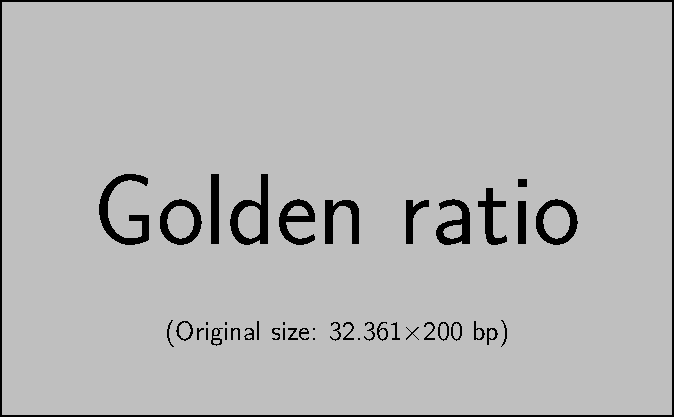
\includegraphics{placeholder_images/example-image-golden.pdf}
    \caption[Charge-transer and basic working mechanism of a Li-ion cell]{Simplified representation of charge-transfer
    process and illustration of basic working mechanism of a Li-ion cell.}
    \label{fig:chargetransferprocess}
\end{figure}

At fully  charged condition,  the majority  of Lithium in  the system  is stored
within  the  negative  electrode  microstructure.  During  discharge,  \ch{Li^0}
atoms  diffuse  out of  deep  interstitial  sites  towards  the surface  of  the
particles  in  the negative  electrode.  At  the surface  (electrode-electrolyte
interface),  a charge-transfer  process takes  place according  to Butler-Volmer
kinetics~\cref{eq:butlervolmer}, leading to the  formation of \ch{Li^+} ions and
electrons.  The electrons  are passed  to the  external circuit  through \ch{Cu}
current collectors  onto which  the conductive matrix  composed of  the negative
electrode material and binders is coated.  The \ch{Li^+} ions travel through the
electrolyte phase,  crossing the  separator membrane  to the  positive electrode
where they  encounter an  electron influx  from the  external circuit.  A charge
transfer  reaction  takes  place  at  the  surface  of  the  positive  electrode
particles, leading to the formation of neutral \ch{Li^0} atoms that diffuse into
the positive electrode microstructure.

During  the   charging  process,  the   reverse  phenomena  occur.   Lithium  is
de-intercalated  from  the  positive  electrode and  a  similar  charge-transfer
happens  at the  surface,  leading  to the  formation  of  \ch{Li^+} ions  which
reach  the  negative  electrode  by   passing  through  the  separator.  At  the
surface  of  the  negative  electrode particles,  these  ions  absorb  electrons
from  the  external circuit,  leading  to  the  formation of  neutral  \ch{Li^0}
that   diffuses  into   interior   vacant  spaces   in   the  layered   graphite
electrode. The  charge-transfer mechanism  and sequence  of events  are depicted
in~\cref{fig:chargetransferprocess}.
\Cref{eq:NegElectrodeRxn,eq:PosElectrodeRxn} summarise the reactions during the
charging and discharging process at the surfaces of both electrode materials.
\begin{align}
    \ch{Li_{$x$} C                            &<=>[\tiny{discharge}][\tiny{charge}] C + $x$ Li^+ + $x$ e^-}\label{eq:NegElectrodeRxn}\\
    \ch{Li_{1-$x$} M O2 + $x$ Li^+  + $x$ e^- &<=>[\tiny{discharge}][\tiny{charge}] LiMO2}\label{eq:PosElectrodeRxn}
\end{align}
where    \ch{M}   represents    a    transition   metal    compound   such    as
\ch{Ni_{1/3}Co_{1/3}Mn_{1/3}}   (NMC),   \ch{Ni_{0.8}Co_{0.15}Al_{0.05}}   (NCA)
amongst other  choices~\cite{Reddy2011}. Assuming  no loss of  cycleable Lithium
due to  parasitic side  reactions or  through other  mechanisms, the  process is
fully reversible.


The electrochemical potential at each electrode  is dependent upon the extent of
its  lithiation. An  empirical  relationship of  each  electrode's potential  as
a  function  of  its  stoichiometry  can be  obtained,  and  is  dependent  upon
the  specific design  and  material  properties of  each  active material  under
consideration. Finally, the \gls{ocv} of the cell is obtained by subtracting the
negative electrode potential from its positive electrode counterpart.


\section{Battery Modelling}

Through accurate model representations  of the electrochemical-thermal behaviour
of  the cell,  advanced monitoring  and control  strategies can  be deployed  to
tackle  the current  research  topics  in Li-ion  batteries  such as  increasing
cycle-life, improving operational  safety and performance~\cite{Plett2015}. Over
the past  two decades, efforts  have been made  to construct accurate  models to
describe  the physical,  electrical, thermal,  electrochemical and  system-level
performance  of  Li-ion  cells,  leading  to  modelling  strategies  of  various
level  of  sophistication.  For  the  interested  reader,  large  in-roads  into
understanding  the breadth  and  depth  of modelling  of  lithium ion  batteries
can  be  made   from  perusing  comprehensive  books  on  this   topic  such  as
those  by Plett~\cite{Plett2015},  Hariharan~\cite{Hariharan2017}, and  Rahn and
Wang~\cite{Rahn2013}.

The  need  to  address  the  operational challenges  of  lithium  ion  batteries
in   an   embedded   environment   such  as   on-board   an   electric   vehicle
has   led   to  an   increased   impetus   on   the  development   of   advanced
\glspl{bms}~\cite{Bergveld2002}. In vehicular  applications, the only measurable
quantities  of  a  lithium  ion  cell are  its  terminal  voltage,  current  and
temperature. This implies  that several internal states of the  cell such as its
\gls{soc}, whose  real-time computation is  vital to the optimal  performance of
the cell, need to be estimated from these available measurements. Therefore, the
performance  of  a \gls{bms}  for  tasks  such  as  online state  estimation  is
dependent upon  the fidelity  of the underlying  cell model  used. Sophisticated
models of the  cell enable these quantities to be  estimated more accurately and
facilitate the implementation  of advanced control algorithms.  Therefore, it is
imperative  that  the cell  model  used  is suitable  for  being  embedded in  a
real-time \gls{bms}.

Most battery  models have the primary  goal of accurately predicting  the cell's
terminal  voltage  at each  time-step.  This  is so  that  the  output from  the
predictor routine  can be compared  to the  measured voltage and  the difference
between them  may be used in  a suitable corrector-subroutine to  improve future
prediction.  The combined  information from  the model  and measurement  is then
blended in a suitable way to estimate the cell's \gls{soc}.

More   advanced  models   strive   to  provide   insight   into  various   other
physico-chemical quantities  that could  affect the health  of the  battery. The
field of  Li-ion battery modelling can  be classified into two  broad categories
---
\begin{enumerate*}[label=\roman*)]
    \item empirical/ad-hoc \glspl{ecm}, and
    \item detailed  \glspl{pbm} that are based  upon first principles.
\end{enumerate*}
However, these  two approaches are typically  at loggerheads with each  other in
the aspect of their computational complexity.

\subsection{\glsfmtlong{ecm}s}

\glspl{ecm}  employ circuit  elements  such as  voltage  sources, resistors  and
capacitors to  model the behaviour  of batteries at their  electrical terminals.
The cell's  thermal subsystem may  also be  modelled by an  analogous electrical
circuit. The  parameters of the  circuit are  typically functions of  the cell's
current, \gls{soc} and  temperature and can be implemented as  a lookup table by
curve-fitting  the model  to experimental  data. Using  such equivalent  circuit
models, two simple methods are available to compute the cell's \gls{soc} ---
\begin{enumerate*}[label=\itshape\alph*\upshape)]
    \item manufacturer-supplied  lookup table or graph of \gls{ocv} versus \gls{soc}, and
    \item numerically integrating the charge passed in and out of the cell over time, commonly referred to as coulomb counting.
\end{enumerate*}
Both methods are computationally  amenable for small-scale embedded applications
like  consumer  electronics;  however,  neither  one is  robust  to  handle  the
stringent demands in performance imposed  by modern vehicular applications.

Advanced state estimation algorithms such  as nonlinear Kalman filters may still
be able to use \glspl{ecm} as the plant model and obtain reasonable estimates of
the  cell's  \gls{soc}~\cite{Plett2006,  Sun2011}. However,  the  usefulness  of
\glspl{ecm} is limited by the fact that their parameters are derived essentially
by a  curve-fitting process using a  standard set of training  data. Since these
models are  not based on  any physical phenomena,  their ability to  predict the
cell's general behaviour  is extremely poor especially when  subjects to current
profiles well  outside their training  realm. Another important  disadvantage of
equivalent circuit  models is that they  do not allow insights  into the various
internal states of the cell.

\glspl{ecm}  of  lithium  ion  batteries   have  been  extensively  studied  and
are  widely  applied.  However,  the aforementioned  difficulties  render  their
reliability and  accuracy questionable,  especially under highly  demanding load
profiles  experienced by  the battery  packs in  \glspl{xeV}. The  boundaries of
their  performance have  been well-quantified  (see~\cite{Plett2015,Plett2016}).
Although  various estimation  and control  algorithms continue  to be  developed
around them, the  \glspl{ecm} themselves are no longer the  subject of extensive
research. Hence, this thesis does not discuss them further.

\subsection{\glsfmtlong{pbm}s}

\glsreset{pbm}

\glspl{pbm} consist of  governing equations that construct a  realization of the
behaviour of the cell based  upon electrochemical principles such as equilibrium
thermodynamics,  material  diffusion  and  reaction  kinetics.  The  fundamental
advantage  to this  modelling approach  is that  it is  possible to  compute the
evolution of  internal states of  the cell  for arbitrary current  profiles. The
difficulty with  the physics-based  modelling approach  lies with  obtaining the
values  of all  the physical,  geometric, electrochemical,  thermal and  kinetic
parameters  of the  cell. Usually,  these parameters  are closely  guarded trade
secrets by cell cell manufacturers.

In  some  cases, it  may  be  possible to  obtain  a  subset of  these  physical
parameters  can be  obtained  by dissection  of cells  in  an inert  environment
followed  by further  characterisation  through specialised  lab equipment.  For
instance, Ecker~\etal~\cite{Ecker2015} demonstrate  the reverse-engineering of a
\SI{7.5}{\amphour} pouch cell by Kokam  Ltd.\ to obtain its physical parameters.
Nevertheless, this is a tedious process and is feasible only with access to such
specialised lab  equipment. Furthermore, the  results from these  experiments is
susceptible to characterisation errors as well as cell-to-cell variations due to
production spread. Therefore, some form of system identification method needs to
be employed  for estimating the rest  of the physical parameters  required for a
\gls{pbm}.  Furthermore, it  is  a common  practice to  rely  on published  data
for  the values  of  certain cell  parameters  that do  not  depend on  physical
construction, especially for those that remain universally true for a particular
li-ion chemistry.

The challenges involved  in model parametrisation is a research  exercise of its
own merit and  is not addressed in  this thesis. A redeeming factor  is that the
task of  parametrisation is a  one-off problem that  appears early in  the model
deployment  stage,  after which  the  rewards  of  superior performance  of  the
\glspl{pbm} can be reaped. Once  the model parameters are available, \glspl{pbm}
can be used in  aiding a deeper understanding of the working of  the cell and in
answering research  questions that could  otherwise not be answered  with simple
\glspl{ecm}. One area  of focus of this  thesis is to broach  a less-probed area
--- exploring  the possibility  of using  a \gls{pbm}  for the  \emph{design} of
pouch cells used in automotive applications. The author's findings on this topic
shall be presented in~\cref{ch:modelbaseddesign}.

A major disadvantage of \glspl{pbm} from an implementation point of view is that
solving for  the model's field  variables is time-consuming. In  particular, the
more  sophisticated  \glspl{pbm}  require  the use  of  multi-physics  \gls{pde}
solvers  and  hence  are  not  typically  suitable  for  embedded  applications.
Nevertheless,  for   high  performance   applications  such  as   in  automotive
\glspl{bms}  wherein   state-of-health  monitoring  is  crucial,   there  is  an
overwhelming  demand for  obtaining insight  into internal  cell variables.  For
instance, the real-time computation of surface concentration of \ch{Li^0} in the
solid particles enable  the \gls{bms} to avoid regulate power  flow into and out
of the cell to proactively avoid plating and degradation of the cell.

In view of this consideration, model  order reduction techniques are seen as key
enablers that facilitate in porting the  predictive powers of \glspl{pbm} into a
real-time microprocessor. This thesis shall therefore have a strong focus on



Doyle,  Fuller,  and  Newman~\cite{Doyle1993}  developed  an  isothermal  porous
electrode model of the cell capable of describing its internal variables such as
\begin{enumerate*}[label=\itshape\alph*\upshape)]
    \item potential on the solid particles,
    \item potential in the electrolyte solution,
    \item concentration of \ch{Li^0} in the solid particles,
    \item ionic concentration in the electrolyte solution, and
    \item molar flux density of lithium at the solid-electrolyte boundary.
\end{enumerate*}
The most popular computational implementation  of the \gls{dfn} equations is the
\gls{p2d} model.  In the  \gls{p2d} implementation, all  field variables  of the
\gls{dfn} model are  computed at each spatial location location  along the axial
thickness of the cell. The solid  concentration is computed within each particle
in a radial co-ordinate system that is  normal to the axial direction. The axial
and radial dimensions  are coupled at each particle's surface  through the molar
flux density describing the rate of  pore-wall flux that crosses from solid into
electrolyte or vice-versa. The \gls{p2d} implementation of the equations of the
\gls{dfn} model is shown in~\cref{tbl:dfneqns}.

Ragone plot

Different type of cells - Prismatic,  pouch and cylindrical. How pouch cells are
used in automotive industry acknowledge Tesla, but cite counter citations. Layer
photos etc

This  thesis  strives to  represent  all  physical  quantities in  the  standard
International  System  of Units  (SI-Units).  However,  there are  some  notable
exceptions \eg{} for the capacity of a  Li-ion cell, which is represented in the
practical units  of Ampere  hours (\SI{}Ah),  rather than the  base SI  Units of
Coulombs (\SI{}{\coulomb}).  Such exceptions  are made  taking into  account the
prevalent conventions in standard literature.

\fxnote{make a note in the introduction  chapter that the terms cell and battery
    are  used  interchangeably deviating  from  their  precise meaning,  \eg{}  cell
modelling and battery modelling}

% \cite{Grazioli2016a} goes crazy in reviewing the models out there.

% \cite{Seaman2014} provide a comprehensive survey  of the wide range of battery
% models out there.

Based on an isothermal description
Mention  that stuff  is  applicable for  both Lithium  ion  and Lithium  polymer
chemistries.


% -*- root: ../main.tex -*-
%!TEX root = ../main.tex
% this file is called up by main.tex
% content in this file will be fed into the main document
% vim:nospell textwidth=180 foldlevelstart=3 foldlevel=3

% \begin{table}[!htbp]
    \begin{table}[p]
        \centering
        \caption[]{}
        % \label{tbl:charSimspmp2d}
        \begin{threeparttable}
            \begingroup
            \makeatletter\def\f@size{10.0625}\check@mathfonts
            % \addtolength{\jot}{0.75em}
            \addtolength{\jot}{0.875em}
            \begin{tabular*}{\textwidth}{@{} l c r l r @{}}
                \toprule
                Region & Governing equations & \multicolumn{3}{c}{Boundary conditions} \\
                \midrule
                \multicolumn{1}{l |}{\rotatebox[origin=c]{+90}{\makecell{\small Electrodes \\ \small \linnegpos}}} &
                $\begin{aligned} % placement: default is "center", options are "top" and "bottom"
                    \vphantom{\diffp{c_\slsub}{r}{\mathrlap{r = R_\pl}}}
                    \diffp{c_\slsub}{t} &= \frac{D_\slsub}{r^2}\diffp{}{r}\left(r^2 \diffp{c_\slsub}{r} \right) \\
                    \vphantom{\diffp{c_\text{e}}{x}{\mathrlap{x = l_\text{tot}}}}
                    \varepsilon_l \diffp{c_\text{e}}{t} &= \diffp{}{x}\left(D_\effl
                    \diffp{c_\text{e}}{x} \right) + (1 - t^0_\text{+}) a_\slsub j_l \\
                    \vphantom{\diffp{\phi_\text{e}}{x}{\mathrlap{x = 0}}} 0 &= \diffp{}{x}\left(\kappa_\effl \diffp{\phi_\text{e}}{x}\right) + \diffp{}{x}\left(\kappa_\effl \frac{2 R T(t)}{F} (t^0_{+}-1)\diffp{ \ln c_\text{e}}{x}\right) \\
                    \vphantom{\sigma_\effl\!\diffp{\phi_\slsub}{x}{\mathrlap{\substack{\vphantom{\displaystyle M}x = x_\text{pos/sep}\\x = x_\text{neg/sep}}}}} a_\slsub F j_l &= \diffp{}{x}\left(\sigma_\effl \diffp{\phi_\slsub}{x}\right) \\
                    % j_l &= k_\lr c^\alpha_\text{e}\left(c_\slmax - c_\slsurf\right)^\alpha c^\alpha_\slsurf\left( \exp\left(\frac{\left(1-\alpha\right)F}{R T}\eta\right) - \exp\left(-\frac{\alpha F}{R T}\eta\right) \right)
                    j_l &= 2 k_\lr \sqrt{c_\text{e}\left(c_\slmax - c_\slsurf\right) c_\slsurf} \sinh \left(\frac{0.5 F}{R T(t)} \eta_l \right)
                \end{aligned}$ &
                $\begin{aligned}
                    \vphantom{\diffp{c_\slsub}{r}{\mathrlap{r = R_\pl}}} \diffp{c_\slsub}{r}{\mathrlap{r = 0}}\hspace{1mm} &= 0, \\
                    \vphantom{\diffp{c_\text{e}}{x}{\mathrlap{x = l_\text{tot}}}} \diffp{c_\text{e}}{x}{\mathrlap{x = 0}}\hspace{1mm} &= 0, \\
                    \diffp{\phi_\text{e}}{x}{\mathrlap{x = 0}}\hspace{1mm} &= 0, \\
                    \sigma_\effl\!\diffp{\phi_\slsub}{x}{\mathrlap{\substack{\vphantom{\displaystyle M}x = x_\text{pos/sep}\\x = x_\text{neg/sep}}}}\hspace{1mm} &= 0, \\
                    % {}&\textemdash{}{}
                    {}&\xdash[1.25em]{}
                \end{aligned}$ &
                $\begin{aligned}
                    \diffp{c_\slsub}{r}{\mathrlap{r = R_\pl}}\hspace{1mm} &= \frac{-j_l}{D_\slsub} \\
                    \diffp{c_\text{e}}{x}{\mathrlap{x = l_\text{tot}}}\hspace{1mm} &= 0 \\
                \vphantom{\diffp{\phi_\text{e}}{x}{\mathrlap{x = 0}}} \phi_\text{e}\Bigr\rvert_{\mathrlap{x=l_\text{tot}}} \hspace{1mm}&= 0 \\
                % \sigma_\effl\!\diffp{\phi_\slsub}{x}{\mathrlap{\subalign{x&=0\\x&=x_\text{tot}}}} &= \frac{-I}{A} \\
                \vphantom{\sigma_\effl\!\diffp{\phi_\slsub}{x}{\mathrlap{\substack{\vphantom{\displaystyle M}x = x_\text{pos/sep}\\x = x_\text{neg/sep}}}}} \sigma_\effl\!\diffp{\phi_\slsub}{x}{\mathrlap{\substack{\!\!\!\!\!x=0\\x=x_\text{tot}}}}\hspace{1mm} &= \frac{-I}{A} \\
                % \sigma_\effl\!\diffp{\phi_\slsub}{x}{\mathrlap{\substack{\begin{mysubarray} x &=0 \\ x &=x_\text{tot}\end{mysubarray}}}} &= \frac{-I}{A} \\
                % {}&\textemdash{}{}
                {}&\xdash[1.25em]{}
            \end{aligned}$ &
            $\begin{aligned}
                \vphantom{\diffp{c_\slsub}{r}{\mathrlap{r = R_\pl}}}\refstepcounter{equation}(\theequation)\label{eq:dfnsoliddiff} \\
                \vphantom{\diffp{c_\text{e}}{x}{\mathrlap{x = l_\text{tot}}}} \refstepcounter{equation}(\theequation)\label{eq:dfnliquiddiff} \\
                \vphantom{\diffp{\phi_\text{e}}{x}{\mathrlap{x = 0}}} \refstepcounter{equation}(\theequation) \\
                \vphantom{\sigma_\effl\!\diffp{\phi_\slsub}{x}{\mathrlap{\substack{\vphantom{\displaystyle M}x = x_\text{pos/sep}\\x = x_\text{neg/sep}}}}} \refstepcounter{equation}(\theequation) \\
                \vphantom{\left(\frac{0.5 F}{R T(t)} \eta \right)} \refstepcounter{equation}(\theequation)
            \end{aligned}$ \\
            \bottomrule
        \end{tabular*}
        \endgroup
        \begin{minipage}{\textwidth}
            \bigskip
            \begin{flushleft}
                \raggedright
                \makeatletter\def\f@size{14}\check@mathfonts
                $\begin{alignedat}{2}
                    & \text{\textbullet{} } c_\text{e} &  & \coloneqq c_\text{e}(x,t), \quad  \{x \in [0,l_\text{tot}],\, (x=0)\symbol{"2259} \text{\footnotesize pos/Alcc},\, (x=l_\text{tot})\symbol{"2259} \text{\footnotesize neg/Cucc}\}  \tnote{\dagger}                                                                                                                                                                  \\
                    & \text{\textbullet{} } \phi_\text{e} &  & \coloneqq \phi_\text{e}(x,t)\\
                \end{alignedat}$
                \\[0.5em]
                \fbox{\raggedright \small  \linnegpos}
                $\begin{alignedat}{2}
                    % & \mathbf{\textbf \linnegpos} & {} \\
                    & \text{\textbullet{} } c_\slsub   &  & \coloneqq c_\slsub(r,t), \quad  \{r \in [0,R_\pl],\, (r=0)\symbol{"2259} \text{\footnotesize  particle center},\, (r=R_\pl)\symbol{"2259} \text{\footnotesize particle surface}\}              \\
                    & \text{\textbullet{} } c_\slsurf &  & \coloneqq c_\slsub(r=R_\pl,t)\\
                    & \text{\textbullet{} } \phi_\slsub &  & \coloneqq \phi_\slsub(x,t)\\
                    & \text{\textbullet{} } j_l          &  & \coloneqq j_l(x,t) \\
                    & \text{\textbullet{} } \sigma_\effl &  & = \sigma_l \cdot \varepsilon_l \\
                    & \text{\textbullet{} } \eta_l        &  & \coloneqq \eta_l(x,t) = \phi_\slsub(x,t) - \phi_\text{e}(x,t) - \mathcal{U}_l(c_\slsurf) \\[0.5em]
                \end{alignedat}$
                % \medskip
                \fbox{\raggedright \small  \linnegseppos}\\[0.5ex]
                $\begin{alignedat}{2}
                    & \text{\textbullet{} } D_\effl    &  & = D \cdot \varepsilon_l^{\text{brugg}_l}                                                                                                                                                  \\
                    & \text{\textbullet{} } \kappa_\effl &  & = \kappa \cdot \varepsilon_l^{\text{brugg}_l} \\
                    & \text{\textbullet{} } D        &  & \coloneqq D(c_\text{e},T) = 10^{-4} \times 10^{-4.43 - \frac{54}{T(t) - 229 - 5\times10^{-3} c_\text{e}(x,t)} - 0.22\times10^{-3} c_\text{e}(x,t)}               \\
                \end{alignedat}$
                \\
                \makeatletter\def\f@size{14}\check@mathfonts
                $\begin{alignedat}{2}
                    & \text{\textbullet{} }  \kappa   \: \quad&  & \coloneqq \kappa(c_\text{e},T)\, = \parbox[t]{11.60cm}{\raggedright $\scriptstyle 10^{-4} \times c_\text{e}(x,t)\Big(-10.5 + 0.668\times10^{-3} c_\text{e}(x,t) + 0.494\times10^{-6} c_\text{e}^2(x,t) + \big(0.074 - 1.78\times10^{-5}c_\text{e}(x,t) - 8.86\times10^{-10}c_\text{e}^2(x,t)\big)T(t) + \big(-6.96\times10^{-5} + 2.8\times10^{-8} c_\text{e}(x,t)\big)T^2(t)\Big)^2$}\\
                \end{alignedat}$
            \end{flushleft}
        \end{minipage}
        \bigskip
        \footnoterule{}
        \begin{tablenotes}
        \item[\dagger] \footnotesize{This definition of the global axial domain $x$, spanning the cell thickness applies for all variables dependent on axial spatial position. Hence the domain definition for $x$ is not repeated elsewhere for the sake of brevity.}
        \end{tablenotes}
    \end{threeparttable}
\end{table}


% write about lumped thermal model equations here. Point out to relevant
% parameters


% \fxnote{Where does  this paragraph go? End  of this section/end of  chapter or
% even  last  chapter?}  The  identification of  individual  parameters  of  the
% \gls{dfn} model  remains a  key area  in battery  modelling that  remains only
% partially  explored. Nevertheless,  this effort  is critical  to ensure  rapid
% adoption  of any  physics-based  model and  sophisticated control  algorithms.
% The  state of  the  art in  this  area, the  challenges  involved and  current
% efforts  in  this  direction are  explored  in~\cref{ch:futurework}.  Although
% sensitivity  analysis  of  the  \gls{dfn} parameters  has  been  performed  in
% literature, \fxnote{citation here} the extent to which parameter uncertainties
% influence  the   numerical  values  in  the   $A,  B,  C$  and   $D$  matrices
% of~\Cref{eq:LTIstatespace} has not yet been attempted. In continuation of this
% research aspect, the order of magnitude  shift in eigen/singular values of the
% relevant system matrix also need to be quantified to enable an informed choice
% about stability of such models for real-time implementations.

 % Introduction (to do later)
% -*- root: ../thesis.tex -*-
%!TEX root = ../thesis.tex
% ******************************* Thesis Chapter 2 ****************************


% ----------------------- paths to graphics ------------------------

% change according to folder and file names
\graphicspath{{2/figures/}}
% ----------------------- contents from here ------------------------

\section{Lorem ipsum}

Lorem ipsum dolor sit amet, consectetur adipiscing elit. Sed vitae laoreet lectus. Donec lacus quam, malesuada ut erat vel, consectetur eleifend tellus. Aliquam non feugiat lacus. Interdum et malesuada fames ac ante ipsum primis in faucibus. Quisque a dolor sit amet dui malesuada malesuada id ac metus. Phasellus posuere egestas mauris, sed porta arcu vulputate ut. Donec arcu erat, ultrices et nisl ut, ultricies facilisis urna. Quisque iaculis, lorem non maximus pretium, dui eros auctor quam, sed sodales libero felis vel orci. Aliquam neque nunc, elementum id accumsan eu, varius eu enim. Aliquam blandit ante et ligula tempor pharetra. Donec molestie porttitor commodo. Integer rutrum turpis ac erat tristique cursus. Sed venenatis urna vel tempus venenatis. Nam eu rhoncus eros, et condimentum elit. Quisque risus turpis, aliquam eget euismod id, gravida in odio. Nunc elementum nibh risus, ut faucibus mauris molestie eu.
 Vivamus quis nunc nec nisl vulputate fringilla. Duis tempus libero ac justo laoreet tincidunt. Fusce sagittis gravida magna, pharetra venenatis mauris semper at. Nullam eleifend felis a elementum sagittis. In vel turpis eu metus euismod tempus eget sit amet tortor. Donec eu rhoncus libero, quis iaculis lectus. Aliquam erat volutpat. Proin id ullamcorper tortor. Fusce vestibulum a enim non volutpat. Nam ut interdum nulla. Proin lacinia felis malesuada arcu aliquet fringilla. Aliquam condimentum, tellus eget maximus porttitor, quam sem luctus massa, eu fermentum arcu diam ac massa. Praesent ut quam id leo molestie rhoncus. Praesent nec odio eget turpis bibendum eleifend non sit amet mi. Curabitur placerat finibus velit, eu ultricies risus imperdiet ut. Suspendisse lorem orci, luctus porta eros a, commodo maximus nisi.

Nunc et dolor diam. Phasellus eu justo vitae diam vehicula tristique. Vestibulum vulputate cursus turpis nec commodo. Etiam elementum sit amet erat et pellentesque. In eu augue sed tortor mollis tincidunt. Mauris eros dui, sagittis vestibulum vestibulum vitae, molestie a velit. Donec non felis ut velit aliquam convallis sit amet sit amet velit. Aliquam vulputate, elit in lacinia lacinia, odio lacus consectetur quam, sit amet facilisis mi justo id magna. Curabitur aliquet pulvinar eros. Cras metus enim, tristique ut magna a, interdum egestas nibh. Aenean lorem odio, varius a sollicitudin non, cursus a odio. Vestibulum ante ipsum primis in faucibus orci luctus et ultrices posuere cubilia Curae; 
\begin{enumerate}
\item one
\item two
\begin{enumerate}
\item two one
\item two two
\end{enumerate}
\item three
\end{enumerate}
Morbi bibendum est aliquam, hendrerit dolor ac, pretium sem. Nunc molestie, dui in euismod finibus, nunc enim viverra enim, eu mattis mi metus id libero. Cras sed accumsan justo, ut volutpat ipsum. Nam faucibus auctor molestie. Morbi sit amet eros a justo pretium aliquet. Maecenas tempor risus sit amet tincidunt tincidunt. Curabitur dapibus gravida gravida. Vivamus porta ullamcorper nisi eu molestie. Ut pretium nisl eu facilisis tempor. Nulla rutrum tincidunt justo, id placerat lacus laoreet et. Sed cursus lobortis vehicula. Donec sed tortor et est cursus pellentesque sit amet sed velit. Proin efficitur posuere felis, porta auctor nunc. Etiam non porta risus. Pellentesque lacinia eros at ante iaculis, sed aliquet ipsum volutpat. Suspendisse potenti.

Ut ultrices lectus sed sagittis varius. Nulla facilisi. Nullam tortor sem, placerat nec condimentum eu, tristique eget ex. Nullam pretium tellus ut nibh accumsan elementum. Aliquam posuere gravida tellus, id imperdiet nulla rutrum imperdiet. Nulla pretium ullamcorper quam, non iaculis orci consectetur eget. Curabitur non laoreet nisl. Maecenas lacinia, lorem vel tincidunt cursus, odio lorem aliquet est, gravida auctor arcu urna id enim. Morbi accumsan bibendum ipsum, ut maximus dui placerat vitae. Nullam pretium ac tortor nec venenatis. Nunc non aliquet neque. 

\section{Some math}
\begin{theorem}[Residue Theorem]
Let $f$ be analytic in the region $G$ except for the isolated 
singularities $a_1,a_2,\dots,a_m$. If $\gamma$ is a closed 
rectifiable curve in $G$ which does not pass through any of the 
points $a_k$ and if $\gamma\approx 0$ in $G$, then
\[
  \frac{1}{2\pi i}\int_\gamma\! f = \sum_{k=1}^m 
  n(\gamma;a_k)\textnormal{Res}(f;a_k)\,.
\]
\end{theorem}
\subsection{More math}
$y =
\sin(x)$:
\begin{equation}
  y = \int_0^x\cos(x)\,\mathrm{d}{x} = \frac{e^{\mathrm{i} x} - e^{-\mathrm{i} x}}{2\mathrm{i}}
\end{equation}
Normal text output.
 \textsf{This is written with textsf!}
 \textbf{And this text with textbf!}
 \texttt{This is Courier font.}


\section{Preliminary aims}

Morbi bibendum est aliquam, hendrerit dolor ac, pretium sem. Nunc molestie, dui in euismod finibus, nunc enim viverra enim, eu mattis mi metus id libero. Cras sed accumsan justo, ut volutpat ipsum. Nam faucibus auctor molestie. Morbi sit amet eros a justo pretium aliquet. Maecenas tempor risus sit amet tincidunt tincidunt. Curabitur dapibus gravida gravida. Vivamus porta ullamcorper nisi eu molestie. Ut pretium nisl eu facilisis tempor. Nulla rutrum tincidunt justo, id placerat lacus laoreet et. Sed cursus lobortis vehicula. Donec sed tortor et est cursus pellentesque sit amet sed velit. Proin efficitur posuere felis, porta auctor nunc. Etiam non porta risus. Pellentesque lacinia eros at ante iaculis, sed aliquet ipsum volutpat. Suspendisse potenti.

Ut ultrices lectus sed sagittis varius. Nulla facilisi. Nullam tortor sem, placerat nec condimentum eu, tristique eget ex. Nullam pretium tellus ut nibh accumsan elementum. Aliquam posuere gravida tellus, id imperdiet nulla rutrum imperdiet. Nulla pretium ullamcorper quam, non iaculis orci consectetur eget. Curabitur non laoreet nisl. Maecenas lacinia, lorem vel tincidunt cursus, odio lorem aliquet est, gravida auctor arcu urna id enim. Morbi accumsan bibendum ipsum, ut maximus dui placerat vitae. Nullam pretium ac tortor nec venenatis. Nunc non aliquet neque. 

Morbi bibendum est aliquam, hendrerit dolor ac, pretium sem. Nunc molestie, dui in euismod finibus, nunc enim viverra enim, eu mattis mi metus id libero. Cras sed accumsan justo, ut volutpat ipsum. Nam faucibus auctor molestie. Morbi sit amet eros a justo pretium aliquet. Maecenas tempor risus sit amet tincidunt tincidunt. Curabitur dapibus gravida gravida. Vivamus porta ullamcorper nisi eu molestie. Ut pretium nisl eu facilisis tempor. Nulla rutrum tincidunt justo, id placerat lacus laoreet et. Sed cursus lobortis vehicula. Donec sed tortor et est cursus pellentesque sit amet sed velit. Proin efficitur posuere felis, porta auctor nunc. Etiam non porta risus. Pellentesque lacinia eros at ante iaculis, sed aliquet ipsum volutpat. Suspendisse potenti.

Ut ultrices lectus sed sagittis varius. Nulla facilisi. Nullam tortor sem, placerat nec condimentum eu, tristique eget ex. Nullam pretium tellus ut nibh accumsan elementum. Aliquam posuere gravida tellus, id imperdiet nulla rutrum imperdiet. Nulla pretium ullamcorper quam, non iaculis orci consectetur eget. Curabitur non laoreet nisl. Maecenas lacinia, lorem vel tincidunt cursus, odio lorem aliquet est, gravida auctor arcu urna id enim. Morbi accumsan bibendum ipsum, ut maximus dui placerat vitae. Nullam pretium ac tortor nec venenatis. Nunc non aliquet neque. 




% ---------------------------------------------------------------------------
% ----------------------- end of thesis sub-document ------------------------
% --------------------------------------------------------------------------- % Literature Review
% \setcounter{chapter}{2} % Temporary for layer opt chapter plan
% -*- root: ../main.tex -*-
%!TEX root = ../main.tex

\graphicspath{{3/figures/}}
% ----------------------- contents from here ------------------------

\chapter{Model-based Design Of Pouch Cells}\label{ch:modelbaseddesign}
\startcontents[chapters]
\printcontents[chapters]{}{1}{\setcounter{tocdepth}{1}}

\bigskip
Intro here \dots

\section{Hybrid Finite Volume-Spectral Scheme}\label{sec:hybrid fv-spectral}

 % Layer Optimisation
% -*- root: ../main.tex -*-
%!TEX root = ../main.tex
% this file is called up by main.tex
% content in this file will be fed into the main document
% vim:textwidth=80 fo=cqt

%level followed %by section, subsection


% ----------------------- paths to graphics ------------------------

% change according to folder and file names
\graphicspath{{4/figures/}}
% ----------------------- contents from here ------------------------

\todo{uncomment and edit the intro in the source code later on}

% Battery modellers face the classic  conundrum of conjuring physics-based battery
% models that remain  amenable for control applications.  Firstly, the contrasting
% nature of this modelling objective is presented. Secondly, prior attempts by the
% research community to  tackle this issue is briefly examined.  A suitable family
% of models  from the broad  category of reduced-order  models is identified  as a
% promising  candidate  for implementation  in  controls  applications. Next,  the
% drawbacks of this family of models is  discussed in detail. The state of the art
% implementation for tackling these drawbacks  is presented and their inadequacies
% are discussed.


\todo{Write the chapter. Finally come back to summarize this}


% The following efforts/trials were done (failures)
% \begin{itemize}
%     \item first attempt
%     \item second attempt
% \end{itemize}
% The following successes were achieved.
% \begin{itemize}
%     \item first attempt
%     \item second attempt
% \end{itemize}


% At the  end of this  chapter, we have a  control oriented reduced  order battery
% model amenable for use in real-time applications for SOC, SOH etc.\ estimations.


Control-Oriented  models can  be considered  synonymous with  the term  `Reduced
Order Models'. This is because the complexity of physics-based models inherently
necessitates the  use of a low  order model. In  this thesis, the two  terms are
used interchangeably.


\section{Reduced Order Models: A New Classification Scheme}\label{sec:classificationscheme}

Jokar~\etal~\cite{Jokar2016}  provide  a  comprehensive review  of  the  various
categories  of  reduced  order  physics  based  battery  models.  However,  this
work  does  not aim  to  classify  models  based on  time-vs-frequency  domains.
Fan~\etal{}~\cite{Fan2015}  conducted  a  review   of  reduced  order  modelling
methods, but  only provide an  overview of  deriving and implementing  models in
these  dual domains  without expository  analysis  of the  implications of  this
modelling choice. Unlike~\cite{Jokar2016}, this review  did not aim to provide a
classification  of various  reduced order  models, but  instead emphasises  on a
broad survey of relevant methodologies  and tools towards obtaining such models.
Hence,  neither~\cite{Jokar2016}  nor~\cite{Fan2015}  provide insight  into  the
rubrics and  implications of  the choice  of modelling in  either of  these dual
domains. Although in principle, the transformation between them follows standard
mathematical  practices,\todo{citation(s)  needed?}availability  of  models  for
final implementation  in the time domain  aids immediate uptake by  industry for
adoption  in online  \gls{bms}s. Treatment  of  reduced order  models from  this
aspect  is so  germane to  the central  hypothesis of  this chapter,\todo{can  a
simple time  domain model  do the  job?} that  the author  of this  thesis feels
compelled to undertake  a simpler classification exercise within  the context of
suitability for online implementation.


In this discussion,  various modelling methodologies and  their resultant models
are viewed  as a single  continuum and  consequently this thesis  discusses them
from such a unified perspective. Furthermore,  there is also a need to highlight
the  salient  works among  the  more  recent  advances  and extensions  to  then
prevailing  models published  since~\cite{Jokar2016} and~\cite{Fan2015}.  Hence,
the specialised  review of  reduced order modelling  literature covered  in this
section intends to supplement --- not  supplant --- the breadth of modelling art
covered between them. In particular, care  has been taken to minimize repetition
of  background art  already analysed  in these  aforementioned review  articles,
thereby striving  to report the  subset of prior  research that is  pertinent to
illustrate the  new classification scheme  introduced here. The author  does not
aim to adhere  to a chronological presentation of such  background art. Instead,
the salient  model families are  introduced in  the context of  discussing their
significance within a particular modelling technique.



Physics-based control-oriented models  can be classified as belonging  to one of
the following categories.\todo{just enumerate my classification in-line here} It
is important to distinguish between models that are derived directly in the time
domain versus  those that are  derived first in  the frequency domain  and later
converted to time domain.
\todo{enumerate all the desirable characteristics and criterion upon which
models are to be evaluated}


In  principle,  any modelling  method  that  yields a  time domain  mathematical
description of physical  phenomena that is lower in  computational complexity by
an arbitrary magnitude  than the original \gls{dfn} model can  be considered for
further investigation. In the absence of a canonical, quantitative definition of
what  constitutes a  reduced  order model,  the number  of  candidate family  of
models  to  consider  is  overwhelmingly large\todo{is  it  appropriate  to  use
such  language?}.  In  practice,  the  constraints  and  challenges  imposed  by
the  scope  of  this  work, \viz{}  suitability  for  real-time  implementation,
limits  the  choice  of  candidate  modelling  families.  For  instance,  models
relying  primarily on  classical finite  difference~\cite{Smith2006}, Galerkin's
approximation~\cite{Dao2012} or Galerkin's projection~\cite{Fan2018} methods for
transformation  and order  reduction  of  one or  more  field  variables of  the
\gls{dfn} model  are excluded. This is  done in view of  the impracticability of
implementing  such  models in  a  resource-constrained  environment such  as  an
embedded \gls{bms} controller.


Owing to  the low entry-barrier for  adoption in a real-time  controller logging
data samples  at specific time intervals,  this chapter focusses on  models that
are cast  in a  form for final  implementation in the  time domain.  This choice
implies the exclusion of those models  that are derived and implemented entirely
in the frequency domain. For the  sake of readers interested in frequency domain
methods, the discussion here briefly introduces salient literature employing the
Padé  approximation method  that serves  as  a backbone  of a  wide variety  of
frequency domain models.


\todo{can  mention  that  most  frequency domain  models  are  impedance  models
suitable for offline simulation eg An electrochemistry-based impedance model for
lithium-ion batteries}


The     transfer     function     oriented    Padé     approximation     method
for    low    order    physics-based     battery    modelling    pioneered    by
Forman~\etal{}~\cite{Forman2011a}    has   gained    widespread   adoption    in
the    areas     of    cell     design~\cite{Marcicki2013},    charge-trajectory
optimisation~\cite{Bashash2010},    controller    design~\cite{Perez2015}    and
state    estimation~\cite{Marcicki2013,Moura2012}.     Although    Prasad    and
Rahn~\cite{Prasad2013} present  an online identification  of a subset  of ageing
parameters using a Padé model and a recursive least squares algorithm, specific
implementation details such as the transformation of the Padé reduced impedance
to  discrete-time  difference  equations  was not  provided.  Padé  models  are
typically limited  to offline  applications owing  to the  aggressive trade-offs
required in the approximation order to maintain accuracy. Those models truncated
to  very low  Padé  order exhibit  poor  fidelity and  perform  no better  than
classical  equivalent circuit  models,  although recent  research attempts  have
focussed  to  mitigate  this  drawback~\cite{Yuan2017a,Yuan2017}.\todo{Should  I
discuss how they mitigated this?}


Smith~\etal{}~\cite{Smith2007}  pioneered   a  semi-hybrid   modelling  approach
to  reduced  order  modelling  and  obtained closed  form  expressions  for  all
electrochemical field variables  in the frequency domain  except for electrolyte
concentration and  potential (which were  solved separately using  the classical
finite difference discretization method). To the author's knowledge, this is the
earliest  published  instance  wherein  all  the  dynamics  of  the  full  order
model were  completely retained  in the frequency  domain. This  was facilitated
through  the use  of  transcendental  transfer functions  that  helped to  avoid
the  accuracy  degradation  brought  about  by  truncation  techniques  such  as
Padé  approximation. A  composite impedance  model was  obtained that  was then
converted  to  a  \engordnumber{12}  order state  space  model  through  residue
grouping  and truncation  techniques.  To  the knowledge  of  this author,  this
represents the first  instance in published literature  demonstrating a complete
hybrid  modelling workflow.  This model  was  capable of  predicting the  cell's
terminal voltage  within \SI{1}{\percent} of  a full-order \gls{dfn}  model. The
lumped impedance  model was  derived for  the frequency  range of  interest from
\SIrange{0}{10}{\hertz}.

This modelling effort  by Smith~\etal{} was the  first of its kind  to provide a
physics-based  battery model  for  implementation in  the classical  state-space
formulation
\begin{equation}\label{eq:statespace}
    \begin{aligned}
        \dot{x} &= Ax + Bu \\
        y &= Cx + Du
    \end{aligned}
\end{equation}
that is amenable for controller  design and  further system-level simulation
studies \eg{}  as a component in a (hybrid) electric vehicle drivetrain.


The requirement of a relatively large number of state variables (12) to describe
the system dynamics dilutes the effectiveness of state estimation algorithms. In
the classical isothermal implementation of  this model, with the cell's terminal
voltage being the only measured quantity, the observablity of the model degrades
significantly. Although Smith~\etal{} performed  an observablity analysis of the
model in  a noise-free context,  the presence  of process noise  (via unmodelled
electrochemical phenomena  and parameter uncertainties) coupled  with corruption
of measurement  values through  sensor noise in  a harsh  electrical environment
such as  in an  vehicle's drivetrain,  makes this  model unattractive  for state
estimation tasks in an online embedded application.


Several attempts have been undertaken to  improve and extend the ideas pioneered
in  Smith~\etal{}~\cite{Smith2007}.  Lee~\etal{}~addressed  a  critical  missing
aspect  of~\cite{Smith2007}, \viz{}  the derivation  of transcendental  transfer
functions  for  both the  electrolyte  concentration  and its  potential.  These
transfer  functions  were  obtained  by  using  a  Sturm-Liouville  approach  by
retaining  the first  five modes  of  the eigenfunction  expansion, as  detailed
in~\cite{Lee2012}. To the  author's best knowledge, this is  the first published
work wherein  all electrochemical  field variables of  the \gls{dfn}  model were
considered  for inclusion  in a  deterministic model  order reduction  procedure
whilst retaining the derivation entirely in the frequency domain.


Obtaining  closed form  expressions for  the electrolyte  variables achieved  in
Lee~\etal{} also has an important computational implication. With these capstone
derivations serving to completing the model description in the frequency domain,
all  electrochemical  variables of  the  \gls{dfn}  model  could now  be  solved
independently at any  desired spatial location, \eg{} at  the current collectors
and separator  interfaces. Until  this point,  the state of  the art  in reduced
order  modelling invariably  necessitated  the solution  of all  electrochemical
quantities at  multiple node locations along  the thickness of each  cell layer,
adding  to the  computational burden.  This is  a significant  deterrent to  the
adoption  of such  models if  the intended  purpose of  the model  is to  simply
predict the cell's terminal voltage.


Furthermore,  Lee~\etal{}~\cite{Lee2012a} also  devised the  \gls{dra}, a  novel
algorithm  to systematically  transform  all  transcendental transfer  functions
to  the  time domain   to  obtain  the  standard  state-space   model  given  by
\cref{eq:statespace}. The  author of  this thesis  considers the  formulation of
the  \gls{dra}  as a  breakthrough  contribution  that  has helped  in  bringing
physics-informed  time domain  models a  step  closer  to online  implementation
without   having  to   resort   to   forming  a   lumped   impedance  and   then
truncating  it  suitably.  Lee~\etal{}~\cite{Lee2014} then  extended  this  work
for  a  wider range  of  operation  across  various \gls{soc},  temperature  and
C-rates.  Although the  final  state space  model is  simple  to implement,  the
classical  \gls{dra} scheme  proposed  by Lee~\etal{}  suffers from  significant
computational bottlenecks  in forming the required  block-Hankel matrices during
the  model-derivation  phase.  A   memory-efficient  version  of  the  \gls{dra}
exploiting the  skew-symmetric structure of  these Hankel matrices  was proposed
in  Gopalakrishnan~\etal{}~\cite{Gopalakrishnan2017}  resulting  in  drastically
reduced requirements for physical memory and processing power.


In both the original  as well as the improved \gls{dra},  the computation of the
eigenfunction modal expansion of electrolyte concentration transfer function was
computationally intensive.  A less  severe disadvantage with  the transcendental
transfer  functions  associated  with  the electrolyte  concentration  was  that
their  derivation  entailed  mathematically  cumbersome  symbolic  manipulations
that  dictated  the   need  of  a  capable  \gls{cas}   package.  Although  from
a  stand-alone  viewpoint  this  requirement  does  not  seem  to  be  critical,
the  Ho-Kalman  algorithm   that  forms  a  core  component   of  the  \gls{dra}
schemes  is  steeped in  numerical  linear  algebra routines.  Furthermore,  for
facilitating  state  estimator  and  controller designs,  it  is  convenient  to
implement the resultant  state-space model in a  classical numerical computation
environment   such  as   \textsc{MATLAB}.  Taking   these  into   consideration,
Rodriguez~\etal{}~\cite{Rodriguez2017}  introduced a  simplified computation  of
the electrolyte  concentration transfer  function by  applying the  variation of
parameters  (VOP)  scheme.  With  this  final  improvement,  the  hybrid  scheme
envisaged originally by Lee~\etal{} can  be considered feature-complete with low
computational  requirements  during  both model  derivation  and  implementation
phase.


A  key  drawback  of  the  transcendental  transfer  function  approach  is  the
requirement for  linearisation at  a specific \gls{soc}.  This implies  that the
entries in  the matrices of the  state space model depends  on the linearisation
point.  In all  the  published  works employing  this  approach, these  transfer
functions were obtained  by linearising the \gls{p2d} equations  at an operating
point of  \SI{50}{\percent} \gls{soc}. The requirement  of linearisation renders
the  model usable  only  in  a narrow  range  of  \gls{soc}s. Furthermore,  this
adversely affects the usability of the model for state estimation tasks, wherein
the \gls{soc} is in fact an unknown quantity and is to be estimated.


In order  to extend  the model's  range of  validity, Lee~\etal{}~\cite{Lee2014}
proposed  a  simple model-blending  approach  by  interpolating between  several
linear models pre-computed at  different \gls{soc} and temperature combinations.
To guarantee robustness during cross-over, a  naive approach is to incorporate a
large  number  of  break-points  in  the  look-up  table.  Since  the  model  is
intended  for  online  operation,  this would  entail  significant  requirements
of  both operating  memory  and non-volatile  storage.  An alternative  approach
is  to  implement  a  fairly  coarse  break-point  table  with  a  sophisticated
changeover  mechanism. However,  this  demands careful  tuning  of the  blending
parameters  and  gain values,  an  in-depth  treatment  of  which has  not  been
detailed in Lee~\etal~\cite{Lee2014}.  Furthermore, employing these interpolated
matrices---whose  entries are  obtained  from pre-computed  matrices at  various
\gls{soc}s and temperature---for state-estimation  creates a subtle cyclic loop.
The stability  of this feedback loop  hence introduced has not  been analysed in
literature.  This  renders the  idea  of  state-estimation using  such  run-time
interpolated models  questionable.


The author  of this thesis hypothesises  that any perceivable drawbacks  such as
non-smooth changes  in \gls{soc} estimates  arising from using  blended matrices
could  be potentially  mitigated by  using  smoothing filters  and other  ad-hoc
apparatus.  However,  there  exists  no  published  work  that  discusses  these
engineering aspects. Coupled with the absence  of a theoretical analysis of loop
stability,  these  models  are  deemed  as  not  being  suitable  for  immediate
adoption  by  industry, at  least  until  these  aforementioned gaps  have  been
addressed  satisfactorily.  The non-linear  state  variable  model presented  by
Guo~\etal{}~\cite{Guo2017} aims to  address this issue by  formulating a reduced
order model in  the frequency domain by eliminating  linearisation. However, the
online solution of the model entails an complex prediction-refinement procedure,
loosely defined as implicit and explicit solution methods, for each subsystem of
the  \gls{dfn}  model.  The  formulation  of the  final  model  is  not  clearly
illustrated and  in the views of  this author, is not  easily comprehensible. In
the absence  of actual source  code, a numerical  example or pseudo-code  of the
model reduction workflow could have immensely helped with the reproducibility of
the results claimed in the work.


Physics-inspired                        equivalent                       circuit
models~\cite{Prasad2012,Prasad2014,Zhang2017,Cheng2017,Merla2018} are a class of
hybrid  models  that  have  rapidly  gained  prominence  since  the  publication
of~\cite{Jokar2016}  and~\cite{Fan2015}. The  derivation of  the relevant  model
equations  is  performed   in  the  frequency  domain.   This  frequency  domain
representation is  then converted to  a form  suitable for implementation  as an
equivalent circuit. Prasad and Rahn~\cite{Prasad2014} extended their Padé order
reduced  model first  presented  in~\cite{Prasad2013} to  convert the  impedance
model into standard  equivalent circuits. A key point to  be highlighted is that
these family of models do not necessarily strive to retain the classical Randles
structure~\cite{Randles1947}  for   their  equivalent   circuit  representation.
Instead,  the  values  of  the  electrical circuit  components  such  as  series
resistance and  equivalent capacitance  are obtained through  various mechanisms
such as \gls{eis} measurements under load.  The biggest advantage of such models
is that  they serve  as drop-in replacements  to traditional  equivalent circuit
models whilst still  retaining their origins in physical  principles rather than
on empirical curve-fitting.


\todo{can perhaps  talk about SPM converted  to equivalent circuit by  Prasad in
the IEEE conference paper}


\Cref{ch:chapter6}  briefly presents  the author's  latest work  and preliminary
results towards  obtaining a similar physics-informed  equivalent circuit model.
This  modelling  effort is  a  direct  application  of  the gains  in  computing
efficiency  through  the  application  of the  improved  \gls{dra}  reported  in
Gopalakrishnan~\etal{}~\cite{Gopalakrishnan2017},   the  detailed   coverage  of
which  is performed  in~\cref{ch:chapter3}.  This work  intends  to address  the
hitherto  unexplored  gap  in  impedance  modelling, \ie{}  the  absence  of  an
equivalent impedance  model that  accounts for  the impedance  contribution from
all  electrochemical quantities  in the  \gls{p2d} model.  This physics-informed
impedance  model can  be  extended  to fit  parameter  values  of components  in
an  equivalent circuit  model,  \eg{} by  using  a standard  Levenberg-Marquardt
non-linear least squares fitting algorithm~\cite{Levenberg1944, Marquardt1963}.


A common characteristic of  all hybrid models is the lack  of a physical meaning
to their  model parameters. This  severely limits  the insights offered  by such
models  into  electrochemical  phenomena  internal  to  the  cell.  The  biggest
attraction  of  using physics-based  models  is  the possibility  of  predicting
phenomena such as cell degradation, \eg{} through computation of the solid phase
surface concentration  and potentials  in a  vehicular application,  since their
exact  load profile  cannot be  simulated a-priori.  In this  scenario, a  model
capable of implying a direct and causal relationship between a group of physical
parameters and internal  overpotentials at various spatial  locations within the
cell serves  as a powerful  tool for  in-situ lifetime estimation  of batteries.
Although the  circuit components  of physics-informed equivalent  circuit models
and the  state-space models discussed here  trace their origins to  the original
parameters of  the \gls{dfn}  model, their  final numerical  values do  not bear
even a  semblance of this relationship.


With  goal   of  translating   physical  parameters  into   circuit  components,
Zhang~\etal{}~\cite{Zhang2017} presented a lumped equivalent circuit model based
on Padé  approximation and  model truncation. However,  the sensitivity  of the
final model  values owing to perturbation  in the original model  parameters was
not  evaluated.  Consequently, there  is  a  lack  of  clarity in  the  relative
importance  of physical  parameters  and their  influence  on circuit  component
values.


Merla~\etal{}~\cite{Merla2018} introduced  an equivalent circuit model  that can
be  parameterised by  attempting a  systematic  decoupling of  the kinetics  and
diffusion at  both electrodes  and the  electrolyte. Although  these interacting
phenomena can be complex to resolve  over all length and time-scales, acceptable
trade-offs in  accuracy was  demonstrated to be  achievable from  a system-level
simulation perspective. A  drawback of such models is that  key model parameters
such  as  solid  and  electrolyte   diffusion  coefficients  are  attributed  to
the  two electrodes  through  ad-hoc,  non-verifiable assumptions.  Furthermore,
in~\cite{Merla2018},  notable discrepancies  exist in  the values  of parameters
such as  electrolyte conductivity (obtained through  calculations from \gls{eis}
measurements) to  that typically reported  in literature. \todo{have  not talked
about SPM  inspired eq circuit model.  Is it necessary  to do so?. How  to frame
this. There are a few references that belongs to this kind}


It must be acknowledged that presently  there exists no modelling candidate that
provides  all desirable  characteristics  of  a reduced  order  model for  final
implementation in  the time domain. However,  it is strongly desirable  that the
majority  of the  final model  values  retain their  physical meaning,  yielding
system engineers and cell designers alike  with a direct and causal relationship
between  groups of  parameters and  their  influence on  the cell's  operational
performance. Since  this chapter seeks  to provide  a readily usable  model that
satisfies  all \todo{give  a number  here} criterion  for online  implementation
from,\todo{cite  figure} the  author  concludes that  at  present, the  benefits
offered by hybrid models do not decisively outweigh this drawback.


The working rubric of all time  domain reduced order models typically consist of
attempts to reformulate the original \gls{p2d}  model equations with the goal of
simplifying them.  In contrast to the  hybrid models, both the  model derivation
and  final  implementation  tasks  are  carried out  entirely  within  the  time
domain.  Whilst a  subset of  prior research  has focussed  only on  simplifying
certain aspects  of the  cell dynamics, \eg{}  solid diffusion,  other published
works  have aimed  at  providing a  simplified description  of  the time  domain
evolution of all  physical quantities of the cell. An  evaluation of the salient
literature  from both  these  approaches is  performed here.


In this discussion,  those models that entail computations with  medium or large
dense  matrices~\cite{Li2016,Xu2016,Corno2015}  or  involving concepts  such  as
fractional  order  derivatives~\cite{Sabatier2014,Sabatier2015, Li2017,  Mu2017,
Wang2017} shall not  be discussed. To this author, it  appears that the academic
community has  implicitly considered these models  to be so abstruse  that there
has not yet been a comparative  study pitting these models against the prevalent
art. Based  on published work,  it is not clear  on how such  models distinguish
themselves uniquely in the larger realm of reduced order battery.


A  few  \gls{pde}  simplification  techniques   in  the  time  domain,  such  as
Hilbert-Space  representation  and  singular   perturbation  were  presented  in
Manzie~\eta{}~\cite{Manzie2015}.  However, their  presentation lacks  expository
visual information  such as plots of  time domain evolution of the  internal and
terminal variables for dynamic load profiles. Furthermore, the authors failed to
provide a tabulated set of physical  parameters of the cell being simulated that
adversely affects the reproducibility of this  work. These methods have not seen
uptake  in academia  or  industry.  The author  of  this  thesis considers  this
presentation  to be  of a  cursory nature  and consequently,  they shall  not be
discussed here.


The  rest of  this section  discusses  several popular  families of  time domain
models. In  this section, a high-level  evaluation of their relative  merits and
weaknesses is  presented. The next section  presents a detailed analysis  of the
most promising  candidate among  these models with  the potential  to facilitate
faster adoption of physics based models in online applications. Further sections
discuss methodologies and  solutions that aim to address the  gaps identified in
this family of models. \todo{does this fit better at the end of this section}


In the \gls{dfn} model, the diffusion of Lithium in the solid phase is described
by the classical  Fick's second law~\cite{Fick1995}. In order to  solve for this
concentration  profile,  it  is  required to  discretise  every  spherical  node
(represented by the placement of a node in the axial direction) along its radial
direction (pseudo dimension). This dramatically  increases the overall number of
discretisation  nodes, adversely  impacting  the  computational efficiency.  The
impact of high node densities on  the computational requirements of the original
\gls{p2d}  model have  led researchers  to adopt  various mitigation  strategies
to  tackle  this  issue. In  contrast  to  the  pure  frequency domain  and  the
semi-hybrid/hybrid approaches discussed thus far, these attempts aim to provided
a simpler computational mesh, whilst retaining high fidelity. It should be noted
that high node  densities are mainly required near the  surface of the spherical
particles for the pseudo  \engordnumber{2} dimension. Similarly, such clustering
of nodes is desirable near the  separator and current collector interfaces along
the axial  dimension.\todo{need to define  `axial' at  the start of  the thesis}
Thus, a number  of model order reduction  strategies in the time  domain seek to
adopt  non-uniform node  spacing  towards lowering  the aforesaid  computational
issues\todo{citations needed}.


Computationally    efficient     pseudo-spectral    schemes     for    numerical
solution   of   \gls{pde}s   can be employed    by   choosing   discretisation
nodes    at    orthogonal    collocation     points    obtained    by    solving
for     the    zeros     of    certain     classes    of     polynomial    basis
functions~\cite{Ferguson1971,Trefethen2000,Boyd2001,Shizgal2015,Dutykh2016}.
Their accuracy extend beyond  the  algebraic  orders of that achievable with
classical  Finite  Difference,  Finite Element  or Finite Volume Schemes.
Northrop~\etal{}~\cite{Northrop2011} pioneered their application in battery
modelling by employing the Jacobi polynomials as underlying basis functions.
Suthar~\etal{}~\cite{Suthar2014} replaced the Jacobi polynomials with Chebyshev
polynomials to extend the applicability of the model to higher C-rates.
Bizeray~\etal{}~\cite{Bizeray2015}    provided   a detailed treatment of the
usage of Chebyshev discretisation  for   the  full   \gls{p2d} model   on  a
global  scale,  \ie{}  along  both   the  axial  and  radial directions.


The  reduced  number of  nodes  as  well as  their  clustered  placement at  the
desired  spatial  locations  enabled  by  these  discretisation  schemes  lowers
the   computational  burdens   of   simulating  a   physics-based  cell   model.
Gopalakrishnan~\etal{}~\cite{Gopalakrishnan2018} undertook a  hybrid approach by
retaining a  standard finite volume  discretisation in the axial  domain, whilst
adopting  the  Chebyshev  discretisation  only  for  the  critical  solid  phase
diffusion component in the radial direction. Albeit in time domain, the standard
\gls{p2d} equations, their boundary conditions and corresponding field variables
are  mathematically transformed  to the  Chebyshev space  within which  they are
solved.  The details  of this  transformation is  presented in  \cref{sec:hybrid
fv-spectral}  in  \cref{ch:chapter2}  for the  solid-phase  diffusion  equation.
Finally,  these solved  quantities  are  converted back  to  the physical  space
through  a corresponding  inverse transformation.  Although this  bi-directional
transformation is  algebraic in nature,  the requirement of running  a spatially
resolved model coupled with  such variable-transformation overheads render these
class  of  models unsuitable  for  online  implementation. The  contribution  of
Lee~\etal{}, \ie{} the  ability to solve for any electrochemical  variable at an
arbitrary  spatial  location by  completely  eliminating  the need  for  spatial
discretisation assumes particular significance in this context.


In all  non-uniform discretisation schemes  discussed here, the  implications of
using  a non-adaptive  support mesh  obtained by  the placement  of nodes  whose
locations are optimised a-priori, must be considered carefully. For instance, in
the long-term  usage of the cell  \eg{} in an electric  vehicle application, the
reaction front drifts  from separator back towards the  current collectors. This
is  due to  the exhaustion  of  Lithium at  the  surface of  particles near  the
separator  interfaces.  In  this  scenario,  the  solutions  produced  by  these
models could  be worse than  simpler models with uniform  mesh-density. Although
adaptive meshing strategies can be  employed for desktop simulation with minimal
effort,  it remains  to  be seen  if  this  can be  deployed  successfully in  a
resource-constrained environment  such as an embedded  \gls{bms} controller, and
hence warrants  further research.\todo{does  this fit  better in  the conclusion
chapter?}


The  computational  bottlenecks arising  due  to  discretisation in  the  radial
direction  have  motivated  researchers   to  explore  mesh-free  approaches  to
solve for  solid phase  concentrations. Subramanian~\etal~\cite{Subramanian2004}
pioneered  the concept  of employing  polynomial approximations  of the  Fickian
diffusion equation to solve for Lithium concentrations in the porous electrodes.
Here,  the solid-phase  surface  concentrations was  expressed  as a  correction
term  applied  to their  average  concentrations  which  was described  using  a
second degree polynomial. In  a follow-on study~\cite{Subramanian2005}, the same
authors  presented a  solution using  higher order  polynomials and  performed a
dimensionless analysis of their  proposed reformulation. In the \engordnumber{2}
and  \engordnumber{3}  order  solutions,  the polynomial  equation  for  surface
concentration was  accompanied by a  corresponding \gls{ode} for  describing the
temporal  evolution of  average concentration,  thereby leading  to a  system of
\gls{dae}s. Furthermore, Subramanian~\etal{}~\cite{Subramanian2007} demonstrated
the  application  of  polynomial  approximation  of  solid  phase  diffusion  by
simulating a complete \gls{dfn} model.


Using polynomial  approximation for the  solid phase concentration results  in a
drastic reduction  in the number  of \gls{dae}s needed  to solve the  full model
since now discretisation  needs to be performed only along  the axial direction.
The  polynomial  approximation  solution  applied   to  solve  for  the  surface
concentration in  the solid phase can  hence be viewed as  a dimension reduction
approach, as  it removes  the model's  dependence in  the radial  direction. The
textbook by  Carslaw and  Jaeger~\cite{Carslaw1947} details the  derivations for
obtaining the  standard analytical solution  to Fick's  law of diffusion  in the
context of heat conduction in solids. Liu~\cite{Liu2006} derived this analytical
solution for the  Lithium intercalation process in the solid  phase, taking into
account  the  idiosyncrasies  of porous  electrodes\todo{explain  about  Olcer's
pseudo-steady state  stuff}. However, this  expression involves an  infinite sum
expansion of eigen  modes. Guo and White~\cite{Guo2012}  formulate an expression
for  truncated approximation  of this  solution  to arbitrary  number of  terms.
Furthermore, they  demonstrated the validity  of this solution by  comparing the
analytical solution  truncated to the  first 5 terms  with that obtained  from a
classical finite  element solution. However, this  truncated analytical solution
involves exponential and trigonometric terms  and is non-trivial to implement on
\gls{bms} chips lacking support for floating point computations. Moreover, there
has been no extensive study comparing  the analytical solution to the polynomial
approach. Consequently, this  approach has not yet  gained widespread popularity
in the inherent elimination of the radial dimension embedded as a core aspect of
the  cell-level model  order reduction  approaches discussed  here.\todo{another
method of solving  this diffusion is the integral method  analysis used by Tanim
etal. Should  I mention that?.  There is also  a comprehensive review  by Romero
etal. Furthermore, there is a specific review by Zhang and White}

\todo{In the words of  Zhang and White, ``The usage of the  PSS method is mainly
affected by the num- ber of summation  terms included. If no summation terms are
used, the  method degrades to  the low  order polynomial method.  Increasing the
number of summation terms improves the accu- racy of the method, mostly at short
times. Our simulation shows that PSS method with two or three summation terms is
able to  provide accurate results  under a  wide range of  operating conditions.
More summation  terms require solving  more differ- ential equations  (Eq. (9b))
and could pose numerical difficulties because of the exponential terms.''}

\todo{There are way too many models that use the proper orthogonal decomposition
technique. Should I review these?}


The computational  speed-up facilitated  by using polynomial  approximations for
the  solid  phase diffusion  has  motivated  other  researchers to  extend  this
approach for representing  all other electrochemical variables  of the \gls{dfn}
model. Deng~\etal{}~\cite{Deng2018} presented a  polynomial approximation of the
full \gls{p2d}  model, whose notable  contribution is in providing  a polynomial
approximation for  the molar flux  density along the  thickness of the  cell.
% To the  author's knowledge,  this  is  the first  attempt  to  provide a  spatially dependent  simplified  approximation  of  the  interfacial  flux  density.
This presents a well-balanced choice between the  need to use the strongly
non-linear Butler-Volmer kinetics or having to resort to a lumped representation
of average kinetic behaviour.  Hence, this  model is particularly  suited to
reduced order modelling  of  cells  with  medium  electrode  thicknesses wherein
the  lumped representation of flux density is not applicable.

% In this work, the issue of equation deficiency in polynomial representation of
% the  electrolyte  concentration  was  avoided by  using  a  simpler  quadratic
% polynomial within the porous electrode regions.


One  serious  drawback in  Deng~\etal{}~\cite{Deng2018}  is  the use  of  Finite
Difference approximation  for computing the  spatial gradient of  the \gls{ocp}.
This  adversely  affects  computational  performance and  is  not  suitable  for
online implementation.  The author's efforts  to replace this  finite difference
calculation of  the gradient  with an  analytical framework  based on  the chain
rule  of calculus  is  currently in  preliminary stages  of  development and  is
presented in~\cref{ch:chapter6}. Unless a proven solution for such computational
challenges is  made available,  it is  worthwhile to  continue to  explore other
available physics-based models to identify  the most apropos first candidate for
adoption in real-time \gls{bms} environments.


Farag~\etal{}~\cite{Farag2017}  proposed  a  piecewise linear  approximation  of
all  governing  equations  of  the  electrochemical  model.  Given  that  linear
approximations are simplistic  in nature, the authors acknowledged  that a naive
implementation shall  result in a  crude approximation of the  model's dynamics.
Hence,  an optimal  knot-placement  scheme  was proposed  and  solved through  a
genetic  algorithm. Since  this Computationally  intensive step  occurs offline,
this does not adversely affect the real-time performance of the model. The final
model is  implemented using standard  state-space matrices. However,  this model
also suffers  from the  drawbacks of  the hybrid  modelling approaches,  \ie{} a
complete lack  of physical interpretation of  its parameters. As with  any other
model involving \gls{soc} based linearisation points, the stability of the model
to uncertainties in physical parameters  is questionable. A detailed sensitivity
analysis of the  knot placement scheme's output to such  parametric variation is
to  be performed,  establishing  confidence in  the  model's robustness,  before
such  piecewise  linear approaches  can  gain  widespread acceptance  in  online
applications.


\todo{Tikz  picture  here, showing  a  nice  layout of  various  models
according to the new classification scheme.}

\todo{spider drawing on 5 counts. simplicity, parametrisation, online
implementation, state estimation, physical insight}


Referring  to   \todo{spider  figure   reference},  it   is  evident   that  all
physics-based  reduced  order  models   presented  thus  far  entails  extensive
parametrisation efforts  \todo{at the  end, count  and substitute  the canonical
number of  parameters here} to render  them useful for a  practical application.
The  difficulties associated  with such  parametrisation, coupled  with inherent
uncertainties  in  the obtained  parameter  values  act  as a  strong  deterrent
to  stakeholders  outside academia  to  adopt  physics-based models  for  online
implementation  in  a   \gls{bms}.  This  motivates  the  need   for  a  simpler
physics-based models and a family of such models is introduced next.


Haran~\etal{}~\cite{Haran1998}  proposed a  highly simplified  representation of
porous  electrodes for  the metal  hydride cell  chemistry. In  this work,  each
porous electrode  was represented as  a single spherical particle.  This concept
was adopted for Lithium ion batteries  by Ning and Popov~\cite{Ning2004} and has
since  become highly  popular. Models  employing this  lumped representation  of
electrodes  are referred  to as  \gls{spm}s. These  models have  three advantages.
Since  they involve  only  a  subset of  parameters  of  the original  \gls{dfn}
model, most  of them being  geometric quantities  that can be  directly measured
without  extensive chemical  or  electrical testing,  \gls{spm}s  are easier  to
parameterise than other physics-based reduced order model. Furthermore, they are
computationally cheap, especially when coupled with the polynomial approximation
for solving the solid diffusion equation for each electrode. Finally, all model
parameters in the \gls{spm} retain their physical character, aiding in a direct
and intuitive understanding of physical parameters on the cell's operation.


Prima Facie, based  on a preliminary comparison of the  strengths and weaknesses
of  the  modelling  families  in  the  literature  considered,  the  overarching
simplicity of  \gls{spm}s and their  immediate potential  to bring the  power of
physics-based prediction  to an embedded  environment is a strong  motivation to
pursue their in-depth exploration. The  equations describing the single particle
model  is introduced  in  \ldots. An  in-depth analysis  of  their drawbacks  is
presented in \ldots. Various attempts to  fix this issue is presented in \ldots.
The  electrolyte  concentration and  potential  fixes  is presented  in  \ldots.
Finally, results and discussion. \todo{REWRITE after finishing up everything}


% \todo{Where does this  paragraph go? End of this section/end  of chapter or even
% last  chapter?} The  identification of  individual parameters  of the  \gls{dfn}
% model  remains a  key  area in  battery modelling  that  remains only  partially
% explored. Nevertheless, this effort is critical  to ensure rapid adoption of any
% physics-based model and  sophisticated control algorithms. The state  of the art
% in this area, the challenges involved  and current efforts in this direction are
% explored in~\cref{ch:chapter6}.  Although sensitivity analysis of  the \gls{dfn}
% parameters has been performed in  literature, \todo{citation here} the extent to
% which  parameter uncertainties  influence the  numerical  values in  the $A,  B,
% C$  and  $D$  matrices  of~\Cref{eq:statespace} has  not  yet  been  attempted.
% In  continuation of  this  research  aspect, the  order  of  magnitude shift  in
% eigen/singular values of  the relevant system matrix also need  to be quantified
% to  enable an  informed  choice about  stability of  such  models for  real-time
% implementations.


\section{The Single Particle Model}

% As  discussed in  \cref{sec:classificationscheme},\todo{may need  to cross-ref
% the relevant subsection}


Reducing  the   number  of   computational  dimensions   in  a   physical  model
helps  in  formulating  their  low order  approximations,  thereby  facilitating
fast   computations.   The  \gls{spm},   originally   used   in  modelling   the
Metal-Hydride    chemistry~\cite{Haran1998}   and    later   on    adapted   for
Li-ion   cells~\cite{Ning2004},  represents   the  canonical   apogee  of   such
dimension-reduction strategies.


During the initial  years following its inception, the formulation  of the basic
\gls{spm} has  been discussed  extensively within  application-specific contexts
such  as  \gls{soc}  estimation~\cite{Santhanagopalan2006a,Santhanagopalan2008},
parameter   estimation~\cite{Santhanagopalan2007},   life   cycle   and   ageing
predictions~\cite{Santhanagopalan2008a,Safari2009}.   There   have   also   been
detailed    stand-alone    presentations    of    various    facets    of    the
basic   \gls{spm},   such   as    its   inherent   assumptions   and   governing
equations~\cite{Santhanagopalan2006,Chaturvedi2010}.    The   basic    \gls{spm}
suffers    from    certain    major     limitations    which    are    discussed
in~\cref{subsec:basicspmlimitations}. Since the turn  of the decade, researchers
have attempted to tackle many of these  issues and such efforts are discussed in
\cref{sec:electrolyteinclusion}.


A  survey of  the  most recent  literature  in all  \gls{spm}  family of  models
reveals a  diminishing rate of  advancement in quantifiable improvements  to the
underlying  plant model.  This  nearly-static  trend can  be  attributed to  the
general consensus  within the research  community that  these models may  be too
simplistic and not  of suitable accuracy to warrant further  studies. Other than
a  small  minority  of  papers  that  propose  core  modelling  improvements  to
tackle  their modelling  inaccuracies  or  add new  enhancements~\cite{Li2017a},
latest  work in  this  family of  models predominantly  pertains  to the  topics
of    state   estimation~\cite{Chaochun2018,Lin2017,Tran2017,Moura2017,Zou2016},
optimal    charging~\cite{Perez2015},    cycling    performance~\cite{Maia2017},
conversion           to            equivalent           circuits~\cite{Li2017b},
parametrisation~\cite{Li2018,Rajabloo2017,Bizeray2017,Namor2017}   and  observer
design for joint  state--parameter estimation~\cite{Ascencio2016}. The \gls{spm}
approach was  also extended to  the case of  composite electrodes, leading  to a
state  estimator design  after basic  observablity analysis~\cite{Bartlett2015}.
Owing to their simplicity, this author believes that \gls{spm}s hold the highest
potential to bring a physics based  model to embedded \gls{bms}s. With this goal
in view,  this thesis seeks  to resurrect interest  in this field  by addressing
this paucity  in fundamental model  improvements. A proposed enhancement  to the
basic \gls{spm} is the main contribution  of this chapter and shall be discussed
in~\cref{sec:newelectrolytemodel}.


In  order  to establish  a  context  for discussing  the  author's  work, it  is
imperative to provide  a holistic presentation of the  basic \gls{spm} modelling
art. The conventional \gls{spm} is the simplest of all time domain physics-based
models and  the rest  of this  section provides an  expository treatment  of its
rubrics.


\subsection{Model Geometry}

\begin{figure}[h]
    \centering
    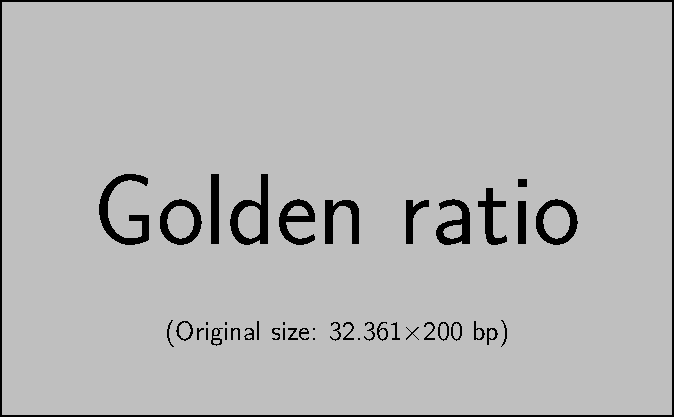
\includegraphics[width=\textwidth]{placeholder_images/example-image-golden.pdf}
    \caption[Schematic illustration depicting geometrical origins of the \gls{spm}]
    {Schematic illustration depicting the geometrical origins of the \gls{spm}. The \gls{spm} is obtained through a degenerate spatial discretisation of one electrochemical layer within a typical Li-ion pouch cell. The axial direction along the cell's thickness is denoted by $x(t)$, whilst the pseudo-dimension along the radial depth of each electrode particle is denoted by $r(t)$. In the basic \gls{spm}, the active material of each porous electrode is represented by one representative spherical particle, thus entirely eliminating the spatial dimension along the axial direction.}
    \label{fig:sandwichtospm}
\end{figure}


Figure~\cref{fig:sandwichtospm}  shows the  arrangement  of one  electrochemical
layer within a typical Li-ion pouch cell. A description of the working principle
of the  cell was presented in~\cref{ch:chapter1}  and is not repeated  here. The
\gls{spm}, as the name suggests,  models the electrochemical phenomena along the
thickness  $l_j$, \jinnegpos{}  of  each porous  electrode  by a  representative
spherical particle.  Thus the two  distinct solid-phase porous materials  of the
cell, \ie{} the  negative and positive electrodes, are idealised  as two spheres
of radii $r_\text{neg}$ and $r_\text{pos}$ respectively.


In  this  reformulated  arrangement,  the  spatial  dimension  along  the  axial
thickness  of  each  electrode  degenerates   to  a  single  point.  Hence,  the
concentration of Lithium within each electrode $c_{\text{s}_j}$, \jinnegpos{} is
only a  function of the radial  position $r_j$, \jinnegpos{} along  the depth of
their  representative  spherical  particle,  and time,  $t$.  The  surface  area
of  each representative  sphere  is  scaled appropriately,  such  that they  are
equivalent  to the  active area  of  the corresponding  porous electrodes.  Thus
the  \gls{spm} accounts  for  the  reduced volume-fraction  arising  due to  the
microporous  structure of  the solid-phase.  The overarching  assumption of  the
\gls{spm} modelling philosophy is that  the electrochemical performance of these
representative electrodes are  sufficient to model the behaviour of  the cell at
its  terminals.  The  \gls{spm}  thus  employs  the  coarsest  possible  spatial
discretisation of the cell's thickness with the goal of minimising computational
burden.


\subsection{Model Development --- Scope and Assumptions}

Having established the geometrical representation of the model, it is imperative
to establish its  aims and scope. This section discusses  the subset of physical
phenomena that can captured by the model and enumerates the inherent assumptions
in  model derivation.The  validity of  these  assumptions and  their effects  is
discussed  in~\cref{subsec:basicspmlimitations}.  As  a  broad  outline  of  the
\gls{spm}s scope,  the model  attributes the cell  polarisation to  two dominant
physics,  \viz{} reaction  kinetics and  solid-phase transport  phenomena, \ie{}
diffusion dynamics.


The gls{spm} assumes that charge transfer happens throughout the surface of each
representative  spherical particle  where intercalation  occurs. The  electronic
conductivity  of the  solid-phase is  assumed to  be high  enough to  ignore the
spatial distribution  of charge, \ie{}  the local volumetric current  density is
assumed  to be  uniform  along  the thickness  of  each  porous electrode.  This
assumption  is motivated  by  the  early calculations  performed  by Newman  and
Tobias~\cite{Newman1962} in their stand-alone  analysis of current distributions
in porous electrodes, wherein a volume-averaged molar flux is deemed sufficient.
This uniform current density assumption implies that all of the particles in the
electrode active material are in parallel.


In the  \gls{spm}, solid-phase  diffusion dynamics are  solved by  assuming this
averaged electrochemical  reaction rate.  In the simulation  study by  Smith and
Wang~\cite{Smith2006b},  it  is  reported  that, soon  after  the  beginning  of
discharge, solid-phase concentration and ionic flux become nearly independent of
spatial position, and  Lithium diffusion in solid particles may  be driven by an
averaged molar flux at the surface.


\subsection{Limitations and Drawbacks}\label{subsec:basicspmlimitations}

The modelling foundations of the \gls{spm} have been






\section{Electrolyte Inclusion}\label{sec:electrolyteinclusion}

Rahimian~\etal{}~\cite{KhaleghiRahimian2013} discuss  the usage of  a polynomial
approximation  for   electrolyte  concentration  and  potentials.   However,  no
restriction was imposed on the order  of the polynomials chosen to represent the
electrolyte concentration within  each porous electrode region.  In the standard
\gls{dfn} model, the  number of equations and  corresponding boundary conditions
describing electrolyte charge and mass transport within the cell is insufficient
to uniquely solve for all  unknown coefficients of the polynomial approximation.
The  challenges  posed  due  to  this equation  deficiency  shall  be  discussed
in~\cref{temp:eqndeficiency}. Although  the original  \gls{spm} did  not involve
solving  for  the  electrolyte  concentrations  or  potentials,  The  polynomial
approximation of the single


Rahimian~\etal{} adopted  a cubic  polynomial for approximating  the electrolyte
concentration within  the porous electrodes.  To overcome the issue  of equation
deficiency, they adapted a scheme wherein one additional spatial location in the
interior  of  each  electrode  was  used. The  coefficients  of  the  polynomial
approximation  were then  obtained  by iteratively  solving  a relatively  large
coupled  system of  algebraic equations,  embedding within  them the  additional
equations evaluated at  the interior point. An additional  complicating issue is
the specific positioning of this  additional interior point. An online numerical
optimisation  was performed  to obtain  the optimal  placement of  this interior
node. Although it serves as a proof of concept towards implementing higher order
polynomial approximations,  the author of this  thesis deems this method  as too
complex for online implementations.

\section{New Electrolyte Model}\label{sec:newelectrolytemodel}



\subsection{equation deficiency \dots}\label{temp:eqndeficiency}

% \begin{figure}[htb]
% \begin{algorithmic}[1]

% \Procedure{SUM}{ $\{x\}$}

% \State $y\gets0$
% \For{$i \gets 1 : N^{x}$} \Comment{Time series $\{x\}$ has length $N^{x}$}
%    \State $y\gets y+x(i)$ \Comment{Summing up.}
% \EndFor

% \State \textbf{return}  $y$
% \EndProcedure
% \end{algorithmic}
% \caption[Implementation of a algorithm for calculating a sum.]{Implementation of a algorithm for calculating a sum.}
% \label{fig:algorithm1}
% \end{figure}




% ---------------------------------------------------------------------------
%: ----------------------- end of thesis sub-document ------------------------
% ---------------------------------------------------------------------------


 % Improved DRA
% -*- root: ../thesis.tex -*-
%!TEX root = ../thesis.tex
% ******************************* Thesis Chapter 5 ****************************


% ----------------------- paths to graphics ------------------------

% change according to folder and file names
\graphicspath{{5/figures/}}
% ----------------------- contents from here ------------------------


\begin{figure}[htb]
  \centering

\resizebox{1\textwidth}{!}{%% Creator: Matplotlib, PGF backend
%%
%% To include the figure in your LaTeX document, write
%%   \input{<filename>.pgf}
%%
%% Make sure the required packages are loaded in your preamble
%%   \usepackage{pgf}
%%
%% Figures using additional raster images can only be included by \input if
%% they are in the same directory as the main LaTeX file. For loading figures
%% from other directories you can use the `import` package
%%   \usepackage{import}
%% and then include the figures with
%%   \import{<path to file>}{<filename>.pgf}
%%
%% Matplotlib used the following preamble
%%   \usepackage{fontspec}
%%   \setmainfont{Times New Roman}
%%   \setsansfont{Verdana}
%%   \setmonofont{Courier New}
%%
\begingroup%
\makeatletter%
\begin{pgfpicture}%
\pgfpathrectangle{\pgfpointorigin}{\pgfqpoint{6.400000in}{4.800000in}}%
\pgfusepath{use as bounding box, clip}%
\begin{pgfscope}%
\pgfsetbuttcap%
\pgfsetmiterjoin%
\definecolor{currentfill}{rgb}{1.000000,1.000000,1.000000}%
\pgfsetfillcolor{currentfill}%
\pgfsetlinewidth{0.000000pt}%
\definecolor{currentstroke}{rgb}{1.000000,1.000000,1.000000}%
\pgfsetstrokecolor{currentstroke}%
\pgfsetdash{}{0pt}%
\pgfpathmoveto{\pgfqpoint{0.000000in}{0.000000in}}%
\pgfpathlineto{\pgfqpoint{6.400000in}{0.000000in}}%
\pgfpathlineto{\pgfqpoint{6.400000in}{4.800000in}}%
\pgfpathlineto{\pgfqpoint{0.000000in}{4.800000in}}%
\pgfpathclose%
\pgfusepath{fill}%
\end{pgfscope}%
\begin{pgfscope}%
\pgfsetbuttcap%
\pgfsetmiterjoin%
\definecolor{currentfill}{rgb}{1.000000,1.000000,1.000000}%
\pgfsetfillcolor{currentfill}%
\pgfsetlinewidth{0.000000pt}%
\definecolor{currentstroke}{rgb}{0.000000,0.000000,0.000000}%
\pgfsetstrokecolor{currentstroke}%
\pgfsetstrokeopacity{0.000000}%
\pgfsetdash{}{0pt}%
\pgfpathmoveto{\pgfqpoint{0.800000in}{0.600000in}}%
\pgfpathlineto{\pgfqpoint{5.888000in}{0.600000in}}%
\pgfpathlineto{\pgfqpoint{5.888000in}{4.320000in}}%
\pgfpathlineto{\pgfqpoint{0.800000in}{4.320000in}}%
\pgfpathclose%
\pgfusepath{fill}%
\end{pgfscope}%
\begin{pgfscope}%
\pgfpathrectangle{\pgfqpoint{0.800000in}{0.600000in}}{\pgfqpoint{5.088000in}{3.720000in}} %
\pgfusepath{clip}%
\pgfsetrectcap%
\pgfsetroundjoin%
\pgfsetlinewidth{0.803000pt}%
\definecolor{currentstroke}{rgb}{0.690196,0.690196,0.690196}%
\pgfsetstrokecolor{currentstroke}%
\pgfsetdash{}{0pt}%
\pgfpathmoveto{\pgfqpoint{0.800000in}{0.600000in}}%
\pgfpathlineto{\pgfqpoint{0.800000in}{4.320000in}}%
\pgfusepath{stroke}%
\end{pgfscope}%
\begin{pgfscope}%
\pgfsetbuttcap%
\pgfsetroundjoin%
\definecolor{currentfill}{rgb}{0.501961,0.501961,0.501961}%
\pgfsetfillcolor{currentfill}%
\pgfsetlinewidth{0.803000pt}%
\definecolor{currentstroke}{rgb}{0.501961,0.501961,0.501961}%
\pgfsetstrokecolor{currentstroke}%
\pgfsetdash{}{0pt}%
\pgfsys@defobject{currentmarker}{\pgfqpoint{0.000000in}{-0.048611in}}{\pgfqpoint{0.000000in}{0.000000in}}{%
\pgfpathmoveto{\pgfqpoint{0.000000in}{0.000000in}}%
\pgfpathlineto{\pgfqpoint{0.000000in}{-0.048611in}}%
\pgfusepath{stroke,fill}%
}%
\begin{pgfscope}%
\pgfsys@transformshift{0.800000in}{0.600000in}%
\pgfsys@useobject{currentmarker}{}%
\end{pgfscope}%
\end{pgfscope}%
\begin{pgfscope}%
\pgftext[x=0.800000in,y=0.502778in,,top]{\sffamily\fontsize{10.000000}{12.000000}\selectfont \(\displaystyle 0.0\)}%
\end{pgfscope}%
\begin{pgfscope}%
\pgfpathrectangle{\pgfqpoint{0.800000in}{0.600000in}}{\pgfqpoint{5.088000in}{3.720000in}} %
\pgfusepath{clip}%
\pgfsetrectcap%
\pgfsetroundjoin%
\pgfsetlinewidth{0.803000pt}%
\definecolor{currentstroke}{rgb}{0.690196,0.690196,0.690196}%
\pgfsetstrokecolor{currentstroke}%
\pgfsetdash{}{0pt}%
\pgfpathmoveto{\pgfqpoint{1.817600in}{0.600000in}}%
\pgfpathlineto{\pgfqpoint{1.817600in}{4.320000in}}%
\pgfusepath{stroke}%
\end{pgfscope}%
\begin{pgfscope}%
\pgfsetbuttcap%
\pgfsetroundjoin%
\definecolor{currentfill}{rgb}{0.501961,0.501961,0.501961}%
\pgfsetfillcolor{currentfill}%
\pgfsetlinewidth{0.803000pt}%
\definecolor{currentstroke}{rgb}{0.501961,0.501961,0.501961}%
\pgfsetstrokecolor{currentstroke}%
\pgfsetdash{}{0pt}%
\pgfsys@defobject{currentmarker}{\pgfqpoint{0.000000in}{-0.048611in}}{\pgfqpoint{0.000000in}{0.000000in}}{%
\pgfpathmoveto{\pgfqpoint{0.000000in}{0.000000in}}%
\pgfpathlineto{\pgfqpoint{0.000000in}{-0.048611in}}%
\pgfusepath{stroke,fill}%
}%
\begin{pgfscope}%
\pgfsys@transformshift{1.817600in}{0.600000in}%
\pgfsys@useobject{currentmarker}{}%
\end{pgfscope}%
\end{pgfscope}%
\begin{pgfscope}%
\pgftext[x=1.817600in,y=0.502778in,,top]{\sffamily\fontsize{10.000000}{12.000000}\selectfont \(\displaystyle 0.2\)}%
\end{pgfscope}%
\begin{pgfscope}%
\pgfpathrectangle{\pgfqpoint{0.800000in}{0.600000in}}{\pgfqpoint{5.088000in}{3.720000in}} %
\pgfusepath{clip}%
\pgfsetrectcap%
\pgfsetroundjoin%
\pgfsetlinewidth{0.803000pt}%
\definecolor{currentstroke}{rgb}{0.690196,0.690196,0.690196}%
\pgfsetstrokecolor{currentstroke}%
\pgfsetdash{}{0pt}%
\pgfpathmoveto{\pgfqpoint{2.835200in}{0.600000in}}%
\pgfpathlineto{\pgfqpoint{2.835200in}{4.320000in}}%
\pgfusepath{stroke}%
\end{pgfscope}%
\begin{pgfscope}%
\pgfsetbuttcap%
\pgfsetroundjoin%
\definecolor{currentfill}{rgb}{0.501961,0.501961,0.501961}%
\pgfsetfillcolor{currentfill}%
\pgfsetlinewidth{0.803000pt}%
\definecolor{currentstroke}{rgb}{0.501961,0.501961,0.501961}%
\pgfsetstrokecolor{currentstroke}%
\pgfsetdash{}{0pt}%
\pgfsys@defobject{currentmarker}{\pgfqpoint{0.000000in}{-0.048611in}}{\pgfqpoint{0.000000in}{0.000000in}}{%
\pgfpathmoveto{\pgfqpoint{0.000000in}{0.000000in}}%
\pgfpathlineto{\pgfqpoint{0.000000in}{-0.048611in}}%
\pgfusepath{stroke,fill}%
}%
\begin{pgfscope}%
\pgfsys@transformshift{2.835200in}{0.600000in}%
\pgfsys@useobject{currentmarker}{}%
\end{pgfscope}%
\end{pgfscope}%
\begin{pgfscope}%
\pgftext[x=2.835200in,y=0.502778in,,top]{\sffamily\fontsize{10.000000}{12.000000}\selectfont \(\displaystyle 0.4\)}%
\end{pgfscope}%
\begin{pgfscope}%
\pgfpathrectangle{\pgfqpoint{0.800000in}{0.600000in}}{\pgfqpoint{5.088000in}{3.720000in}} %
\pgfusepath{clip}%
\pgfsetrectcap%
\pgfsetroundjoin%
\pgfsetlinewidth{0.803000pt}%
\definecolor{currentstroke}{rgb}{0.690196,0.690196,0.690196}%
\pgfsetstrokecolor{currentstroke}%
\pgfsetdash{}{0pt}%
\pgfpathmoveto{\pgfqpoint{3.852800in}{0.600000in}}%
\pgfpathlineto{\pgfqpoint{3.852800in}{4.320000in}}%
\pgfusepath{stroke}%
\end{pgfscope}%
\begin{pgfscope}%
\pgfsetbuttcap%
\pgfsetroundjoin%
\definecolor{currentfill}{rgb}{0.501961,0.501961,0.501961}%
\pgfsetfillcolor{currentfill}%
\pgfsetlinewidth{0.803000pt}%
\definecolor{currentstroke}{rgb}{0.501961,0.501961,0.501961}%
\pgfsetstrokecolor{currentstroke}%
\pgfsetdash{}{0pt}%
\pgfsys@defobject{currentmarker}{\pgfqpoint{0.000000in}{-0.048611in}}{\pgfqpoint{0.000000in}{0.000000in}}{%
\pgfpathmoveto{\pgfqpoint{0.000000in}{0.000000in}}%
\pgfpathlineto{\pgfqpoint{0.000000in}{-0.048611in}}%
\pgfusepath{stroke,fill}%
}%
\begin{pgfscope}%
\pgfsys@transformshift{3.852800in}{0.600000in}%
\pgfsys@useobject{currentmarker}{}%
\end{pgfscope}%
\end{pgfscope}%
\begin{pgfscope}%
\pgftext[x=3.852800in,y=0.502778in,,top]{\sffamily\fontsize{10.000000}{12.000000}\selectfont \(\displaystyle 0.6\)}%
\end{pgfscope}%
\begin{pgfscope}%
\pgfpathrectangle{\pgfqpoint{0.800000in}{0.600000in}}{\pgfqpoint{5.088000in}{3.720000in}} %
\pgfusepath{clip}%
\pgfsetrectcap%
\pgfsetroundjoin%
\pgfsetlinewidth{0.803000pt}%
\definecolor{currentstroke}{rgb}{0.690196,0.690196,0.690196}%
\pgfsetstrokecolor{currentstroke}%
\pgfsetdash{}{0pt}%
\pgfpathmoveto{\pgfqpoint{4.870400in}{0.600000in}}%
\pgfpathlineto{\pgfqpoint{4.870400in}{4.320000in}}%
\pgfusepath{stroke}%
\end{pgfscope}%
\begin{pgfscope}%
\pgfsetbuttcap%
\pgfsetroundjoin%
\definecolor{currentfill}{rgb}{0.501961,0.501961,0.501961}%
\pgfsetfillcolor{currentfill}%
\pgfsetlinewidth{0.803000pt}%
\definecolor{currentstroke}{rgb}{0.501961,0.501961,0.501961}%
\pgfsetstrokecolor{currentstroke}%
\pgfsetdash{}{0pt}%
\pgfsys@defobject{currentmarker}{\pgfqpoint{0.000000in}{-0.048611in}}{\pgfqpoint{0.000000in}{0.000000in}}{%
\pgfpathmoveto{\pgfqpoint{0.000000in}{0.000000in}}%
\pgfpathlineto{\pgfqpoint{0.000000in}{-0.048611in}}%
\pgfusepath{stroke,fill}%
}%
\begin{pgfscope}%
\pgfsys@transformshift{4.870400in}{0.600000in}%
\pgfsys@useobject{currentmarker}{}%
\end{pgfscope}%
\end{pgfscope}%
\begin{pgfscope}%
\pgftext[x=4.870400in,y=0.502778in,,top]{\sffamily\fontsize{10.000000}{12.000000}\selectfont \(\displaystyle 0.8\)}%
\end{pgfscope}%
\begin{pgfscope}%
\pgfpathrectangle{\pgfqpoint{0.800000in}{0.600000in}}{\pgfqpoint{5.088000in}{3.720000in}} %
\pgfusepath{clip}%
\pgfsetrectcap%
\pgfsetroundjoin%
\pgfsetlinewidth{0.803000pt}%
\definecolor{currentstroke}{rgb}{0.690196,0.690196,0.690196}%
\pgfsetstrokecolor{currentstroke}%
\pgfsetdash{}{0pt}%
\pgfpathmoveto{\pgfqpoint{5.888000in}{0.600000in}}%
\pgfpathlineto{\pgfqpoint{5.888000in}{4.320000in}}%
\pgfusepath{stroke}%
\end{pgfscope}%
\begin{pgfscope}%
\pgfsetbuttcap%
\pgfsetroundjoin%
\definecolor{currentfill}{rgb}{0.501961,0.501961,0.501961}%
\pgfsetfillcolor{currentfill}%
\pgfsetlinewidth{0.803000pt}%
\definecolor{currentstroke}{rgb}{0.501961,0.501961,0.501961}%
\pgfsetstrokecolor{currentstroke}%
\pgfsetdash{}{0pt}%
\pgfsys@defobject{currentmarker}{\pgfqpoint{0.000000in}{-0.048611in}}{\pgfqpoint{0.000000in}{0.000000in}}{%
\pgfpathmoveto{\pgfqpoint{0.000000in}{0.000000in}}%
\pgfpathlineto{\pgfqpoint{0.000000in}{-0.048611in}}%
\pgfusepath{stroke,fill}%
}%
\begin{pgfscope}%
\pgfsys@transformshift{5.888000in}{0.600000in}%
\pgfsys@useobject{currentmarker}{}%
\end{pgfscope}%
\end{pgfscope}%
\begin{pgfscope}%
\pgftext[x=5.888000in,y=0.502778in,,top]{\sffamily\fontsize{10.000000}{12.000000}\selectfont \(\displaystyle 1.0\)}%
\end{pgfscope}%
\begin{pgfscope}%
\pgftext[x=3.344000in,y=0.313759in,,top]{\sffamily\fontsize{10.000000}{12.000000}\selectfont False positive rate}%
\end{pgfscope}%
\begin{pgfscope}%
\pgfpathrectangle{\pgfqpoint{0.800000in}{0.600000in}}{\pgfqpoint{5.088000in}{3.720000in}} %
\pgfusepath{clip}%
\pgfsetrectcap%
\pgfsetroundjoin%
\pgfsetlinewidth{0.803000pt}%
\definecolor{currentstroke}{rgb}{0.690196,0.690196,0.690196}%
\pgfsetstrokecolor{currentstroke}%
\pgfsetdash{}{0pt}%
\pgfpathmoveto{\pgfqpoint{0.800000in}{0.600000in}}%
\pgfpathlineto{\pgfqpoint{5.888000in}{0.600000in}}%
\pgfusepath{stroke}%
\end{pgfscope}%
\begin{pgfscope}%
\pgfsetbuttcap%
\pgfsetroundjoin%
\definecolor{currentfill}{rgb}{0.501961,0.501961,0.501961}%
\pgfsetfillcolor{currentfill}%
\pgfsetlinewidth{0.803000pt}%
\definecolor{currentstroke}{rgb}{0.501961,0.501961,0.501961}%
\pgfsetstrokecolor{currentstroke}%
\pgfsetdash{}{0pt}%
\pgfsys@defobject{currentmarker}{\pgfqpoint{-0.048611in}{0.000000in}}{\pgfqpoint{0.000000in}{0.000000in}}{%
\pgfpathmoveto{\pgfqpoint{0.000000in}{0.000000in}}%
\pgfpathlineto{\pgfqpoint{-0.048611in}{0.000000in}}%
\pgfusepath{stroke,fill}%
}%
\begin{pgfscope}%
\pgfsys@transformshift{0.800000in}{0.600000in}%
\pgfsys@useobject{currentmarker}{}%
\end{pgfscope}%
\end{pgfscope}%
\begin{pgfscope}%
\pgftext[x=0.525308in,y=0.547238in,left,base]{\sffamily\fontsize{10.000000}{12.000000}\selectfont \(\displaystyle 0.0\)}%
\end{pgfscope}%
\begin{pgfscope}%
\pgfpathrectangle{\pgfqpoint{0.800000in}{0.600000in}}{\pgfqpoint{5.088000in}{3.720000in}} %
\pgfusepath{clip}%
\pgfsetrectcap%
\pgfsetroundjoin%
\pgfsetlinewidth{0.803000pt}%
\definecolor{currentstroke}{rgb}{0.690196,0.690196,0.690196}%
\pgfsetstrokecolor{currentstroke}%
\pgfsetdash{}{0pt}%
\pgfpathmoveto{\pgfqpoint{0.800000in}{1.344000in}}%
\pgfpathlineto{\pgfqpoint{5.888000in}{1.344000in}}%
\pgfusepath{stroke}%
\end{pgfscope}%
\begin{pgfscope}%
\pgfsetbuttcap%
\pgfsetroundjoin%
\definecolor{currentfill}{rgb}{0.501961,0.501961,0.501961}%
\pgfsetfillcolor{currentfill}%
\pgfsetlinewidth{0.803000pt}%
\definecolor{currentstroke}{rgb}{0.501961,0.501961,0.501961}%
\pgfsetstrokecolor{currentstroke}%
\pgfsetdash{}{0pt}%
\pgfsys@defobject{currentmarker}{\pgfqpoint{-0.048611in}{0.000000in}}{\pgfqpoint{0.000000in}{0.000000in}}{%
\pgfpathmoveto{\pgfqpoint{0.000000in}{0.000000in}}%
\pgfpathlineto{\pgfqpoint{-0.048611in}{0.000000in}}%
\pgfusepath{stroke,fill}%
}%
\begin{pgfscope}%
\pgfsys@transformshift{0.800000in}{1.344000in}%
\pgfsys@useobject{currentmarker}{}%
\end{pgfscope}%
\end{pgfscope}%
\begin{pgfscope}%
\pgftext[x=0.525308in,y=1.291238in,left,base]{\sffamily\fontsize{10.000000}{12.000000}\selectfont \(\displaystyle 0.2\)}%
\end{pgfscope}%
\begin{pgfscope}%
\pgfpathrectangle{\pgfqpoint{0.800000in}{0.600000in}}{\pgfqpoint{5.088000in}{3.720000in}} %
\pgfusepath{clip}%
\pgfsetrectcap%
\pgfsetroundjoin%
\pgfsetlinewidth{0.803000pt}%
\definecolor{currentstroke}{rgb}{0.690196,0.690196,0.690196}%
\pgfsetstrokecolor{currentstroke}%
\pgfsetdash{}{0pt}%
\pgfpathmoveto{\pgfqpoint{0.800000in}{2.088000in}}%
\pgfpathlineto{\pgfqpoint{5.888000in}{2.088000in}}%
\pgfusepath{stroke}%
\end{pgfscope}%
\begin{pgfscope}%
\pgfsetbuttcap%
\pgfsetroundjoin%
\definecolor{currentfill}{rgb}{0.501961,0.501961,0.501961}%
\pgfsetfillcolor{currentfill}%
\pgfsetlinewidth{0.803000pt}%
\definecolor{currentstroke}{rgb}{0.501961,0.501961,0.501961}%
\pgfsetstrokecolor{currentstroke}%
\pgfsetdash{}{0pt}%
\pgfsys@defobject{currentmarker}{\pgfqpoint{-0.048611in}{0.000000in}}{\pgfqpoint{0.000000in}{0.000000in}}{%
\pgfpathmoveto{\pgfqpoint{0.000000in}{0.000000in}}%
\pgfpathlineto{\pgfqpoint{-0.048611in}{0.000000in}}%
\pgfusepath{stroke,fill}%
}%
\begin{pgfscope}%
\pgfsys@transformshift{0.800000in}{2.088000in}%
\pgfsys@useobject{currentmarker}{}%
\end{pgfscope}%
\end{pgfscope}%
\begin{pgfscope}%
\pgftext[x=0.525308in,y=2.035238in,left,base]{\sffamily\fontsize{10.000000}{12.000000}\selectfont \(\displaystyle 0.4\)}%
\end{pgfscope}%
\begin{pgfscope}%
\pgfpathrectangle{\pgfqpoint{0.800000in}{0.600000in}}{\pgfqpoint{5.088000in}{3.720000in}} %
\pgfusepath{clip}%
\pgfsetrectcap%
\pgfsetroundjoin%
\pgfsetlinewidth{0.803000pt}%
\definecolor{currentstroke}{rgb}{0.690196,0.690196,0.690196}%
\pgfsetstrokecolor{currentstroke}%
\pgfsetdash{}{0pt}%
\pgfpathmoveto{\pgfqpoint{0.800000in}{2.832000in}}%
\pgfpathlineto{\pgfqpoint{5.888000in}{2.832000in}}%
\pgfusepath{stroke}%
\end{pgfscope}%
\begin{pgfscope}%
\pgfsetbuttcap%
\pgfsetroundjoin%
\definecolor{currentfill}{rgb}{0.501961,0.501961,0.501961}%
\pgfsetfillcolor{currentfill}%
\pgfsetlinewidth{0.803000pt}%
\definecolor{currentstroke}{rgb}{0.501961,0.501961,0.501961}%
\pgfsetstrokecolor{currentstroke}%
\pgfsetdash{}{0pt}%
\pgfsys@defobject{currentmarker}{\pgfqpoint{-0.048611in}{0.000000in}}{\pgfqpoint{0.000000in}{0.000000in}}{%
\pgfpathmoveto{\pgfqpoint{0.000000in}{0.000000in}}%
\pgfpathlineto{\pgfqpoint{-0.048611in}{0.000000in}}%
\pgfusepath{stroke,fill}%
}%
\begin{pgfscope}%
\pgfsys@transformshift{0.800000in}{2.832000in}%
\pgfsys@useobject{currentmarker}{}%
\end{pgfscope}%
\end{pgfscope}%
\begin{pgfscope}%
\pgftext[x=0.525308in,y=2.779238in,left,base]{\sffamily\fontsize{10.000000}{12.000000}\selectfont \(\displaystyle 0.6\)}%
\end{pgfscope}%
\begin{pgfscope}%
\pgfpathrectangle{\pgfqpoint{0.800000in}{0.600000in}}{\pgfqpoint{5.088000in}{3.720000in}} %
\pgfusepath{clip}%
\pgfsetrectcap%
\pgfsetroundjoin%
\pgfsetlinewidth{0.803000pt}%
\definecolor{currentstroke}{rgb}{0.690196,0.690196,0.690196}%
\pgfsetstrokecolor{currentstroke}%
\pgfsetdash{}{0pt}%
\pgfpathmoveto{\pgfqpoint{0.800000in}{3.576000in}}%
\pgfpathlineto{\pgfqpoint{5.888000in}{3.576000in}}%
\pgfusepath{stroke}%
\end{pgfscope}%
\begin{pgfscope}%
\pgfsetbuttcap%
\pgfsetroundjoin%
\definecolor{currentfill}{rgb}{0.501961,0.501961,0.501961}%
\pgfsetfillcolor{currentfill}%
\pgfsetlinewidth{0.803000pt}%
\definecolor{currentstroke}{rgb}{0.501961,0.501961,0.501961}%
\pgfsetstrokecolor{currentstroke}%
\pgfsetdash{}{0pt}%
\pgfsys@defobject{currentmarker}{\pgfqpoint{-0.048611in}{0.000000in}}{\pgfqpoint{0.000000in}{0.000000in}}{%
\pgfpathmoveto{\pgfqpoint{0.000000in}{0.000000in}}%
\pgfpathlineto{\pgfqpoint{-0.048611in}{0.000000in}}%
\pgfusepath{stroke,fill}%
}%
\begin{pgfscope}%
\pgfsys@transformshift{0.800000in}{3.576000in}%
\pgfsys@useobject{currentmarker}{}%
\end{pgfscope}%
\end{pgfscope}%
\begin{pgfscope}%
\pgftext[x=0.525308in,y=3.523238in,left,base]{\sffamily\fontsize{10.000000}{12.000000}\selectfont \(\displaystyle 0.8\)}%
\end{pgfscope}%
\begin{pgfscope}%
\pgfpathrectangle{\pgfqpoint{0.800000in}{0.600000in}}{\pgfqpoint{5.088000in}{3.720000in}} %
\pgfusepath{clip}%
\pgfsetrectcap%
\pgfsetroundjoin%
\pgfsetlinewidth{0.803000pt}%
\definecolor{currentstroke}{rgb}{0.690196,0.690196,0.690196}%
\pgfsetstrokecolor{currentstroke}%
\pgfsetdash{}{0pt}%
\pgfpathmoveto{\pgfqpoint{0.800000in}{4.320000in}}%
\pgfpathlineto{\pgfqpoint{5.888000in}{4.320000in}}%
\pgfusepath{stroke}%
\end{pgfscope}%
\begin{pgfscope}%
\pgfsetbuttcap%
\pgfsetroundjoin%
\definecolor{currentfill}{rgb}{0.501961,0.501961,0.501961}%
\pgfsetfillcolor{currentfill}%
\pgfsetlinewidth{0.803000pt}%
\definecolor{currentstroke}{rgb}{0.501961,0.501961,0.501961}%
\pgfsetstrokecolor{currentstroke}%
\pgfsetdash{}{0pt}%
\pgfsys@defobject{currentmarker}{\pgfqpoint{-0.048611in}{0.000000in}}{\pgfqpoint{0.000000in}{0.000000in}}{%
\pgfpathmoveto{\pgfqpoint{0.000000in}{0.000000in}}%
\pgfpathlineto{\pgfqpoint{-0.048611in}{0.000000in}}%
\pgfusepath{stroke,fill}%
}%
\begin{pgfscope}%
\pgfsys@transformshift{0.800000in}{4.320000in}%
\pgfsys@useobject{currentmarker}{}%
\end{pgfscope}%
\end{pgfscope}%
\begin{pgfscope}%
\pgftext[x=0.525308in,y=4.267238in,left,base]{\sffamily\fontsize{10.000000}{12.000000}\selectfont \(\displaystyle 1.0\)}%
\end{pgfscope}%
\begin{pgfscope}%
\pgftext[x=0.469753in,y=2.460000in,,bottom,rotate=90.000000]{\sffamily\fontsize{10.000000}{12.000000}\selectfont True positive rate}%
\end{pgfscope}%
\begin{pgfscope}%
\pgfpathrectangle{\pgfqpoint{0.800000in}{0.600000in}}{\pgfqpoint{5.088000in}{3.720000in}} %
\pgfusepath{clip}%
\pgfsetrectcap%
\pgfsetroundjoin%
\pgfsetlinewidth{1.505625pt}%
\definecolor{currentstroke}{rgb}{0.121569,0.470588,0.705882}%
\pgfsetstrokecolor{currentstroke}%
\pgfsetdash{}{0pt}%
\pgfpathmoveto{\pgfqpoint{0.800000in}{0.600000in}}%
\pgfpathlineto{\pgfqpoint{0.806368in}{0.978981in}}%
\pgfpathlineto{\pgfqpoint{0.831840in}{1.118606in}}%
\pgfpathlineto{\pgfqpoint{0.844576in}{1.148525in}}%
\pgfpathlineto{\pgfqpoint{0.850944in}{1.308097in}}%
\pgfpathlineto{\pgfqpoint{0.876416in}{1.607292in}}%
\pgfpathlineto{\pgfqpoint{0.882783in}{1.627239in}}%
\pgfpathlineto{\pgfqpoint{0.920991in}{1.816729in}}%
\pgfpathlineto{\pgfqpoint{1.022879in}{1.936408in}}%
\pgfpathlineto{\pgfqpoint{1.041982in}{1.946381in}}%
\pgfpathlineto{\pgfqpoint{1.054718in}{1.976300in}}%
\pgfpathlineto{\pgfqpoint{1.061086in}{2.036139in}}%
\pgfpathlineto{\pgfqpoint{1.131134in}{2.514853in}}%
\pgfpathlineto{\pgfqpoint{1.207549in}{2.863914in}}%
\pgfpathlineto{\pgfqpoint{1.220285in}{2.863914in}}%
\pgfpathlineto{\pgfqpoint{1.233021in}{2.953673in}}%
\pgfpathlineto{\pgfqpoint{1.233021in}{2.983592in}}%
\pgfpathlineto{\pgfqpoint{1.245757in}{2.983592in}}%
\pgfpathlineto{\pgfqpoint{1.252125in}{2.993566in}}%
\pgfpathlineto{\pgfqpoint{1.252125in}{3.003539in}}%
\pgfpathlineto{\pgfqpoint{1.264861in}{3.163110in}}%
\pgfpathlineto{\pgfqpoint{1.271229in}{3.163110in}}%
\pgfpathlineto{\pgfqpoint{1.309437in}{3.252869in}}%
\pgfpathlineto{\pgfqpoint{1.328541in}{3.322681in}}%
\pgfpathlineto{\pgfqpoint{1.341277in}{3.322681in}}%
\pgfpathlineto{\pgfqpoint{1.430428in}{3.372547in}}%
\pgfpathlineto{\pgfqpoint{1.436796in}{3.372547in}}%
\pgfpathlineto{\pgfqpoint{1.449532in}{3.442359in}}%
\pgfpathlineto{\pgfqpoint{1.494108in}{3.532118in}}%
\pgfpathlineto{\pgfqpoint{1.500476in}{3.542091in}}%
\pgfpathlineto{\pgfqpoint{1.506844in}{3.542091in}}%
\pgfpathlineto{\pgfqpoint{1.519579in}{3.552064in}}%
\pgfpathlineto{\pgfqpoint{1.576891in}{3.552064in}}%
\pgfpathlineto{\pgfqpoint{1.576891in}{3.581984in}}%
\pgfpathlineto{\pgfqpoint{1.583259in}{3.581984in}}%
\pgfpathlineto{\pgfqpoint{1.595995in}{3.741555in}}%
\pgfpathlineto{\pgfqpoint{1.608731in}{3.771475in}}%
\pgfpathlineto{\pgfqpoint{1.615099in}{3.771475in}}%
\pgfpathlineto{\pgfqpoint{1.653307in}{3.791421in}}%
\pgfpathlineto{\pgfqpoint{1.685146in}{3.791421in}}%
\pgfpathlineto{\pgfqpoint{1.697882in}{3.801394in}}%
\pgfpathlineto{\pgfqpoint{1.710618in}{3.801394in}}%
\pgfpathlineto{\pgfqpoint{1.710618in}{3.811367in}}%
\pgfpathlineto{\pgfqpoint{1.882553in}{3.811367in}}%
\pgfpathlineto{\pgfqpoint{1.888921in}{3.821340in}}%
\pgfpathlineto{\pgfqpoint{1.888921in}{3.831314in}}%
\pgfpathlineto{\pgfqpoint{1.901657in}{3.831314in}}%
\pgfpathlineto{\pgfqpoint{1.914393in}{3.841287in}}%
\pgfpathlineto{\pgfqpoint{2.003544in}{3.841287in}}%
\pgfpathlineto{\pgfqpoint{2.054488in}{3.891153in}}%
\pgfpathlineto{\pgfqpoint{2.130904in}{3.891153in}}%
\pgfpathlineto{\pgfqpoint{2.175479in}{3.901126in}}%
\pgfpathlineto{\pgfqpoint{2.239159in}{3.901126in}}%
\pgfpathlineto{\pgfqpoint{2.277367in}{3.921072in}}%
\pgfpathlineto{\pgfqpoint{2.468406in}{3.921072in}}%
\pgfpathlineto{\pgfqpoint{2.506613in}{3.931046in}}%
\pgfpathlineto{\pgfqpoint{2.544821in}{3.931046in}}%
\pgfpathlineto{\pgfqpoint{2.602133in}{3.960965in}}%
\pgfpathlineto{\pgfqpoint{2.754964in}{3.960965in}}%
\pgfpathlineto{\pgfqpoint{2.761332in}{3.970938in}}%
\pgfpathlineto{\pgfqpoint{2.786804in}{3.970938in}}%
\pgfpathlineto{\pgfqpoint{2.818643in}{3.980912in}}%
\pgfpathlineto{\pgfqpoint{2.831379in}{3.980912in}}%
\pgfpathlineto{\pgfqpoint{2.856851in}{4.000858in}}%
\pgfpathlineto{\pgfqpoint{2.863219in}{4.010831in}}%
\pgfpathlineto{\pgfqpoint{2.895059in}{4.020804in}}%
\pgfpathlineto{\pgfqpoint{3.105202in}{4.020804in}}%
\pgfpathlineto{\pgfqpoint{3.117937in}{4.030777in}}%
\pgfpathlineto{\pgfqpoint{3.124305in}{4.110563in}}%
\pgfpathlineto{\pgfqpoint{3.404496in}{4.110563in}}%
\pgfpathlineto{\pgfqpoint{3.429967in}{4.210295in}}%
\pgfpathlineto{\pgfqpoint{3.691054in}{4.210295in}}%
\pgfpathlineto{\pgfqpoint{3.697422in}{4.220268in}}%
\pgfpathlineto{\pgfqpoint{4.015820in}{4.220268in}}%
\pgfpathlineto{\pgfqpoint{4.028556in}{4.230241in}}%
\pgfpathlineto{\pgfqpoint{4.175019in}{4.230241in}}%
\pgfpathlineto{\pgfqpoint{4.187755in}{4.240214in}}%
\pgfpathlineto{\pgfqpoint{4.531625in}{4.240214in}}%
\pgfpathlineto{\pgfqpoint{4.569832in}{4.280107in}}%
\pgfpathlineto{\pgfqpoint{4.620776in}{4.280107in}}%
\pgfpathlineto{\pgfqpoint{4.627144in}{4.290080in}}%
\pgfpathlineto{\pgfqpoint{4.830919in}{4.290080in}}%
\pgfpathlineto{\pgfqpoint{4.856390in}{4.300054in}}%
\pgfpathlineto{\pgfqpoint{5.111109in}{4.300054in}}%
\pgfpathlineto{\pgfqpoint{5.130213in}{4.310027in}}%
\pgfpathlineto{\pgfqpoint{5.703329in}{4.310027in}}%
\pgfpathlineto{\pgfqpoint{5.709697in}{4.320000in}}%
\pgfpathlineto{\pgfqpoint{5.888000in}{4.320000in}}%
\pgfpathlineto{\pgfqpoint{5.888000in}{4.320000in}}%
\pgfusepath{stroke}%
\end{pgfscope}%
\begin{pgfscope}%
\pgfpathrectangle{\pgfqpoint{0.800000in}{0.600000in}}{\pgfqpoint{5.088000in}{3.720000in}} %
\pgfusepath{clip}%
\pgfsetbuttcap%
\pgfsetroundjoin%
\pgfsetlinewidth{1.505625pt}%
\definecolor{currentstroke}{rgb}{0.890196,0.101961,0.109804}%
\pgfsetstrokecolor{currentstroke}%
\pgfsetdash{{5.550000pt}{2.400000pt}}{0.000000pt}%
\pgfpathmoveto{\pgfqpoint{0.800000in}{0.600000in}}%
\pgfpathlineto{\pgfqpoint{0.851394in}{0.637576in}}%
\pgfpathlineto{\pgfqpoint{0.902788in}{0.675152in}}%
\pgfpathlineto{\pgfqpoint{0.954182in}{0.712727in}}%
\pgfpathlineto{\pgfqpoint{1.005576in}{0.750303in}}%
\pgfpathlineto{\pgfqpoint{1.056970in}{0.787879in}}%
\pgfpathlineto{\pgfqpoint{1.108364in}{0.825455in}}%
\pgfpathlineto{\pgfqpoint{1.159758in}{0.863030in}}%
\pgfpathlineto{\pgfqpoint{1.211152in}{0.900606in}}%
\pgfpathlineto{\pgfqpoint{1.262545in}{0.938182in}}%
\pgfpathlineto{\pgfqpoint{1.313939in}{0.975758in}}%
\pgfpathlineto{\pgfqpoint{1.365333in}{1.013333in}}%
\pgfpathlineto{\pgfqpoint{1.416727in}{1.050909in}}%
\pgfpathlineto{\pgfqpoint{1.468121in}{1.088485in}}%
\pgfpathlineto{\pgfqpoint{1.519515in}{1.126061in}}%
\pgfpathlineto{\pgfqpoint{1.570909in}{1.163636in}}%
\pgfpathlineto{\pgfqpoint{1.622303in}{1.201212in}}%
\pgfpathlineto{\pgfqpoint{1.673697in}{1.238788in}}%
\pgfpathlineto{\pgfqpoint{1.725091in}{1.276364in}}%
\pgfpathlineto{\pgfqpoint{1.776485in}{1.313939in}}%
\pgfpathlineto{\pgfqpoint{1.827879in}{1.351515in}}%
\pgfpathlineto{\pgfqpoint{1.879273in}{1.389091in}}%
\pgfpathlineto{\pgfqpoint{1.930667in}{1.426667in}}%
\pgfpathlineto{\pgfqpoint{1.982061in}{1.464242in}}%
\pgfpathlineto{\pgfqpoint{2.033455in}{1.501818in}}%
\pgfpathlineto{\pgfqpoint{2.084848in}{1.539394in}}%
\pgfpathlineto{\pgfqpoint{2.136242in}{1.576970in}}%
\pgfpathlineto{\pgfqpoint{2.187636in}{1.614545in}}%
\pgfpathlineto{\pgfqpoint{2.239030in}{1.652121in}}%
\pgfpathlineto{\pgfqpoint{2.290424in}{1.689697in}}%
\pgfpathlineto{\pgfqpoint{2.341818in}{1.727273in}}%
\pgfpathlineto{\pgfqpoint{2.393212in}{1.764848in}}%
\pgfpathlineto{\pgfqpoint{2.444606in}{1.802424in}}%
\pgfpathlineto{\pgfqpoint{2.496000in}{1.840000in}}%
\pgfpathlineto{\pgfqpoint{2.547394in}{1.877576in}}%
\pgfpathlineto{\pgfqpoint{2.598788in}{1.915152in}}%
\pgfpathlineto{\pgfqpoint{2.650182in}{1.952727in}}%
\pgfpathlineto{\pgfqpoint{2.701576in}{1.990303in}}%
\pgfpathlineto{\pgfqpoint{2.752970in}{2.027879in}}%
\pgfpathlineto{\pgfqpoint{2.804364in}{2.065455in}}%
\pgfpathlineto{\pgfqpoint{2.855758in}{2.103030in}}%
\pgfpathlineto{\pgfqpoint{2.907152in}{2.140606in}}%
\pgfpathlineto{\pgfqpoint{2.958545in}{2.178182in}}%
\pgfpathlineto{\pgfqpoint{3.009939in}{2.215758in}}%
\pgfpathlineto{\pgfqpoint{3.061333in}{2.253333in}}%
\pgfpathlineto{\pgfqpoint{3.112727in}{2.290909in}}%
\pgfpathlineto{\pgfqpoint{3.164121in}{2.328485in}}%
\pgfpathlineto{\pgfqpoint{3.215515in}{2.366061in}}%
\pgfpathlineto{\pgfqpoint{3.266909in}{2.403636in}}%
\pgfpathlineto{\pgfqpoint{3.318303in}{2.441212in}}%
\pgfpathlineto{\pgfqpoint{3.369697in}{2.478788in}}%
\pgfpathlineto{\pgfqpoint{3.421091in}{2.516364in}}%
\pgfpathlineto{\pgfqpoint{3.472485in}{2.553939in}}%
\pgfpathlineto{\pgfqpoint{3.523879in}{2.591515in}}%
\pgfpathlineto{\pgfqpoint{3.575273in}{2.629091in}}%
\pgfpathlineto{\pgfqpoint{3.626667in}{2.666667in}}%
\pgfpathlineto{\pgfqpoint{3.678061in}{2.704242in}}%
\pgfpathlineto{\pgfqpoint{3.729455in}{2.741818in}}%
\pgfpathlineto{\pgfqpoint{3.780848in}{2.779394in}}%
\pgfpathlineto{\pgfqpoint{3.832242in}{2.816970in}}%
\pgfpathlineto{\pgfqpoint{3.883636in}{2.854545in}}%
\pgfpathlineto{\pgfqpoint{3.935030in}{2.892121in}}%
\pgfpathlineto{\pgfqpoint{3.986424in}{2.929697in}}%
\pgfpathlineto{\pgfqpoint{4.037818in}{2.967273in}}%
\pgfpathlineto{\pgfqpoint{4.089212in}{3.004848in}}%
\pgfpathlineto{\pgfqpoint{4.140606in}{3.042424in}}%
\pgfpathlineto{\pgfqpoint{4.192000in}{3.080000in}}%
\pgfpathlineto{\pgfqpoint{4.243394in}{3.117576in}}%
\pgfpathlineto{\pgfqpoint{4.294788in}{3.155152in}}%
\pgfpathlineto{\pgfqpoint{4.346182in}{3.192727in}}%
\pgfpathlineto{\pgfqpoint{4.397576in}{3.230303in}}%
\pgfpathlineto{\pgfqpoint{4.448970in}{3.267879in}}%
\pgfpathlineto{\pgfqpoint{4.500364in}{3.305455in}}%
\pgfpathlineto{\pgfqpoint{4.551758in}{3.343030in}}%
\pgfpathlineto{\pgfqpoint{4.603152in}{3.380606in}}%
\pgfpathlineto{\pgfqpoint{4.654545in}{3.418182in}}%
\pgfpathlineto{\pgfqpoint{4.705939in}{3.455758in}}%
\pgfpathlineto{\pgfqpoint{4.757333in}{3.493333in}}%
\pgfpathlineto{\pgfqpoint{4.808727in}{3.530909in}}%
\pgfpathlineto{\pgfqpoint{4.860121in}{3.568485in}}%
\pgfpathlineto{\pgfqpoint{4.911515in}{3.606061in}}%
\pgfpathlineto{\pgfqpoint{4.962909in}{3.643636in}}%
\pgfpathlineto{\pgfqpoint{5.014303in}{3.681212in}}%
\pgfpathlineto{\pgfqpoint{5.065697in}{3.718788in}}%
\pgfpathlineto{\pgfqpoint{5.117091in}{3.756364in}}%
\pgfpathlineto{\pgfqpoint{5.168485in}{3.793939in}}%
\pgfpathlineto{\pgfqpoint{5.219879in}{3.831515in}}%
\pgfpathlineto{\pgfqpoint{5.271273in}{3.869091in}}%
\pgfpathlineto{\pgfqpoint{5.322667in}{3.906667in}}%
\pgfpathlineto{\pgfqpoint{5.374061in}{3.944242in}}%
\pgfpathlineto{\pgfqpoint{5.425455in}{3.981818in}}%
\pgfpathlineto{\pgfqpoint{5.476848in}{4.019394in}}%
\pgfpathlineto{\pgfqpoint{5.528242in}{4.056970in}}%
\pgfpathlineto{\pgfqpoint{5.579636in}{4.094545in}}%
\pgfpathlineto{\pgfqpoint{5.631030in}{4.132121in}}%
\pgfpathlineto{\pgfqpoint{5.682424in}{4.169697in}}%
\pgfpathlineto{\pgfqpoint{5.733818in}{4.207273in}}%
\pgfpathlineto{\pgfqpoint{5.785212in}{4.244848in}}%
\pgfpathlineto{\pgfqpoint{5.836606in}{4.282424in}}%
\pgfpathlineto{\pgfqpoint{5.888000in}{4.320000in}}%
\pgfusepath{stroke}%
\end{pgfscope}%
\begin{pgfscope}%
\pgfsetrectcap%
\pgfsetmiterjoin%
\pgfsetlinewidth{1.003750pt}%
\definecolor{currentstroke}{rgb}{0.501961,0.501961,0.501961}%
\pgfsetstrokecolor{currentstroke}%
\pgfsetdash{}{0pt}%
\pgfpathmoveto{\pgfqpoint{0.800000in}{0.600000in}}%
\pgfpathlineto{\pgfqpoint{0.800000in}{4.320000in}}%
\pgfusepath{stroke}%
\end{pgfscope}%
\begin{pgfscope}%
\pgfsetrectcap%
\pgfsetmiterjoin%
\pgfsetlinewidth{1.003750pt}%
\definecolor{currentstroke}{rgb}{0.501961,0.501961,0.501961}%
\pgfsetstrokecolor{currentstroke}%
\pgfsetdash{}{0pt}%
\pgfpathmoveto{\pgfqpoint{0.800000in}{0.600000in}}%
\pgfpathlineto{\pgfqpoint{5.888000in}{0.600000in}}%
\pgfusepath{stroke}%
\end{pgfscope}%
\begin{pgfscope}%
\pgfsetbuttcap%
\pgfsetmiterjoin%
\definecolor{currentfill}{rgb}{0.990000,0.990000,0.990000}%
\pgfsetfillcolor{currentfill}%
\pgfsetlinewidth{0.501875pt}%
\definecolor{currentstroke}{rgb}{0.800000,0.800000,0.800000}%
\pgfsetstrokecolor{currentstroke}%
\pgfsetdash{}{0pt}%
\pgfpathmoveto{\pgfqpoint{4.157775in}{0.669444in}}%
\pgfpathlineto{\pgfqpoint{5.790778in}{0.669444in}}%
\pgfpathquadraticcurveto{\pgfqpoint{5.818556in}{0.669444in}}{\pgfqpoint{5.818556in}{0.697222in}}%
\pgfpathlineto{\pgfqpoint{5.818556in}{1.089149in}}%
\pgfpathquadraticcurveto{\pgfqpoint{5.818556in}{1.116927in}}{\pgfqpoint{5.790778in}{1.116927in}}%
\pgfpathlineto{\pgfqpoint{4.157775in}{1.116927in}}%
\pgfpathquadraticcurveto{\pgfqpoint{4.129998in}{1.116927in}}{\pgfqpoint{4.129998in}{1.089149in}}%
\pgfpathlineto{\pgfqpoint{4.129998in}{0.697222in}}%
\pgfpathquadraticcurveto{\pgfqpoint{4.129998in}{0.669444in}}{\pgfqpoint{4.157775in}{0.669444in}}%
\pgfpathclose%
\pgfusepath{stroke,fill}%
\end{pgfscope}%
\begin{pgfscope}%
\pgfsetrectcap%
\pgfsetroundjoin%
\pgfsetlinewidth{1.505625pt}%
\definecolor{currentstroke}{rgb}{0.121569,0.470588,0.705882}%
\pgfsetstrokecolor{currentstroke}%
\pgfsetdash{}{0pt}%
\pgfpathmoveto{\pgfqpoint{4.185553in}{1.004459in}}%
\pgfpathlineto{\pgfqpoint{4.463331in}{1.004459in}}%
\pgfusepath{stroke}%
\end{pgfscope}%
\begin{pgfscope}%
\pgftext[x=4.574442in,y=0.955848in,left,base]{\sffamily\fontsize{10.000000}{12.000000}\selectfont trained classifier}%
\end{pgfscope}%
\begin{pgfscope}%
\pgfsetbuttcap%
\pgfsetroundjoin%
\pgfsetlinewidth{1.505625pt}%
\definecolor{currentstroke}{rgb}{0.890196,0.101961,0.109804}%
\pgfsetstrokecolor{currentstroke}%
\pgfsetdash{{5.550000pt}{2.400000pt}}{0.000000pt}%
\pgfpathmoveto{\pgfqpoint{4.185553in}{0.801551in}}%
\pgfpathlineto{\pgfqpoint{4.463331in}{0.801551in}}%
\pgfusepath{stroke}%
\end{pgfscope}%
\begin{pgfscope}%
\pgftext[x=4.574442in,y=0.752940in,left,base]{\sffamily\fontsize{10.000000}{12.000000}\selectfont random classifier}%
\end{pgfscope}%
\end{pgfpicture}%
\makeatother%
\endgroup%
}

  \caption[Example of a ROC curve]{ Example of using python to generate a pgf-figure which has the same fonts as the main latex document. Run python plot\_exemplary\_roc.py from the Python directory to generate the pgf-file. }
  \label{fig:ROC_curve}
\end{figure}  




% ---------------------------------------------------------------------------
%: ----------------------- end of thesis sub-document ------------------------
% ---------------------------------------------------------------------------

 % Analysis of SPM
% -*- root: ../main.tex -*-
%!TEX root = ../main.tex
% this file is called up by main.tex
% content in this file will be fed into the main document
% vim:textwidth=80 fo=cqt

\clearpage
\chapter{Implementing a New Electrolyte Model for the \glsfmtshort{spm}}\label{ch:newelectrolytemodel}
\startcontents[chapters]
\printcontents[chapters]{}{1}{\setcounter{tocdepth}{1}}

% change according to folder and file names
\graphicspath{{6/figures/}}

% A suitable  family of models from  the broad category of  reduced-order models
% is  identified  as  a  promising  candidate  for  implementation  in  controls
% applications.
\bigskip

This   chapter  presents   the   author's  attempts   towards   arriving  at   a
accurate  description  of  the  spatio-temporal  evolution  of  the  electrolyte
concentration. The  performance of the quadratic  approximation model introduced
in~\cref{ch:spmanalysis} is  thoroughly analysed  in the  context of  a symbolic
regression framework that  helped to expose the issue of  equation deficiency in
the underlying \gls{dfn} model. Although this framework did not ultimately yield
the  desired  outcomes,  it  did  facilitate a  comprehensive  analysis  of  the
strengths and weaknesses of the quadratic  approximation model which is not seen
in present literature.  Finally, the author's unique contribution to  the art of
single particle  modelling \viz{}  a novel  time-evolution model  of electrolyte
concentrations through  system identification is  presented. The results  of the
new approach  is compared  against the  baseline quadratic  approximation model.
Finally,  the novel  electrolyte time-evolution  model is  incorporated into  an
electrolyte-enhanced \gls{spm}  and the  performance of  the composite  model is
compared against the conventional \gls{spm},

\section{Performance Analysis: Quadratic Approximation Model}\label{sec:symbolicregression}

% -*- root: ../main.tex -*-
%!TEX root = ../main.tex
% this file is called up by main.tex
% content in this file will be fed into the main document
% vim:textwidth=80 fo=cqt


In the  author's analysis of the  quadratic approximation model, the  origin and
nature of  its sub-optimal  performance can  be explained  as per  the following
rationale. The quadratic  approximation model uses a  bottom-up approach wherein
the final  simplified model structure  is pre-assumed  and then the  physics are
made  to  fit  within  this  framework. Given  that  the  top-down  approach  to
electrolyte  modelling, \ie{}  accounting for  all physical  phenomena and  then
simplifying  them yields  mathematically intractable  and overly  complex models
(see~\cref{sec:electrolyteinclusion} for  a detailed discussion),  this approach
seems to be a pragmatic alternative  to enhancing the \gls{spm} with electrolyte
dynamics. However, a detailed look at  this model from an alternate viewpoint is
necessary for further analysis.


\subsection{Symbolic regression using \glsfmtlong{mggp}}

The  question boils  down to  whether a  quadratic approximation  is indeed  the
\emph{best}  model structure  that  can  be assumed  a  priori  for the  spatial
profile  of  ionic  concentration  in  the  electrolyte.  This  author  embarked
on  a journey  to  find  suitable alternate  model  structures,  \ie{} a  single
family of  curves that can  capture both  the transient and  \gls{qss} behaviour
exhibited by  the ionic  concentration. The open-source  \textsc{MATLAB} toolbox
GPTIPS2~\cite{Searson2015}  uses the  state-of-the-art  \gls{mggp} approach  for
symbolic data  mining and is ideally  suited for such symbolic  regression tasks
(fitting a  mathematical equation structure,  and not merely  obtaining best-fit
coefficients to a  pre-assumed curve as in classical numerical  regression, to a
given data).

In employing the \gls{mggp} approach, it  is important to recognize that the key
criteria that restricts
\begin{enumerate*}[label=\emph{\alph*})]
    \item the choice of  gene-sequence depth, as well as
    \item the choice in number of parent mutations,
\end{enumerate*}
is  the   total  number  of   unknown  symbolic  coefficients  required   to  be
solved  in the  assumed  model  structure. There  are  a  total of  \emph{seven}
linear   equations  available   from  the   physics  of   the  \gls{dfn}   model
(see~\crefrange{eq:cecontinuitynegsep}{eq:Qepbyintegration}). Hence, in order to
guarantee  a solution  the  assumed  family of  curves  cannot  consist of  more
than  seven coefficients.  Furthermore, for  a  unique solution,  the number  of
coefficients must be \emph{exactly} seven. Yet another restriction on the choice
of locus of feasible  curves arises due to the fact that  the behaviour of ionic
concentration  in the  negative and  positive electrode  regions are  similar in
complexity\footnote{\label{fn:complexity}The  concept  of complexity  of  curves
used  here is  not  based on  a  precise mathematical  definition  such as  that
employed by Neumann-Coto and Arenas~\cite{Neumann-Coto2017}, but is loosely used
to simply  convey an empirical sense  of their curvature. However,  the analysis
here applies  to the more  rigorous definition as well.},  and hence need  to be
mathematically described by an identical family of curves.

Upon a close inspection of the  spatial concentration profile from the \gls{p2d}
simulation  results shown  in~\cref{fig:spatialionicconc1C}, it  is evident  the
electrolyte approximation  functions within the  electrode regions is  of higher
complexity\textsuperscript{\ref{fn:complexity}} than  the approximation function
suitable  for  use  in  the  separator  region. Based  on  the  results  of  the
quadratic  model, it  is  clear  that at  least  two  coefficients are  required
within the  electrode regions \ie{}  $n_{\text{c,elec}} \ge 2$. There  exists an
inhibiting  factor that  prevents  the  use of  a  lower  order function  within
the  separator. As  per  the  simulation results  of  the  \gls{p2d} model,  the
time-domain  change  of number  of  moles  per  square  meter in  the  separator
is  non-zero.  Since  the  time-derivate   of  a  linear  approximation  applied
to~\cref{eq:sepliionmolesquadratic}  is  zero,  this straight-line  equation  is
immediately ruled out. Among the  non-polynomial mathematical curves tried (such
as trigonometric, hyperbolic, power series  among others), none could obtain the
relatively simple shape of the separator function without being forced to reduce
the  contribution from  one  of  the coefficients  to  below machine  precision.
This necessitates  the retention  of the  quadratic approximation  function used
thus  far  (with  no  missing  terms) \ie{}  $n_\text{c,sep}  =  3$.  Thus,  the
overall number  of coefficients in the  best possible approximation shall  be $2
n_\text{c,elec} + n_\text{c,sep} =  2\cdot2 + 3 = 7$, which  is the total number
of electrolyte-specific physical constraints available from the \gls{dfn} model.
Hence it  can be concluded  that the  quadratic approximation model  does indeed
make the \emph{best}  use of all of the available  physical equations. The final
question remains to  answer is, with these coefficient  limitations, whether the
quadratic  equation structure  indeed  the optimal  one.  This was  investigated
through the \gls{mggp} approach described next.

The GPTIPS2  toolbox uses a variety  of heuristic algorithms from  the theory of
\gls{mggp}  to hypothesise  a suitable  equation structure  for the  data to  be
fitted.  The dataset  consisted of  the  simulation results  from the  \gls{p2d}
model,  in particular  the  values  of electrolyte  concentration  at the  three
different cell  regions captured  at various snapshots  of time.  Both transient
and  \gls{qss} data  were  fed into  this  symbolic data  mining  process and  a
single all-encompassing  family of curves  capable of capturing  the electrolyte
concentration behaviour was  sought for. However, the constraints  in the number
of coefficients that  can be employed results  in a restriction of  the depth of
gene  mutations as  well  as the  number of  parent/seed  populations. The  best
equation set  (without strictly  enforcing the aforementioned  hard constraints,
yet  minimizing  the  distance  to  the constraint  vector)  that  the  symbolic
regression approach yielded was
\begin{alignat}{2}
    c_\ensub(z,t) & = a_2(t) \cosh z^2 + a_1(t) \sinh z + a_0(t) \qquad &  & 0 \le z \le l_\text{n} \label{eq:cnstrviolneg} \\
    c_\essub(z,t) & = a_5(t) z^2 + a_4(t) z + a_3(t) \qquad             &  & 0 \le z \le l_\text{s}                         \\
    c_\epsub(z,t) & = a_8(t) \cosh z^2 + a_7(t) \sinh z + a_6(t) \qquad &  & 0 \le z \le l_\text{p}\label{eq:cnstrviolpos}
\end{alignat}

Although~\crefrange{eq:cnstrviolneg}{eq:cnstrviolpos}  fit   the  transient  and
\gls{qss}  profiles  well,  they  violate   the  constraint  on  the  number  of
coefficients  available resulting  in  an underdetermined  system of  equations.
Both  the least-squares  and  least-norm  solution of  this  system were  tried.
However, the  results were inferior to  that produced by the  baseline quadratic
approximation method.

Next, an  attempt was made to  obtain different mathematical structures  for the
transient phase  and \gls{qss}  phase both  of which  respect the  constraint on
number  of  coefficients  allowed.  The symbolic  regression  outputs  for  this
approach are shown in~\cref{tbl:symbreg}.
% -*- root: ../main.tex -*-
%!TEX root = ../main.tex
% this file is called up by main.tex
% content in this file will be fed into the main document
% vim:nospell textwidth=180 foldlevelstart=3 foldlevel=3 conceallevel=0

\begin{table}[!htb]
    \centering
    \caption[Transient \& \glsfmtshort{qss} expressions for electrolyte
    concentration obtained by \glsfmtshort{mggp}]{Best fit expressions for the
        transient and \glsfmtlong{qss} approximaton functions for the
    electrolyte functions obtained by the \gls{mggp} approach}
    \label{tbl:symbreg}
    \begingroup
    \addtolength{\jot}{0.25em}
    \begin{tabular}{@{} c c r @{}}
        \toprule
        \multicolumn{1}{l}{Transient Function} & \multicolumn{1}{c}{\glsfmtlong{qss} Function} & \multicolumn{1}{c}{Region} \\
        \midrule
        $\begin{aligned}
            c_{\text{e,n}_\text{trans}} &= a_1 z^6 \ln z^6 + a_0 \\
            c_{\text{e,s}_\text{trans}} &= a_4 z^2 + a_3 z + a_2 \\
            c_{\text{e,p}_\text{trans}} &= a_6 z^6 \ln z^6 + a_5 \\
        \end{aligned}$ &
        $\begin{aligned}
            c_{\text{e,n}_\text{QSS}} &= a_1 \sinh z^2 + a_0 \\
            c_{\text{e,s}_\text{QSS}} &= a_4 z^2 + a_3 z + a_2 \\
            c_{\text{e,p}_\text{QSS}} &= a_6 \sinh z^2 + a_5
        \end{aligned}$ &
        $\begin{aligned}
            &0 \le z \le l_\text{n} \\
            &0 \le z \le l_\text{s} \\
            &0 \le z \le l_\text{p}
        \end{aligned}$
        \\
        \bottomrule
    \end{tabular}
    \endgroup
\end{table}



Although  the equations  from~\cref{tbl:symbreg}  produced  a markedly  improved
response during the transient phase,  the performance during the \gls{qss} phase
was merely at par to the baseline quadratic approximation model. This raised the
prospect of  employing a  blended approach, wherein  a model  changeover between
the  transient  and \gls{qss}  was  contemplated.  However,  since there  is  no
precise definition  of what constitutes  the transient phase of  the electrolyte
concentration response, this  approach required some ad-hoc  timing criteria for
correctly  transitioning  between  the  two \gls{mggp}  equation  sets.  Further
complications arise  during dynamic input conditions,  wherein the concentration
profiles are mostly in a state of  flux and could linger for longer durations at
the contiguous  boundary between  transient-like and  \gls{qss}-like behaviours.
In  the  interest  of  reproducibility  across  different  cell-chemistries  and
corresponding parameter sets, the proposed blended model transition approach was
not further pursued.

Overall,  the  long  and  arduous  process of  symbolic  regression  was  not  a
definitive  success in  this  case  mainly due  to  the  limitation of  equation
deficiency of physical constraints. Perhaps  if yet another physics-based model,
\ie{} an  alternative to the  widely prevalent \gls{dfn}  model, can be  used as
the  baseline,  a  few  more  physical governing  equations  could  possibly  be
made  available. This  can perhaps  result in  a less  restrictive gene-set  for
coefficient  determination  and  consequently  pave the  way  for  a  successful
implementation  through  this  hitherto  unexplored  route  of  \gls{mggp}-based
equation synthesis.

In conclusion,  the quadratic model for  electrolyte concentration approximation
makes the  best use of the  available physical equations. Given  the constraints
with  respect to  physical equations  discussed here,  it is  also deemed  to be
the  optimum  family  of  a  priori  chosen  curves  capable  of  modelling  the
\emph{spatial}  profile of  ionic concentration.  Notwithstanding these  merits,
the  \emph{temporal}  performance of  the  quadratic  approximation approach  is
sub-optimal as seen in~\cref{fig:temporalcequadratic}. The author of this thesis
addresses this specific issue with a completely different approach that shall be
discussed next in~\cref{sec:newelectrolytemodel}.



\section{A New Electrolyte Model through System Identification}\label{sec:newelectrolytemodel}
% -*- root: ../main.tex -*-
%!TEX root = ../main.tex
% this file is called up by main.tex
% content in this file will be fed into the main document
% vim:textwidth=80 fo=cqt

Having performed a  comprehensive analysis of the state of  the art in \gls{spm}
modelling, this section presents the  author's unique contribution to the field.
Firstly, the  scope of the  contribution is identified. The  methodology adopted
and corresponding results are presented thereafter.

\subsection{Scope and motivation}\label{subsec:scopenewelectrolyte}

This subsection is intended as a capstone summary helping to briefly recount the
discussion so far  and to provide a  context for the author's work  in the wider
realm  of the  \gls{spm}  modelling art.  In  the same  vein  as the  discussion
in~\cref{sec:electrolyteinclusion}, the scope of the proposed enhancement to the
\gls{spm} concerns entirely  with improving the electrolyte subsystem  as it has
already been established in~\cref{subsec:simresultsbasicspm} that the simplified
representation of  the solid-phase subsystem  through a fourth  order polynomial
approximation method  for diffusion of  \ch{Li^0} in  the solid particle,  is of
sufficiently high accuracy.

Inspecting the  electrolyte domain,  the electrolyte  overpotential contribution
to  terminal  voltage   consists  of  a  diffusion   overpotential  in  addition
to   the  time-dependent   ohmic  losses   that  originates   from  differential
concentration  gradients  that  is   indirectly  dependent  upon  concentration.
Hence,  accurate  determination  of   spatio-temporal  concentration  takes  the
centre  stage.  For   the  computation  of  overpotential   in  the  electrolyte
phase,~\cref{eq:electrolytepdwithce}  proposed  by  Prada~\etal~\cite{Prada2012}
may be used.

There exists a  subtle detail in the  use of~\cref{eq:electrolytepdwithce} which
is discussed here upfront before proceeding  ahead to the refined context of the
author's  work.  The  intrinsic  conductivity  of  electrolyte,  $\kappa$  is  a
function of  the ionic concentration  (refer~\cref{subsec:basicspmsimsetup}). If
the ionic  concentration at  the corresponding current  collectors are  used for
$\kappa_\text{neg}$  and  $\kappa_\text{pos}$, this  would  lead  to a  lopsided
computation of the overpotential in electrolyte. Furthermore, under this scheme,
the computation of electrolyte conductivity shall be rendered ambiguous since it
is unclear which  separator interface shall be chosen for  the separator's ionic
concentration. Although this  has not been discussed clearly  in literature, the
author  of this  thesis chose  to use  the mean  concentration within  each cell
region, defined as
\begin{equation}
    \mean{c}_{\text{e},j}(t) = \frac{1}{l_j}\int_0^{l_j} c_{\text{e}_j}(z,t)\, dz = \frac{Q_{\text{e,}j}(t)}{\varepsilon_j l_j}
\end{equation}
although other measures  of central tendency might be equally  valid. Hence, the
results of this section have the associated variability in them depending on how
the electrolyte concentration computations are  used in evaluating the intrinsic
conductivity of electrolyte.

As  the  ionic  concentration  has  both  a  direct  and  indirect  contribution
in~\cref{eq:electrolytepdwithce}, its spatio-temporal  computation is a critical
aspect. As discussed  in~\cref{sec:quadraticapprox}, the quadratic approximation
is a widely used spatio-temporal model for electrolyte concentration which makes
the best  use of available physical  constraints. As established in  the results
of~\cref{subsec:quadraticsimresultsanalysis}, while  the spatial  performance of
the quadratic approximation approach is acceptable, its time-domain performance,
particularly at the crucial current collector locations is mediocre at best.

Thus,   the  \emph{scope}   of  the   author's  work   is  to   obtain  suitable
alternate   expressions   for   improving  the   computation   of   \textbf{time
evolution}  of  the electrolyte  concentration  whilst  retaining the  quadratic
approximation   approach   for  describing   its   spatial   profile.  Such   an
approach  is motivated  by  the  keen observation  that  the baseline  quadratic
approximation  model  has  a  natural  `pause'  in  its  model  description.  To
clarify,~\crefrange{eq:cecontinuitynegsep}{eq:Qepbyintegration}  form a  tightly
coupled set of  seven linear equations in seven unknowns.  The time evolution of
$Q_{\text{e,}j}$  are described  through  a system  of  first order  \glspl{ode}
given by~\crefrange{eq:negliionmolesquadratic}{eq:posliionmolesquadratic}.  In a
practical  implementation,  these  \glspl{ode}  are solved  independently  in  a
decoupled  manner,\ie{}  by using  the  coefficients  obtained from  the  linear
system of~\crefrange{eq:cecontinuitynegsep}{eq:Qepbyintegration} in the previous
time-step. The  author's hypothesis is that  by taking advantage of  the natural
break  in the  operational  sequence which  involves  two separate  computations
between  two independent  subsystems (for  all practical  purposes), it  must be
possible  to  replace  the  underperforming time-evolution  equations  from  the
baseline quadratic approximation with a superior alternate model.

\subsection{Background and Rationale}\label{subsec:sysidbackground}
% might have to change section title if TF-based identification becomes a full-fledged subsection

% This section presents the methodology adopted in obtaining an improved model for
% the rate of evolution  of overall moles per unit area of  \ch{Li^+} ions in each
% of the three regions of the cell.

This  section presents  the  background and  thought  process in  systematically
arriving  at  the  choice of  the  methodology  that  was  adopted for  the  new
time-evolution model of the electrolyte concentration.

Based  upon the  experience  gained  in dealing  with  the literature  presented
in~\cref{sec:electrolyteinclusion}, it is  the author's view that,  owing to the
complex behaviour of electrolyte, a  naive top-down approach \ie{} including all
the physics upfront  followed by a systematic simplification, might  result in a
model that is  mathematically intractable for adoption in  an embedded \gls{bms}
environment.  The baseline  quadratic  approximation method  has  proven that  a
bottom-up  approach, \ie{}  pre-assuming a  simplified structure  for the  final
model  and adapting  its coefficients  to physical  constraints yields  a viable
candidate for inclusion in the conventional \gls{spm}.

Upon  a   closer  examination   of  the  rubrics   of  the   baseline  quadratic
approximation  model, it  comes  to  light that  the  natural `pause'  discussed
towards  the  end  of~\cref{subsec:scopenewelectrolyte}  permeates  to  a  level
more  than  merely  having  to  operate  sequentially  on  two  pseudo-decoupled
subsystems  --- it  goes to  the extent  of rendering  the operating  philosophy
of  fitting  physical  equations  semi-void.   To  clarify  this  statement  and
to  substantiate   the  claim,  while  there   is  no  doubt  that   the  linear
algebraic   equations  of~\crefrange{eq:cecontinuitynegsep}{eq:Qepbyintegration}
do    incorporate    physical    principles   from    the    \gls{dfn}    model,
the     same     does     not      hold     true     for     the     \glspl{ode}
of~\crefrange{eq:negliionmolesquadratic}{eq:posliionmolesquadratic}.   In  fact,
all   the   boundary   conditions   from   the   \gls{dfn}   model   have   been
exhausted   by  this   stage  (refer~\cref{subsec:quadraticsimresultsanalysis}).
Although~\crefrange{eq:negliionmolesgen}{eq:posliionmolesgen}     are    derived
from     the      \gls{dfn}     model,      the     coefficients      of     the
diffusivities   in    the   \gls{rhs}   of    the   next   set    of   equations
\ie{}~\crefrange{eq:negliionmolesquadratic}{eq:posliionmolesquadratic},   merely
involve  substitutions  of the  spatial  derivatives  of the  assumed  quadratic
expression.

Herein lies the weakness of the  baseline quadratic approach. Unlike the spatial
algebraic equations, which are tightly bound by the continuity and flux boundary
conditions at the  separator interfaces, there is no equality  constraint on the
spatial  derivative, which  is free  to grow  or shrink  without any  explicitly
imposed  bounds.  The  onus  of  being accurate  is  therefore  on  the  spatial
derivative evaluation which in-turn depends  on the correctness of the quadratic
functions~(\crefrange{eq:cenquadreduced}{eq:cepquadreduced})  themselves. It  is
not feasible to quantify the magnitude of error introduced in the time-evolution
of concentration  given a small-signal  perturbation in the coefficients  of the
quadratic spatial  computation,\ie{} the implicit  coupling between them  is not
transparent. Since the quadratic approximation itself is not perfect, \ie{} does
not capture the  spatial gradient \emph{exactly} as the \gls{p2d}  model as seen
in~\cref{fig:spatialionicconc1C}, the internal coupling of coefficients leads to
errors in time-evolution computation.

The author's  approach is to  therefore break this detrimental  coupling between
spatial  derivative of  concentration  and its  temporal evolution  counterpart.
Inspired by the fact that the  quadratic approximation model had almost achieved
the desired goals with
\begin{enumerate}[label=\emph{\alph*})]
    \item a bottoms-up approach, \ie{} assuming some model structure apriori, and
    \item not bound by any physical considerations due to the exhaustion of governing equations
\end{enumerate}
have led  the author  to broach  a modelling concept  that exhibit  these common
traits,  yet  of  a  completely  different nature  and  hitherto  unexplored  in
physics-based  battery  modelling  in   general  and  electrolyte  modelling  in
particular --- \emph{black-box system identification}.

\subsection{Brief Introduction to System Identification}\label{subsec:introsysid}

An in-depth  coverage of the topic  of system identification is  well beyond the
scope of  this thesis.  However, keeping  in mind the  interests of  the battery
modelling community  who might not be  familiar with this subject  area, a brief
overview of the core ideas that  are essential for tackling the specific problem
at hand, is presented. For readers  further interested in this topic, the author
suggests the textbook by  Ljung~\cite{Ljung1999} for a comprehensive theoretical
treatment of the foundation topics in system identification.

System identification aims  to provide a mathematical model  of the input-output
mapping  of  a system\footnote{The  precise  definition  of what  constitutes  a
`system' is detailed  in Ljung's textbook. However, for  all practical purposes,
in this  thesis the word `system'  stands for any unknown  entity whose terminal
behavioural model  is being  sought for ---  primarily from  input-output data.}
under consideration. The three categories of system identification are:


\begin{enumdescriptnum}[leftmargin=!,itemsep=1ex,labelwidth=\widthof{$\symbf{\text{brugg}_j}\ \scriptstyle (\times 3)$abc}
    ,partopsep=0pt
    ,topsep=0pt
    ]

\item[White box] wherein underlying physical equations are completely known. The
numerical value  of coefficients of  governing equations are to  be parametrised
from input-output data.

\item[Black box]  wherein no  governing equations are  available for  the system
under  consideration. The  model formulation  is facilitated  by a  rich set  of
system theory  which proceeds by exciting  the system with input  waveforms with
certain desirable  properties and correlating characteristics  from the response
in order  to draw  conclusions about viable  mathematical structures  capable of
emulating  the  terminal  behaviour  of the  system  under  generalised  inputs.
Black  box system  identification was  employed for  the specific  problem under
consideration and hence all future descriptions will pertain to this class.

\item[Grey box] is a hybrid of the  two approaches wherein a part of the model's
governing  physics is  known a  priori, \eg{}  the structure  of a  well-defined
subsystem  that is  part  of a  large,  complex  system may  be  known ahead  of
time,  where the  task  is  to characterise  the  full  system. Grey-box  system
identification tasks can  often be reduced to a single  sub-problem of black-box
system  identification  by  removal  of  the known  physics  and  tackling  them
separately.

\end{enumdescriptnum}

\subsection{Overview of black-box system identification}\label{subsec:introblackboxsysid}
Black-box system identification techniques can be broadly classified into ---
\begin{enumerate*}[label=\emph{\alph*})]
     \item non-parametric methods, and
     \item parametric methods.
 \end{enumerate*}

Non-parametric methods do not seek  a pre-assumed mathematical structure for the
system. They  aim to  directly estimate  the very  kernel of  what characterises
every system \viz{}  the Markov parameters in the time-domain  and the \gls{frf}
in the frequency domain, thereby requiring \emph{infinite} number of data points
for  their representation.  Major non-parametric  system identification  methods
include:
\begin{itemize}[topsep=0pt]
    \item Identification in time domain
        \begin{itemize}

            \item Direct  estimation of the system's  Markov parameters through
                statistical correlation of its response to an unit-pulse input

        \end{itemize}
    \item Identification in frequency domain,  \ie{} of the \gls{frf}
        \begin{enumerate}

            \item   Direct   estimation    through   input-output   statistical
                cross-correlation

            \item  \gls{etfe} using \glspl{dft} of input and output sequences

            \item  Smoothed periodogram estimates using Welch's method

            \item  Blackman-Tukey  estimation   method  using  standard  filter
                windows  in digital  signal processing  (such as  Hamming, Hanning,
                Bartlett, Boxcar etc.)

        \end{enumerate}
\end{itemize}

Parametric  methods  aim  to  fit  specific input-output  data  to  some  family
of  well-known  mathematical  constructs  that  generalise  well  to  a  variety
of  inputs.  It  is  important  to recognise  that,  in  contrast  to  white-box
system identification, the salient coefficients/properties of these mathematical
structures do  not, in any way  correspond to physical properties  of the system
under consideration. Major parametric system identification methods are:
\begin{itemize}
    \item Transfer-function based frequency domain model structures
        \begin{enumerate}
            \item \gls{oe} model
            \item \gls{arx} model
            \item \gls{armax} model
            \item Box-Jenkins (BJ) model
        \end{enumerate}
    \item State-space time-domain model structures
        \begin{enumerate}
            \item Ho-Kalman realisation
            \item \gls{era} realisation
            \item Deterministic and stochastic \emph{subspace} structures
        \end{enumerate}
\end{itemize}

Among  these  system  identification  methods, the  non-parametric  methods  are
immediately  ruled  out   for  applying  to  the  task  at   hand.  As  outlined
in~\cref{subsec:sysidbackground},  the author  is  inspired by  the trait  of
having  a  pre-assumed  model  structure that  brought  the  baseline  quadratic
approximation closer to a successful  realisation. The non-parametric methods do
not conform to this philosophy.  Furthermore, the requirement of infinite number
of data  samples in order to  fully quantify the system  dampens its feasibility
for implementation  in resource constrained  environments. The author is  of the
opinion that resorting  to truncation of the characteristic  sequence shall only
yield a sub-optimal solution.

While  parametric state-space  identification is  a feasible  alternative, these
methodologies  are   tedious  and   error-prone.  For  instance,   applying  the
Ho-Kalman  algorithm requires  construction  of  Block-Hankel matrices  followed
by  a  \gls{svd} operation.  The  \gls{era}  brings  with  an identical  set  of
operations  of  the  Ho-Kalman  procedure, except  that  certain  random  blocks
in  the  Hankel   matrices  are  chosen  at  random  for   deletion  for  better
estimates  in  low \gls{snr}  environments  and  for capturing  slowly  decaying
phenomena  with long  time constants.  The subspace  methods are  mathematically
involved,  requiring  a  profound  understanding of  projections  to  orthogonal
subspaces  from linear  algebra.  The system  under  consideration is  presented
in~\cref{sec:sysidplantmodel}.  It   is  composed  of   three  independent
\gls{siso}  subsystems.  The  complexity-performance  trade-off  in  state-space
identification  is  achieved only  when  dealing  with \gls{mimo}  systems  that
suggest strong cross-coupling among its internal  states or at least some degree
of  coupling among  the various  inputs  and outputs.  Furthermore, the  impulse
responses of  the system under  consideration does not  have long tails  and are
characterised by relatively short time constants. Owing to these reasons, it was
decided that state space identification methods shall not be adopted here.

Owing to a  cornucopia of well-established technical  know-how readily available
in the systems  engineers toolkit, transfer function based  model structures are
naturally amenable for  control oriented applications. However,  there exists an
apparent  discrepancy  to its  usage  that  must  be addressed  first.  Transfer
function  methods are  a frequency  domain  technique and  hence, the  resulting
model  descriptions have  mathematical structures  radically different  from the
time-domain model equations of the  conventional \gls{spm} within which they are
to be  embedded. This conundrum  is resolved  by closely inspecting  the model's
scope and its tractability for conversion to time domain as explained next.

It is worth remembering that, as per~\cref{subsec:freqdomainroms}, all frequency
domain model groups were considered as  out of scope of this thesis specifically
due  to  the   overhead  of  conversion  from  frequency  to   time  domain  for
implementation  and other  associated difficulties  for the  \glspl{rom} of  the
\emph{entire cell}.  The blanket  exclusion nature  of this  statement is  to be
revisited considering  the specific scope  of the problem  at hand. The  body of
literature  on  frequency  domain \glspl{rom}  discuss  obtaining  physics-based
transcendental  transfer functions  for  all electrochemical  quantities of  the
coupled  \gls{pdae} system  of~\cref{tbl:dfneqns} through  a top-down  approach.
However, the frequency  domain system identification methods  are concerned with
obtaining standard  rational transfer  functions for a  system of  much narrowed
scope, \ie{}  for the  time-evolution subsystem,  through a  bottom-up approach.
Such  rational transfer  functions are  to obtained  for \gls{siso}  systems for
which  an approximation-free  effortless  conversion exists  based on  classical
control theory and is presented  in~\cref{sec:sysidplantmodel}. In view of their
simplicity  and familiarity,  and  after successfully  circumventing their  only
apparent impediment  to adoption, transfer function  based system identification
was  chosen for  tackling the  problem  at hand  and  the steps  leading to  the
identification procedure is presented next.


% \section{Transfer Function Identification of Electrolyte Subsystem}\label{sec:sysidplantmodel}
% might possibly have to promote into its own detailed subsection

\section{Introduction to Time-evolution Electrolyte Subsystems}\label{sec:sysidplantmodel}
\Crefrange{eq:negliionmolesquadratic}{eq:posliionmolesquadratic} of the baseline
quadratic  approximation  model for  electrolyte  concentration  pertain to  the
time-evolution of the overall number  of moles of \ch{Li^+}, $Q_{\text{e,}j}$ in
each  of  the  three  regions  of the  cell  and  are  first  order~\glspl{ode}.
Through system  identification, we  desire to obtain  the two  rational transfer
functions  of  $Q_\text{e,neg}$  and  $Q_\text{e,pos}$ to  applied  current  $I$
in  the  frequency  domain,  \ie{} we  seek  $\frac{Q_\text{e,n}(s)}{I(s)}$  and
$\frac{Q_\text{e,p}(s)}{I(s)}$. Based on the \gls{dfn} model, the total moles of
\ch{Li^+} per  unit area in the  separator, $Q_\text{e,s}$ is not  a function of
the exogenous applied current and the baseline quadratic approximation \gls{ode}
is retained for computing its time-evolution.

\section{Design of persistent excitations}
In order  to successfully apply  any system identification technique,  the input
signal must be carefully  designed to be persistently exciting~\cite{Ljung1999}.
Narendra and Annaswamy~\cite{Narendra1984,Narendra1987}  were among the earliest
researchers  to provide  a detailed  treatment  of the  desirable properties  of
persistent excitation and their implication to the quality of the identification
output. A  practical method to achieve  persistent excitation is to  subject the
system under  consideration to  a sequence  of well-characterised  input signals
that  are  capable of  exciting  its  hypothesised  modes.  The author  of  this
thesis  chose  to  use  the  data-quality guidance  provided  by  the  Mathworks
Inc.~\cite{mathworkssysid}\ for this task  and performed an iterative refinement
until the identification procedure resulted in a generalisable model.

Before discussing the shape characteristics of the input sequence, its magnitude
must be established.  The various specially prepared input  sequence families do
not share a common definition of magnitude.  The guiding principle is that it is
helpful  to have  the input  signal's  magnitude be  representative of  standard
operating  conditions. Although  standardised  drive cycle  profiles exist  from
which a speed to current mapping can be performed, it is impossible to predict a
priori, the  specific amplitudes  of currents  that the  cell may  undergo under
real-life load conditions. Without further deterministic information, the author
of  this thesis  chose to  interpret magnitude  as being  the peak  amplitude of
the  applied  input  current. As  seen  in~\cref{fig:uddssimp2dspmresults},  the
representative  \gls{udds}  drivecycle  input  profile  corresponds  to  a  peak
of  3C \ie{}  \SI{180}{\ampere}.  Following the  standard  principles of  system
identification, it is desirable  for the inputs to the system  to lie along some
measure  of  central tendency.  This  is  to  enable  the identified  system  to
generalise well \ie{} not deviate too far  from the truth when subject to inputs
that are far away from the central  measure. Yet another consideration is not to
saturate the identified model by choosing input magnitude to be too close to the
peak of  the expected  operating range. Taking  into account  all aforementioned
considerations, the  peak amplitude of the  input current was fixed  at 2C \ie{}
\ordfrac{2}{3} of the \gls{udds} profile's peak current amplitude.

\subsection{Training current profile}
\begin{figure}[!htb]
    \centering
    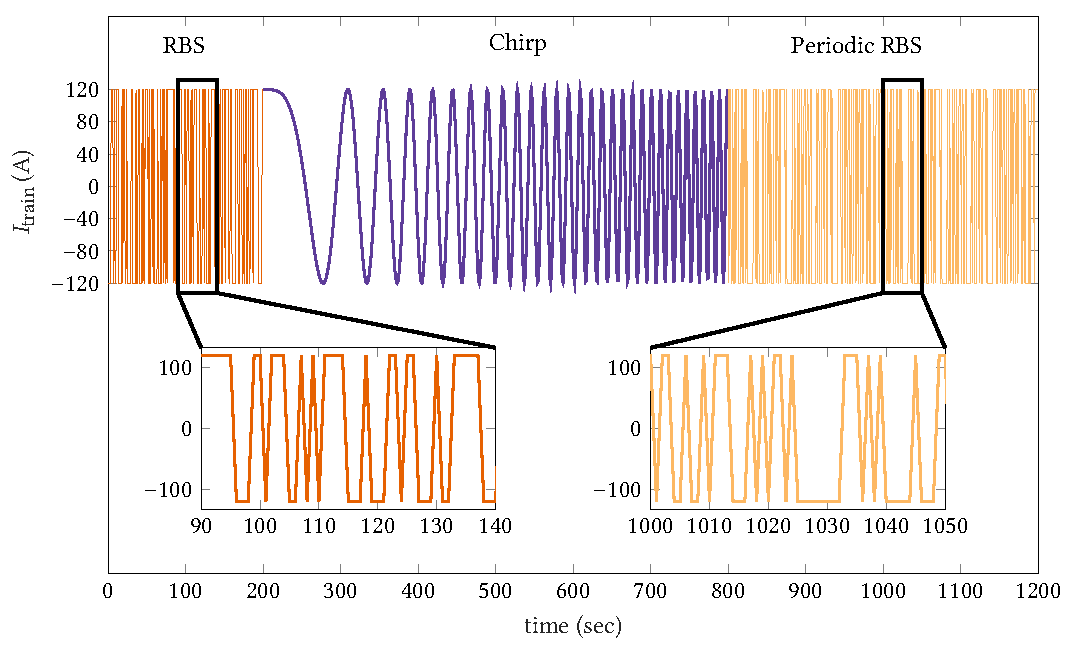
\includegraphics{sysid_train_input.pdf}
    \captionsetup{singlelinecheck=off}
    \caption[Input current profile used as the training set for system
    identification]{Input current profile used as the training set for system
    identification. The sequence consists of
    \begin{enumerate*}[label=\emph{\alph*})] \item a \glsfmtlong{rbs}, \item a
        chirp or swept cosine signal (0--\SI{100}{\milli\hertz}), and \item a periodic \glsfmtlong{rbs} \end{enumerate*} thereby
covering both low and high frequency spectra while incorporating the potential
to excite any periodic modes in the system to be identified.}
    \label{fig:sysidtrainingcurrent}
\end{figure}
Since not much prior  information is available about the poles  and zeros of the
electrolyte subsystem  in question, a wide  variety of special waveforms  with a
sampling interval of \SI{1}{\second} were used for the current perturbation used
in this system identification task. The specific input sequence consisted of
\begin{enumerate}
    \item \gls{rbs}\quad (0--\SI{199}{\second})
    \item `Chirp' \ie{} a swept cosine signal from 0--\SI{100}{\milli\hertz}\quad (200--\SI{799}{\second})
    \item Periodic \glsfmtlong{rbs} with a period of \SI{200}{\second} and 2 such periods\quad (800--\SI{1199}{\second})
\end{enumerate}
thereby helping to  obtain a wide-sense persistent excitation  signal. The swept
cosine  signal  is designed  to  excite  the low  frequency  (DC)  modes of  the
electrolyte subsystem and helps to capture the system's response to constant and
other systematically varying input profiles. The two \glspl{rbs} are intended to
target the poles and zeros of  the electrolyte subsystem that would typically be
excited  by  highly dynamic  input  profiles.  The  periodicity  in one  of  the
\glspl{rbs} was introduced  to draw out any hidden periodicity  or repeated real
poles  in the  system that  might  otherwise appear  to  be a  single pole.  The
presence  of both  low  and high  frequency frequency  spectra  in the  combined
training  set presents  a  high degree  of confidence  to  capture the  relevant
dynamics of the  electrolyte subsystem. The input current profile  used for this
system identification task is plotted in~\cref{fig:sysidtrainingcurrent}.

\subsection{Validation current profile}
For the  purposes of identification,  the \gls{p2d}  model is considered  as the
true system. First, the current profile from  the training set is applied to the
\gls{p2d} model. Its  simulation results, in particular,  the numerically solved
concentration values  at each spatially  discretised node  in each of  the three
regions per  time-step is then integrated  over the thickness of  the respective
regions  and multiplied  with their  respective porosities.  Thus the  number of
moles of \ch{Li^+}  per unit area in each of  the three regions $Q_{\text{e,}j}$
are obtained. Only  the quantities $Q_\text{e,n}$ and  $Q_\text{e,p}$ are chosen
as the outputs for system identification and a transfer function model is fitted
as per the evaluation procedure discussed in~\cref{subsubsec:actualsysid}.

As with  any classical  curve fitting  (numerical regression)  procedure, system
identification is also  prone to overfitting the training data.  In general, the
`best' transfer  function that identifies the  given system is the  lowest order
model that  can not  only minimize  the training error,  but also  minimizes the
error  on  a  previously  unseen  validation  dataset.  In  the  absence  of  an
independent validation dataset, the training error can be made arbitrarily small
by increasing  the number  of poles  and zeros of  the transfer  function models
without any  bounds. However, such a  model shall not have  truly identified the
dynamics of  the system  and shall  not generalise  well to  real-world datasets
outside  the training  realm. Hence,  having an  independent validation  current
profile for the task at hand is of paramount importance.

For the system identification task at  hand, the characteristic waveforms of the
validation profile were deliberately conjured to be differ vastly from that used
in training the model. The  validation profile consists of the following
sequence
\begin{enumerate}
    \item Periodic \gls{rgs} with 4 periods of \SI{200}{\second} each\quad (0--\SI{799}{\second})
    \item \gls{prbs} for emulating white noise, \ie{} with a flat power spectra
        across the frequency spectrum\quad (800--\SI{999}{\second})
    \item Multi-sine signal \ie{} a signal consisting of sinusoids at
        various fundamental frequencies added together\quad (1000--\SI{1199}{\second})
\end{enumerate}

Overall,  the validation  profile has  been designed  to cover  a wide  range of
frequencies  akin to  the  training  profile, but  differing  completely in  its
time-domain appearance.  The specific  validation current  profile used  in this
system identification is shown in~\cref{fig:sysidvalidationcurrent}.

\begin{figure}[!htb]
    \centering
    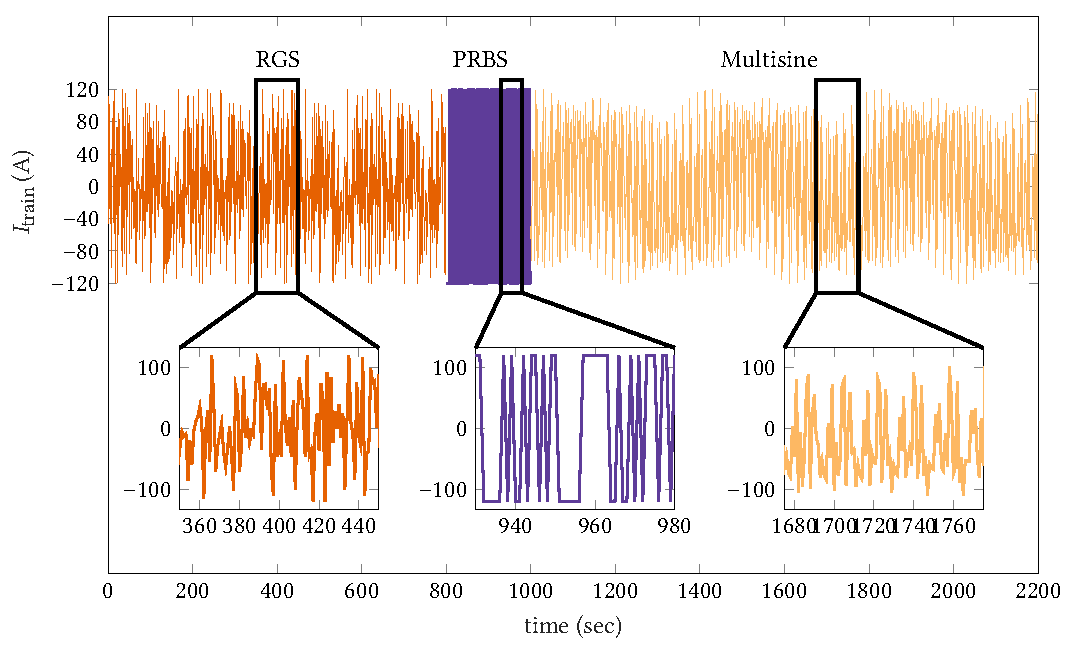
\includegraphics{sysid_validation_input.pdf}
    \captionsetup{singlelinecheck=off}
    \caption[Input current profile used as the validation set for system
    identification]{Input current profile used as the validation set for system
        identification. The sequence consists of
        \begin{enumerate*}[label=\emph{\alph*})]
            \item a \glsfmtlong{rgs},
            \item a \glsfmtlong{prbs}, and
            \item a multisine waveform
        \end{enumerate*}.
        The overall sequence  is intended to emulate the flat  power spectrum of
        white noise (with the \glsfmtshort{prbs}) and excite any poles and zeros
        within  3$\sigma$ spread  of the  \glsfmtshort{rgs} mean.  The multisine
        signal is  swept is composed  of sinusoids with  fundamental frequencies
        from \SI{100}{\milli\hertz}  up to the Nyquist  frequency. Its amplitude
        variation  across the  frequency spectrum  increases the  probability to
        capture the  system's modes that  were possibly missed by  the preceding
        two waveforms.
    }%
    \label{fig:sysidvalidationcurrent}
\end{figure}

\textsc{MATLAB} code  that can be used  to generate the training  and validation
input profiles is shown in~\cref{codesnippet:trainvalidsysidinput}.

\begin{listing}[!htbp]
\begin{minted}[mathescape,autogobble,bgcolor=mintedbg,escapeinside=||,texcomments=true]{matlab}
% Needs matlab's system identification toolbox
clear; close all; clc; format short g;
warning('off','Ident:dataprocess:idinput7'); % suppress sysid warnings
I_1C  = 60; % Amps
range = 2*[-I_1C I_1C]; % peak-peak swing is $\pm 2\text{C}=\SI{40}{\ampere}$
NumCh = 1; % no of channels (used by sysid toolbox for multichannel id)
Ts    = 1; % sampling interval

%% Random Binary Input Signal (RBS)
N  = 200; % samples per quantum of each waveform
u1 = idinput(N,'rbs',[],range); % 'idinput' from sysid toolbox
%% Chirp Signal (swept cosine)
t_chirp_start = 0;
t_chirp_end   = 3*N*Ts; %
t             = linspace(t_chirp_start,t_chirp_end,3*N);
f0            = 0;
f1            = 1e-1; % $f_1 = \SI{100}{\milli\hertz}$ is the max chirp frequency
u2            = max(range)*chirp(t,f0,t(end),f1)';
%% Periodic Random Binary Input Signal (Periodic RBS)
bin_seq_Period   = N; % seconds
bin_seq_Period_N = ceil(bin_seq_Period/Ts); % samples
bin_NumPeriod    = 2;
u3 = idinput([bin_seq_Period_N,NumCh,bin_NumPeriod],'rbs',[],range);
%% Random Guassian Signal (RGS)
rgs_Period         = N; % seconds
rgs_Period_samples = ceil(rgs_Period/Ts);
rgs_NumPeriod      = 4;
u4 = idinput([rgs_Period_samples,NumCh,rgs_NumPeriod],'rgs',[],range/2);
%% PseudoRandom Binary Signal (PRBS)
prbs_Period         = N; % seconds
prbs_Period_samples = ceil(prbs_Period/Ts);
u5                  = idinput(N,'prbs',[],range);
%% Multisine signal (sum of sines)
samples_per_Period = 2*N;
NumPeriod          = 3;
[u6,freq] = idinput([samples_per_Period 1 NumPeriod],'sine',[],range);

%% Split into training and validation data sets
I_load_train    = [u1;u2;u3];
I_load_validate = [u4;u5;u6];
\end{minted}
\caption{Generation of training and validation input current profiles in
\textsc{MATLAB}}
\label{codesnippet:trainvalidsysidinput}
\end{listing}

% Linearity and time-invariance

\section{Test for Linearity and Time Invariance}\label{sec:lticheck}
The      transfer     function      identification     techniques      mentioned
in~\cref{subsubsec:introblackboxsysid}   are  applicable  only   for   \gls{lti}
systems.  At the  first glance,  this seems  overly restrictive  for the  system
at  hand.  A lithium  ion  battery,  when  considered  as a  single  macroscopic
entity,  exhibits non-linear  characteristics,  particularly due  to the  strong
non-linearities in
\begin{enumerate*}[label=\emph{\alph*})]
    \item the Butler-Volmer reaction kinetics (see~\cref{eq:butlervolmer}), and
    \item the \glspl{ocp} of the two electrodes (see~\cref{eq:lcoUocpPos} and~\cref{eq:lcoUocpPos}).
\end{enumerate*}
However, since we are dealing with a much narrower scope \ie{} the systems under
consideration  are just  the two  sub-system entities  (one per  electrode) that
transform the  applied current at  a particular  time-step to the  overall moles
per  unit area  of  \ch{Li^+}  ions in  the  corresponding  electrode region  of
the  electrolyte at  that  same  instant. Therefore,  it  is  the linearity  and
time-invariance of these \emph{subsystems} that must be investigated.

\subsection{Time-invariance of the electrolyte time-evolution subsystems}\label{subsubsec:timeinvariance}
A  test  for time-invariance  is  prescribed  in  the  lecture notes  on  system
identification by  Plett~\cite{PlettECE5560_02}. The steps involved  therein are
reproduced here after  being suitably adapted to the notation  of the subsystems
at hand.
\begin{enumerate}
    \item Apply input $u_1(t) = I(t)$ to the system and measure the outputs $Q_{\text{e,n}_1}\!(t)$ and $Q_{\text{e,p}_1}\!(t)$.
    \item Apply a delayed version of the input by $\tau$ seconds \ie{} $u_2(t) = I(t-\tau)$ to the system and measure the outputs $Q_{\text{e,n}_2}\!(t)$ and $Q_{\text{e,n}_2}\!(t)$.
    \item If $Q_{\text{e,n}_2}\!(t)$ = $Q_{\text{e,n}_1}\!(t-\tau)$ and $Q_{\text{e,p}_2}\!(t)$ = $Q_{\text{e,p}_1}\!(t-\tau)$ for all possible delays $\tau$ as well as for choice of input signals $I(t)$, then the systems are time-invariant.
\end{enumerate}

For  the  systems   at  hand,  it  is  not  strictly   required  to  apply  this
prescriptive  test.  Unless a  fundamental  change  in the  underlying  reaction
phenomena/chemistry  occur that  alter the  performance over  time, systems  are
treated  as time-invariant.  Factors  that induce  time-dependent  shift in  the
behaviour of lithium ion batteries  are degradation phenomena such as thickening
of \gls{sei} layer  on the electrodes, dendrite growth or  mechanical fatigue in
electrodes  which in-turn  affect electrolytic  diffusion and  conductivity. Yet
another cause  of time-dependent  behavioural change is  the drift  in parameter
values. However, these  phenomena are typically one or mode  orders of magnitude
slower than  the \gls{p2d} dynamics\fxnote{citation needed}.  This separation of
time-scales  imply  that in  practice,  they  can  be decoupled  and  therefore,
separate  models can  be  identified  for the  faster  and  slower processes.  A
suitable model-blending approach  can then be considered to arrive  at cover all
processes across time-scales. Although the  concepts developed here for the fast
electrolyte dynamics can be suitably adapted to such slow phenomena, their study
falls outside  the scope of this  thesis and is  left as an exercise  for future
work.  Thus,  the overall  battery  system,  and  hence  by extension,  the  two
subsystems considered are deemed to  be time-invariant. However, in the interest
of  completeness, this  author  systematically applied  the aforementioned  test
procedure  with every  combination arising  from  the choice  of ten  time-delay
values and the following six current profiles ---
\begin{enumerate*}[label=\emph{\alph*})]
    \item constant current 1C discharge,
    \item constant current 3C discharge,
    \item constant current 1C charge,
    \item \gls{udds} input profile with peak amplitude of 3C,
    \item training profile used in system identification (see~\cref{fig:sysidtrainingcurrent}), and
    \item validation profile used in system identification (see~\cref{fig:sysidvalidationcurrent}).
\end{enumerate*}
Finally,  these tests  were  repeated for  a choice  of  five different  initial
\glspl{soc}   ---   \SI{90}{\percent},   \SI{70}{\percent},   \SI{50}{\percent},
\SI{30}{\percent}  and \SI{10}{\percent}\footnote{\label{fn:socstart}The  number
of  moles  of  \ch{Li^+} per  unit  area  in  the  electrolyte does  not  depend
on  the  electrode's \glsfmtshort{soc}.  However,  different  starting point  of
\glsfmtshort{soc}s were considered  to have a wide variety in  the length of the
recorded  data until  cut-offs  were hit.  \eg{}  starting at  \SI{90}{\percent}
\glsfmtshort{soc} could  mean that  for a  current spike  early in  the profile,
upper  cut-off voltage  shall be  hit  sooner leaving  a smaller  set of  logged
simulation data.}.

\begin{figure}[!htb]
    \centering
    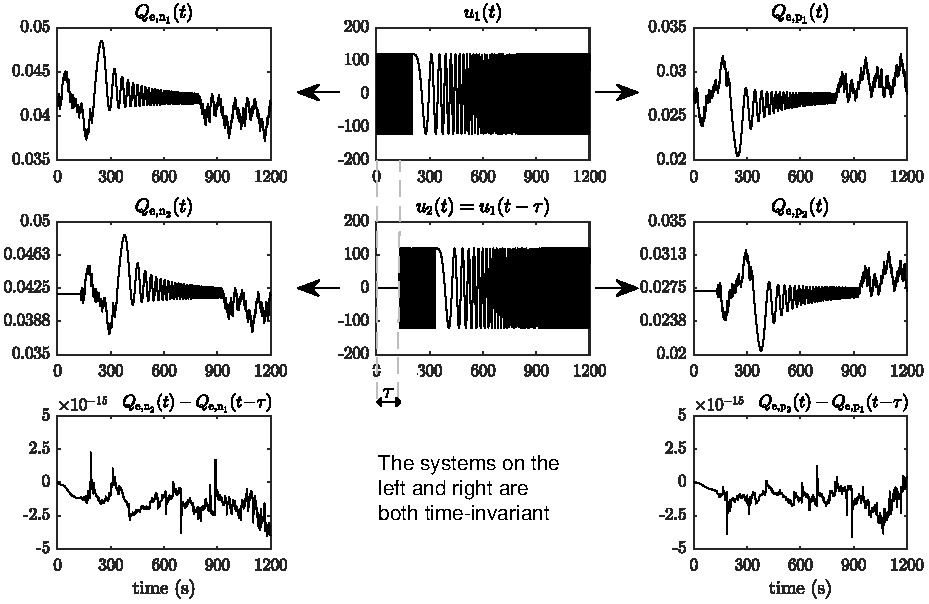
\includegraphics[width=\textwidth]{time_invariance.pdf}
    \caption[Demonstration of time-invariance of $Q_\text{e,n}(t)$ and
    $Q_\text{e,p}(t)$ subsystems]{Demonstration of time-invariance of the
        subsystems considered. The applied current profile $u_1(t)$ is the
        system identification training sequence
        from~\cref{fig:sysidtrainingcurrent} (top row of the central column).
        The top left plot shows the response $Q_{\text{e,n}_1}\!(t)$, while that
        on the top right shows $Q_{\text{e,p}_1}\!(t)$. The second row of the
        middle column shows the same input sequence delayed by $\tau =
        \SI{130}{\second}$. Application of this current profile $u_2(t) =
        u_1(t-\tau)$ results in the outputs $Q_{\text{e,n}_2}\!(t)$ and
        $Q_{\text{e,p}_2}\!(t)$ to its left and right respectively. Subtracting
        these from the correspondingly delayed versions of the original outputs
        result in zero residuals, thereby proving time-invariance of these
        subsystems. The jitter shown in the bottom row of plots is
        $\mathcal{O}(10^{-15})$ in magnitude and are due to the numerical
        roundoffs that occur when operating close to the noise floor of the
    machine's floating point units.}%
\label{fig:timeinvariance}
\end{figure}
% The outputs $Q_\text{e,n}$ and $Q_\text{e,p}$ are shown to the left and right of the applied input.

\Cref{fig:timeinvariance}  demonstrates the  time-invariance  of the  subsystems
considered  at an  initial \gls{soc}  of \SI{50}{\percent}  for a  time-delay of
\SI{130}{\second}  using  the  highly  dynamic  system  identification  training
sequence  that  was synthesised  by  this  thesis  author. The  applied  current
profile  $u_1(t)$  (top  row  of   the  central  column)  produces  the  outputs
$Q_{\text{e,n}_1}\!(t)$ and  $Q_{\text{e,p}_1}\!(t)$ shown  in the top  left and
top right  plots respectively. When the  delayed version of this  input sequence
${u_2(t) = u_1(t-\tau)}$  (middle row, middle column) is applied,  it results in
the outputs $Q_{\text{e,n}_2}\!(t)$ and  $Q_{\text{e,p}_2}\!(t)$ to its left and
right respectively. Following the steps of the test procedure, subtracting these
outputs from the correspondingly delayed versions of their original counterparts
result in  zero residuals, thereby  proving time-invariance of  these subsystems
under these representative test conditions. The residual sequences in the bottom
row of plots are of $\mathcal{O}(10^{-15})$ and arise due to numerical roundoffs
that occur  when operating close  to the noise  floor of the  machine's floating
point units.

Similar to  the case demonstrated  here, all  tests for time-invariance  for all
permutations of  the chosen operating  conditions passed successfully  \ie{} the
delayed  version of  the original  output  signals accurately  matched with  the
responses  to  the corresponding  delayed  input  (down to  machine  precision),
thereby confirming the time-variance of  the subsystems considered in the system
identification problem, which enables us to proceed further.


\subsubsection*{Linearity   analysis    of   the    time-evolution   electrolyte
subsystems}\label{subsubsec:linearityanalysis}

In the analyses of linearity of systems, it is a recommended practice to de-bias
the output and input quantities about their mean operating conditions. The input
signal in  this case,  is the  applied load  current $I(t)$,  which can  be both
positive (during  discharge) and negative  (during charge). Although  in typical
drive-cycles there  is a net  discharge, the value  of the mean  applied current
differs across  drivecycles. Furthermore, drivecycles are  merely representative
profiles and therefore, in real-world operation, the cell needs to be treated as
being equally  probable for being  subjected charged and discharged.  Hence, the
mean  of the  input signal  is taken  as zero,  which eliminates  any de-biasing
requirements.

For  the output  signals  though, bias  values can  be  clearly identified.  The
overall number of moles of \ch{Li^+} per unit area in any region within the cell
cannot be physically negative. Even though  under high C-rates, ion depletion at
localised  spatial  locations (such  as  the  current collectors)  is  certainly
possible, the entire thickness of any region cannot become devoid of ions at any
point in time  since the cell shall  instantaneously cease to work.  Thus, for a
typical well-designed  cell operating within the  manufacturer prescribed C-rate
limits, the output  signals under consideration operate in a  small window about
their initial values. In the author's  simulations, even at $\pm$5C, the overall
number of moles  of \ch{Li^+} in any  cell region exhibited a  maximum change of
less than \SI{15}{\percent}  from its initial value. Thus,  the de-biased output
variables  for  system  identification, $\widetilde{Q}_{\text{e,}j}(t)$  can  be
obtained  by subtracting  their  respective  initial values  $Q_{\text{e,}j}(0)$
(see~\cref{eq:Qeninit} and~\cref{eq:Qepinit}) from $Q_{\text{e,}j}(t)$.
\begin{align}
    \widetilde{Q}_\text{e,n}(t) & = {Q}_\text{e,n}(t) - {Q}_\text{e,n}(0) \\
    \widetilde{Q}_\text{e,p}(t) & = {Q}_\text{e,p}(t) - {Q}_\text{e,p}(0)
\end{align}
which   implies   that   the   transfer  functions   to   be   identified   have
to   be   modified    to   be   $\frac{\widetilde{Q}_\text{e,n}(s)}{I(s)}$   and
$\frac{\widetilde{Q}_\text{e,p}(s)}{I(s)}$  respectively. This  does not  affect
the time-invariance proved  in~\cref{subsubsec:timeinvariance} since the initial
values $Q_{\text{e,}j}(0)$ are merely constants and hence not time-dependent.

Similar     to      the     test      for     time      invariance     described
in~\cref{subsubsec:timeinvariance}, a  test for linearity is  also prescribed in
the lecture notes on  system identification by Plett~\cite{PlettECE5560_02}. The
steps involved therein  are reproduced here after being suitably  adapted to the
notation of the subsystems at hand. This is essentially a recipe for testing the
superposition principle.
\begin{enumerate}
    \item Apply input profile $I_1(t)$ to the system and obtain outputs $\widetilde{Q}_{\text{e,n}_1}\!(t)$ and $\widetilde{Q}_{\text{e,p}_1}\!(t)$.
    \item Apply a different profile $I_2(t)$ to the system and obtain outputs $\widetilde{Q}_{\text{e,n}_2}\!(t)$ and $\widetilde{Q}_{\text{e,n}_2}\!(t)$.
    \item Now apply an input profile $I_3(t) = \alpha I_1(t) + \beta I_2(t)$ and obtain a corresponding set of outputs $\widetilde{Q}_{\text{e,n}_3}\!(t)$ and $\widetilde{Q}_{\text{e,n}_3}\!(t)$.
    \item If $\widetilde{Q}_{\text{e,n}_3}\!(t)$ = $\alpha\, \widetilde{Q}_{\text{e,n}_1}\!(t) + \beta \, \widetilde{Q}_{\text{e,n}_2}\!(t)$ and $\widetilde{Q}_{\text{e,p}_3}\!(t)$ = $\alpha\, \widetilde{Q}_{\text{e,p}_1}\!(t) + \beta \, \widetilde{Q}_{\text{e,p}_2}\!(t)$ for all possible $\{\alpha,\beta\}$ as well as for choice of input signals $\{I_1(t),I_2(t)\}$, then the systems are linear.
\end{enumerate}

Similar  to   the  time-invariance  test,   the  same  set  of   five  different
initial  \glspl{soc}\ref{fn:socstart} ---  \SI{90}{\percent}, \SI{70}{\percent},
\SI{50}{\percent},  \SI{30}{\percent} and  \SI{10}{\percent},  was retained  for
these linearity tests.  For each test run, a pseudo-random  number generator was
used to  select the values  of $\{\alpha,\beta\}$ from  the set of  real numbers
$\mathbb{R}$ (not restricted to the set  of integers $\mathbb{Z}$) in the closed
interval spanning  $[-1.25,1.25]$. Negative values  are acceptable for  both the
scaling coefficients since the resulting  composite input $I_3(t)$ can be either
positive or  negative. The composite  signal $I_3(t)$  was obtained by  taking a
random combination of any two of the following current profiles ---
\begin{enumerate*}[label=\emph{\alph*})]
    \item constant current 1C discharge,
    \item constant current discharge at C/5,
    \item constant current 1C charge,
    \item constant current charge at C/5,
    \item training profile used in system identification (see~\cref{fig:sysidtrainingcurrent}), and
    \item validation profile used in system identification (see~\cref{fig:sysidvalidationcurrent}).
\end{enumerate*}

The  scaling  factors  $\alpha$  and   $\beta$  were  restricted  to  the  range
$[-1.25,1.25]$ in consideration of limiting the peak applied current to within a
\pm 5C  window ---  the operating  condition for most  \glspl{bev}, so  that the
isothermal assumption for the model shall remain valid. This peak current corner
case occurs when the pseudo-random generator chooses both scaling factors at the
selected range's limits for the 1C constant current discharge or charging cases.
The limited  range of the  scaling factors are also  motivated by the  fact that
most real-world systems remain linear only within a certain operating window. In
particular, care  must be taken to  ensure that the cell's  \gls{soc} during the
linearity test  remains within  its physical limits  for any  initial \gls{soc}.
Furthermore, localised  saturation or depletion  of ions for  extended durations
must be avoided. Hence  it can be concluded that, with the  chosen range for the
scaling  factors,  if  the  two subsystems  under  consideration  remain  linear
everywhere below  a peak  current of  \pm 5C  in the  isothermal case,  then the
linearity  tests are  considered as  passed.  Future extensions  to undertake  a
temperature-dependent  system  identification  exercise can  potentially  use  a
first-order Taylor  expansion about this  operating window. The  discussion thus
far has fully established all the conditions for conducting the for linearity.

\begin{figure}[!htb]
    \centering
    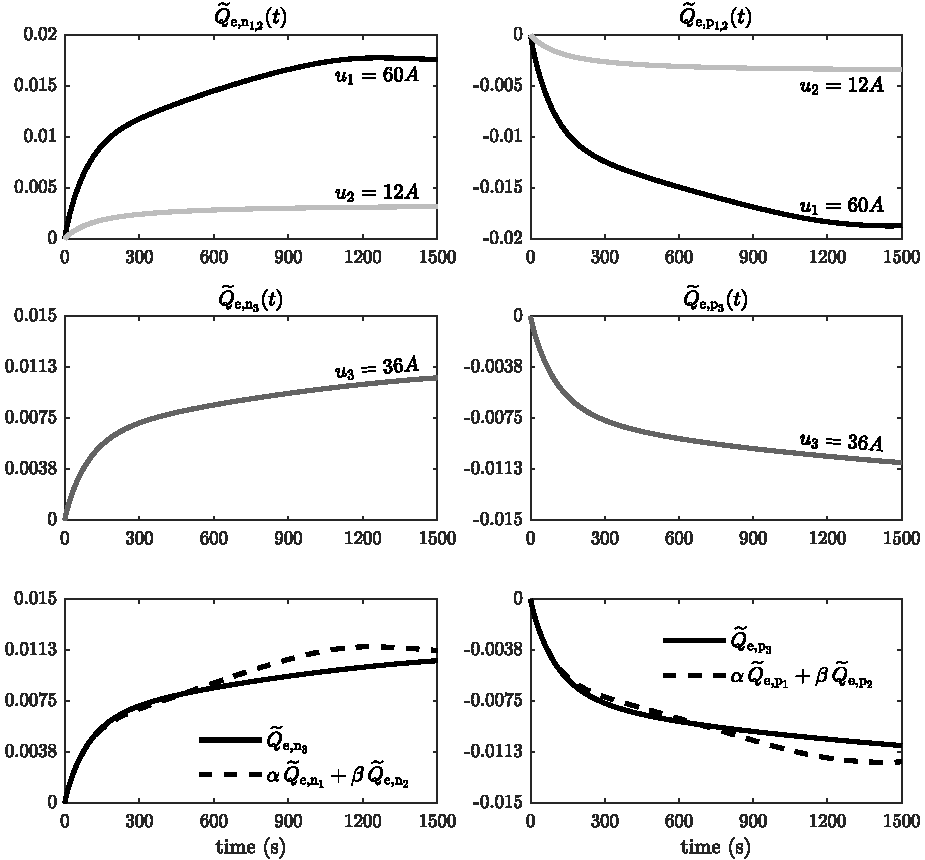
\includegraphics[width=\textwidth]{linearity_proof}
    \caption[Illustration of linearity test for the
    \protect{$\widetilde{Q}_{\text{e,n}}$} and
    \protect{$\widetilde{Q}_{\text{e,p}}$} subsystems]{Illustration of one
        instance of linearity tests for the subsystems under consideration. For
        this visualisation, constant current inputs are used throughout. The top
        row of plots shows $\widetilde{Q}_{\text{e,n}}$ and
        $\widetilde{Q}_{\text{e,p}}$ for two input currents $I_1(t) =
        \SI{60}{\ampere}$ and $I_2(t) = \SI{12}{\ampere}$ \ie{} discharge with
        1C and C/5 currents respectively. The second row of plots shows
        $\widetilde{Q}_{\text{e,n}_3}$ and $\widetilde{Q}_{\text{e,p}_3}$  for
        $I_3 = \SI{36}{\ampere}$, where $I_3 = \alpha I_1 + \beta I_2$ with
        $(\alpha,\beta) = (1,-2)$. The last row of plots overlays these
        quantities with the manually computed linear combination of their two
        preceding responses. Had these sequences overlapped exactly, the systems
        would have been exactly linear. Despite exhibiting deviations over the
        considered horizon, the transient responses in both electrode regions do
        follow the superposition principle. Even past the transient, maximum
        error in both cases is an order of magnitude lower than the individual
        outputs. Hence, the two systems are deemed to be \emph{approximately}
        linear.
    }%
    \label{fig:linearity}
\end{figure}

\Cref{fig:linearity}  illustrates  one  instance  of a  linearity  test  wherein
constant  currents  and  integer  scaling  factors are  used  for  the  sake  of
illustration.  The  plots   in  the  left  column  deal   with  the  electrolyte
time-evolution  subsystem  in  the  negative electrode  region.  Similarly.  the
plots  in  the  right  column  deal with  the  corresponding  subsystem  in  the
positive electrode region.  A discharge current of 1C  \ie{} \SI{60}{\ampere} is
first  applied  and  the  corresponding  outputs  $\widetilde{Q}_{\text{e,n}_1}$
and   $\widetilde{Q}_{\text{e,p}_1}$  are   obtained.   Secondly,  a   discharge
current   of   C/5   \ie{}   is    applied   and   the   corresponding   outputs
$\widetilde{Q}_{\text{e,n}_2}$ and  $\widetilde{Q}_{\text{e,p}_2}$ are obtained.
These set of responses are plotted  in the top row of~\cref{fig:linearity}. Now,
a  third  value  of  input  current $I_3$,  computed  as  a  linear  combination
of  the  previous  input  currents  \ie{}  $I_3 =  \alpha  I_1  +  \beta  I_2  $
is  applied.  For  illustrative  purposes, the  integer  set  $(\alpha,\beta)  =
(1,-2)$  was  chosen  for  the   scaling  coefficients,  which  implies  $I_3  =
\SI{12}{\ampere}$. The corresponding  outputs $\widetilde{Q}_{\text{e,n}_3}$ and
$\widetilde{Q}_{\text{e,p}_3}$ are  plotted in the  middle row. As per  the test
for linearity,  if these signals are  equal to the signal  generated by manually
computing the linear  combination of the preceding two outputs,  then the system
is linear.

The   plots   in  the   third   row   show  $\widetilde{Q}_{\text{e,n}_3}$   and
$\widetilde{Q}_{\text{e,p}_3}$ overlaid with their respective linear combination
signals. In  the case  of the  subsystem in the  negative electrode  region, the
transient performance matches  precisely until \approx\SI{450}{\second}, whereas
that in the positive electrode region exhibits a good matching for approximately
the  first  \SI{250}{\second}.  However,  for the  horizon  considered  the  two
overlaid plots do not overlap exactly.  Hence, the systems are not truly linear.
However, the exhibited  behaviour is quite close to linearity,  with the maximum
absolute  error  in each  region,  even  outside  the initial  transient,  being
$\mathcal{O}(10^{-4})$  --- an  order  of magnitude  lower  than its  individual
components.  This behaviour  was exhibited  for all  test instances  considered.
Considering  that for  dynamic  simulation runs,  the  transient performance  is
paramount  to  the good  performance  of  the  model,  in conjunction  with  the
aforementioned  low error  metric,  these  subsystems can  be  considered to  be
\emph{approximately} linear.


% Discussion of identification choices here

\subsection{Identification Methodology and Governing Equations}\label{subsubsec:actualsysid}
\subsection{Performance of Final Model}
\section{Embedding into SPM and final results for composite system}

% Assumed transfer function model. Test results within the model itself
% Test results for electrolyte ce (subsection)
% test results for full system (final section)

% mention in introduction where code snippets are given

 % New Electrolye Model

\cleardoublepage

\begin{footnotesize} % tiny(5) < scriptsize(7) < footnotesize(8) < small (9)
    \renewcommand{\bibname}{References} % changes the header; default: Bibliography
    % add bib to toc
    \cleardoublepage
    \phantomsection
    \addcontentsline{toc}{chapter}{\bibname}
    \printbibliography
\end{footnotesize}

\cleardoublepage

\begin{appendices} % Using appendices environment for more functionality
    \crefalias{chapter}{appchap}
    % -*- root: ../main.tex -*-
%!TEX root = ../main.tex
% vim: nospell

% ******************************* Thesis Appendix A ****************************
\chapter{Full Listing of Program Codes}

% dummy cts time \label{sc:ctstimespm}
\matlabcodelisting[\textsc{MATLAB} code for simulation of continuous time \glsfmtshort{spm}]{Appendices/matlab_codes/cts_time_spm_simulation.m}{sc:ctstimespm}

% dummy disc time\label{sc:disctimespm}
\clearpage
\matlabcodelisting[\textsc{MATLAB} code for simulation of discrete time \glsfmtshort{spm}]{Appendices/matlab_codes/disc_time_spm_simulation.m}{sc:disctimespm}

% graphviz doc in appendix, toolbox, directory listing etc.

    % -*- root: ../main.tex -*-
%!TEX root = ../main.tex
% vim: nospell

% ******************************* Thesis Appendix A ****************************
\chapter{Permissions Summary}\label{ch:permissions}

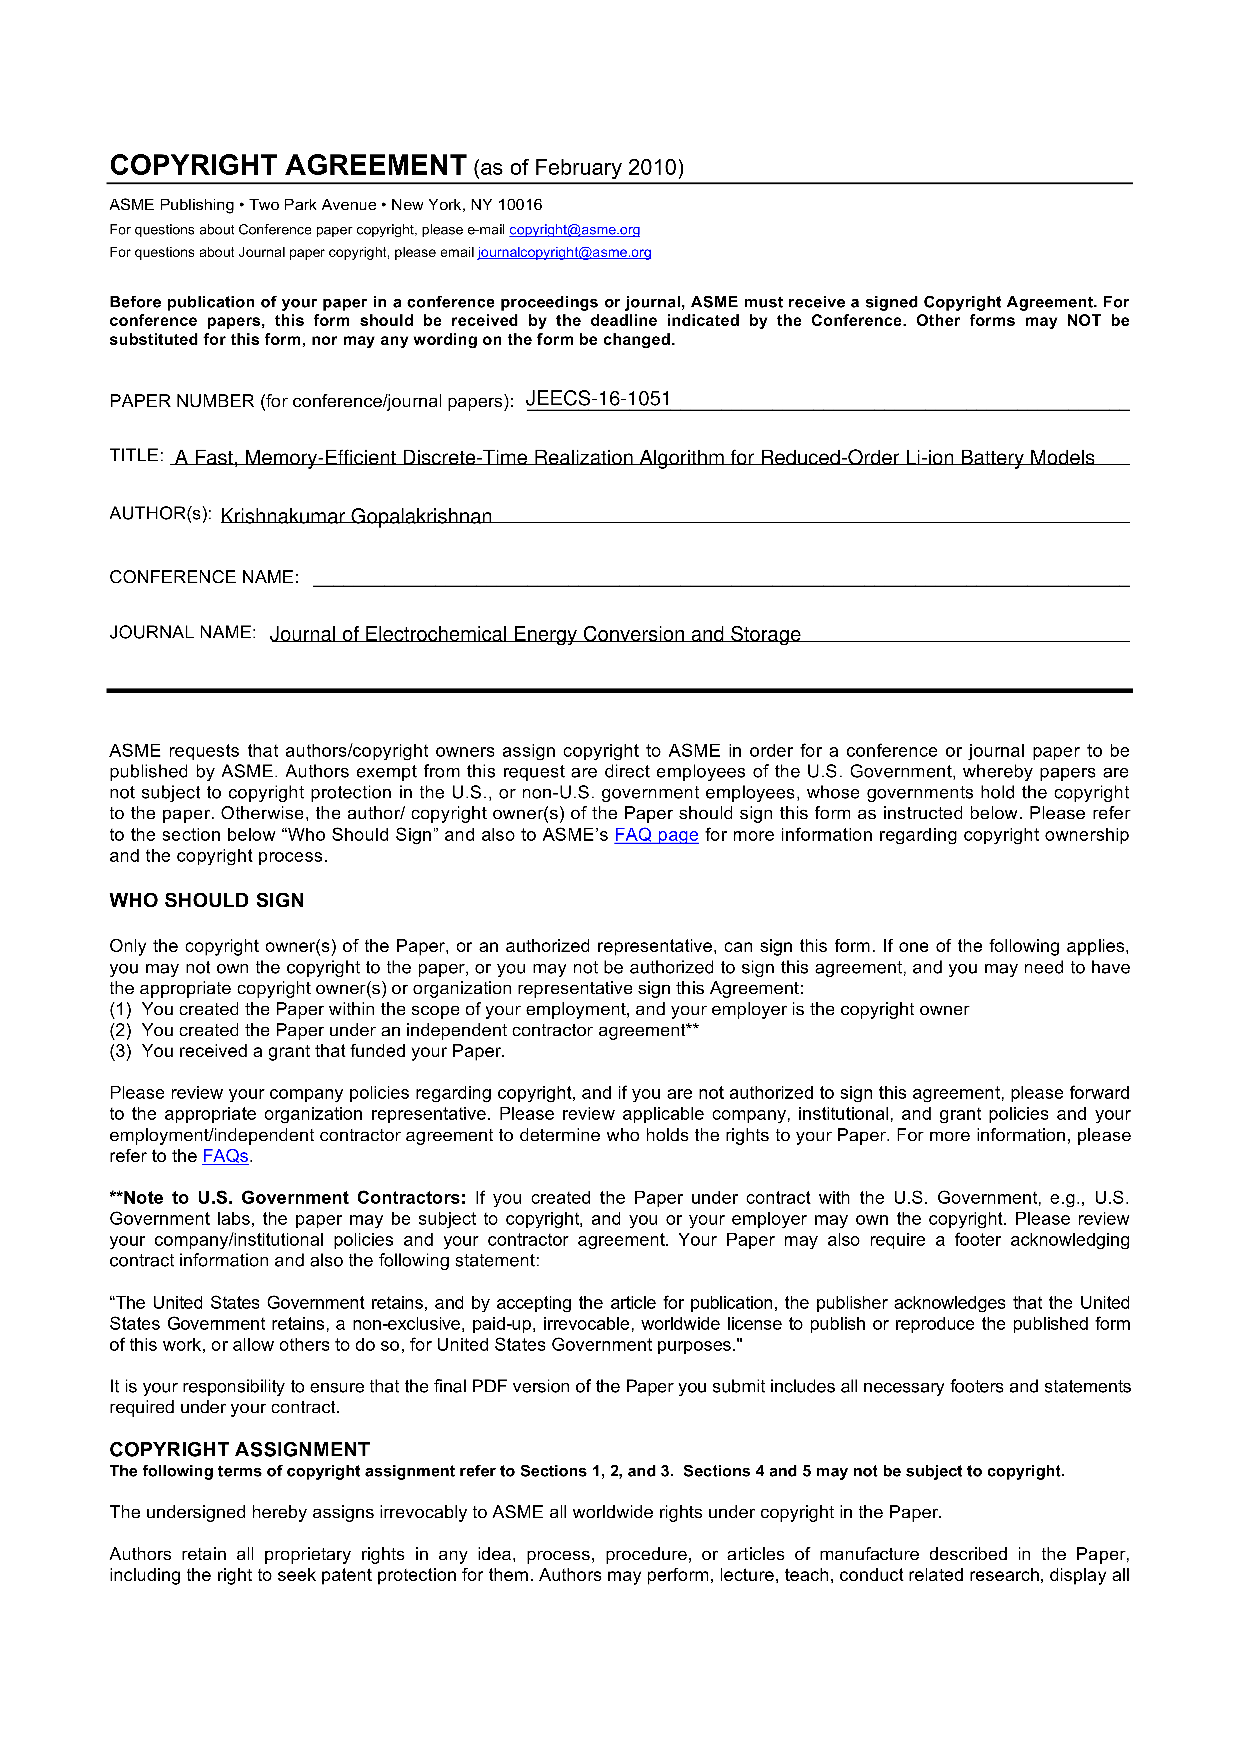
\includepdf[pages=-]{Appendices/asme_copyright.pdf}




\end{appendices}

% \backmatter


\batchmode
\end{document}
